% =============================================================================
% RAPPORT DE STAGE DE FIN D'ANNEE
% Plateforme Maroc Affiliate Network
% Auteur : Aymane
% Encadrant : Khalid Echchahid
% =============================================================================

\documentclass[12pt,a4paper,openany]{report}

% ---------------------------------------------------------------------------
% Encodage et langue
% ---------------------------------------------------------------------------
\usepackage[utf8]{inputenc}
\usepackage[T1]{fontenc}
\usepackage[french]{babel}

% ---------------------------------------------------------------------------
% Mise en page
% ---------------------------------------------------------------------------
\usepackage[
  a4paper,
  top=2.5cm, bottom=2.5cm,
  left=3cm, right=2.5cm
]{geometry}
\usepackage{setspace}
\onehalfspacing
\raggedbottom

% Profondeur de numérotation et de table des matières
\setcounter{secnumdepth}{2}
\setcounter{tocdepth}{2}

% Éviter lignes orphelines/veuves
\widowpenalty=10000
\clubpenalty=10000

% Éviter les titres seuls en bas de page
\usepackage{needspace}
\makeatletter
\renewcommand\section{\@startsection{section}{1}{\z@}%
  {-3.5ex \@plus -1ex \@minus -.2ex}%
  {2.3ex \@plus.2ex}%
  {\needspace{10\baselineskip}\normalfont\Large\bfseries\color{primary}}}
\renewcommand\subsection{\@startsection{subsection}{2}{\z@}%
  {-3.25ex\@plus -1ex \@minus -.2ex}%
  {1.5ex \@plus .2ex}%
  {\needspace{8\baselineskip}\normalfont\large\bfseries\color{primary!80!black}}}
\makeatother

% ---------------------------------------------------------------------------
% Typographie
% ---------------------------------------------------------------------------
\usepackage{lmodern}
\usepackage{microtype}

% ---------------------------------------------------------------------------
% Mathématiques
% ---------------------------------------------------------------------------
\usepackage{amsmath}
\usepackage{amssymb}

% ---------------------------------------------------------------------------
% Tableaux
% ---------------------------------------------------------------------------
\usepackage{booktabs}
\usepackage{array}
\usepackage{tabularx}
\usepackage{longtable}
\usepackage{multirow}
\usepackage[table]{xcolor}

% ---------------------------------------------------------------------------
% Figures et graphiques
% ---------------------------------------------------------------------------
\usepackage{graphicx}
\usepackage{float}
\usepackage{caption}
\usepackage{subcaption}
\usepackage{tikz}
\usetikzlibrary{shapes.geometric, arrows.meta, positioning, fit, calc, shapes, backgrounds}

% Chemin des images
\graphicspath{{figures/}{PFAimages/}}

% ---------------------------------------------------------------------------
% Code source
% ---------------------------------------------------------------------------
\usepackage{listings}
\usepackage{inconsolata}

% ---------------------------------------------------------------------------
% Boîtes colorées
% ---------------------------------------------------------------------------
\usepackage{tcolorbox}
\tcbuselibrary{skins, breakable}

% ---------------------------------------------------------------------------
% En-têtes et pieds de page
% ---------------------------------------------------------------------------
\usepackage{fancyhdr}
\pagestyle{fancy}
\fancyhf{}
\fancyhead[L]{\small\textit{\leftmark}}
\fancyhead[R]{\small\textit{Maroc Affiliate Network}}
\fancyfoot[C]{\thepage}
\renewcommand{\headrulewidth}{0.4pt}
\renewcommand{\footrulewidth}{0.4pt}
\setlength{\headheight}{14pt}

% Appliquer le même style aux pages de début de chapitre
\fancypagestyle{plain}{
  \fancyhf{}
  \fancyhead[L]{\small\textit{\leftmark}}
  \fancyhead[R]{\small\textit{Maroc Affiliate Network}}
  \fancyfoot[C]{\thepage}
  \renewcommand{\headrulewidth}{0.4pt}
  \renewcommand{\footrulewidth}{0.4pt}
}

% ---------------------------------------------------------------------------
% Divers
% ---------------------------------------------------------------------------
\usepackage{enumitem}
\usepackage{titlesec}
\usepackage{tocloft}
% Compacter légèrement la table des matières
\setlength{\cftbeforechapskip}{2pt}
\setlength{\cftbeforesecskip}{0.6pt}
\setlength{\cftbeforesubsecskip}{0.4pt}
\usepackage{pdfpages}

% ---------------------------------------------------------------------------
% Couleurs personnalisées
% ---------------------------------------------------------------------------
\definecolor{primary}{HTML}{1E40AF}
\definecolor{secondary}{HTML}{6B7280}
\definecolor{accent}{HTML}{059669}
\definecolor{codebg}{HTML}{F8FAFC}
\definecolor{codeframe}{HTML}{E2E8F0}
\definecolor{headerblue}{RGB}{31, 78, 121}
\definecolor{rowgray}{RGB}{242, 242, 242}

% ---------------------------------------------------------------------------
% Configuration des listings
% ---------------------------------------------------------------------------
\lstdefinestyle{typescript}{
  backgroundcolor=\color{codebg},
  basicstyle=\ttfamily\footnotesize,
  breaklines=true,
  captionpos=b,
  commentstyle=\color{secondary}\itshape,
  keywordstyle=\color{primary}\bfseries,
  stringstyle=\color{accent},
  frame=single,
  rulecolor=\color{codeframe},
  framerule=0.5pt,
  numbers=left,
  numberstyle=\tiny\color{secondary},
  tabsize=2,
  showstringspaces=false,
  xleftmargin=1.5em,
  morekeywords={interface, export, async, await, function, const, type, import, from, Promise, let, enum, model}
}
\lstset{style=typescript}

% ---------------------------------------------------------------------------
% Configuration des titres
% ---------------------------------------------------------------------------
\titleformat{\chapter}[hang]
  {\normalfont\LARGE\bfseries\color{primary}}
  {\chaptertitlename\ \thechapter\;--\;}{0pt}{}
\titlespacing*{\chapter}{0pt}{20pt}{15pt}

% ---------------------------------------------------------------------------
% Hyperliens (en dernier)
% ---------------------------------------------------------------------------
\usepackage{hyperref}
\hypersetup{
  colorlinks=true,
  linkcolor=primary,
  urlcolor=primary,
  citecolor=primary,
  pdftitle={Rapport de Stage - Plateforme Maroc Affiliate Network},
  pdfauthor={CHELLAK Aymane},
  breaklinks=true,
}

% Permettre les coupures dans les URLs et le code
\tolerance=1000
\emergencystretch=3em
\sloppy

% ---------------------------------------------------------------------------
% Commandes utilitaires
% ---------------------------------------------------------------------------
\newcommand{\ms}{\,ms}
\newcommand{\code}[1]{\texttt{#1}}

% =============================================================================
% DÉBUT DU DOCUMENT
% =============================================================================
\begin{document}

% =============================================================================
% PAGE DE GARDE
% =============================================================================
\begin{titlepage}
\centering
\vspace*{0.2cm}

\begin{minipage}{0.45\textwidth}
\centering
\includegraphics[width=4.0cm]{figures/fstmlogo.png}
\end{minipage}
\hfill
\begin{minipage}{0.45\textwidth}
\centering
\includegraphics[width=2.8cm]{figures/marocaffiliatelogo.png}
\end{minipage}

\vspace{0.6cm}

\rule{\linewidth}{0.8pt}
\vspace{0.2cm}

{\Large\bfseries\color{primary} Rapport de Stage de Fin d'Année}\\[0.3em]
{\large Cycle Ingénieur -- Data Science et Informatique}

\vspace{0.4cm}
\rule{\linewidth}{0.8pt}

\vspace{0.7cm}

{\Huge\bfseries IA Pratique pour une Plateforme\\[0.25em]
E-Commerce d'Affiliation}

\vspace{0.5cm}

{\large Recommandation de Produits, Intelligence d'Approvisionnement\\
et Analytics Métier.}

\vspace{0.8cm}

\begin{tabular}{@{}ll}
\textbf{Réalisé par :}           & CHELLAK Aymane \\[0.2em]
\textbf{Encadrant académique :}  & MOUSSAID Ahmed \\[0.2em]
\textbf{Encadrant entreprise :}  & ECHCHAHID Khalid \\[0.2em]
\textbf{Entreprise :}            & Maroc Affiliate -- \url{https://marocaffiliate.com} \\[0.2em]
\textbf{Période :}               & 06/04/2026 -- 06/06/2026 \\[0.2em]
\textbf{Année universitaire :}   & 2025--2026
\end{tabular}

\vfill

\rule{\linewidth}{0.4pt}
\vspace{0.3cm}

{\normalsize Soutenu le \textbf{18 juin 2026} devant le jury composé de :}

\vspace{0.3cm}

\begin{tabular}{ll}
\textbf{MOUSSAID Ahmed} & Faculté des Sciences et Techniques de Mohammedia \\[0.2em]
\textbf{BEN-LOHGHFYRY Anouar} & Faculté des Sciences et Techniques de Mohammedia \\
\end{tabular}

\vspace{0.4cm}
\rule{\linewidth}{0.8pt}
\vspace{0.2cm}

{\small Faculté des Sciences et Techniques de Mohammedia -- Département de Mathématiques}
\end{titlepage}

% =============================================================================
% REMERCIEMENTS
% =============================================================================
\chapter*{Remerciements}
\addcontentsline{toc}{chapter}{Remerciements}

Je tiens à exprimer ma sincère gratitude à toutes les personnes qui ont contribué à la réussite de ce stage.

Mes remerciements s'adressent en premier lieu à mon encadrant académique, \textbf{M. MOUSSAID Ahmed}, pour son suivi rigoureux, ses orientations méthodologiques et sa disponibilité tout au long de ce projet. Ses conseils m'ont permis de structurer mon travail et de maintenir un cap scientifique solide.

Je remercie chaleureusement mon encadrant en entreprise, \textbf{M. ECHCHAHID Khalid}, pour sa confiance, son exigence technique et son accompagnement quotidien. Sa vision produit et ses retours concrets m'ont permis de progresser significativement sur le plan professionnel.

Je remercie également l'équipe de \textbf{Maroc Affiliate Network} pour l'environnement de travail stimulant, la qualité des échanges techniques et la possibilité d'intervenir sur des problématiques réelles de production.

Enfin, je remercie mes enseignants de la Faculté des Sciences et Techniques de Mohammedia pour la formation solide qui m'a permis d'aborder ce stage avec les compétences nécessaires, ainsi que ma famille pour son soutien constant.

\newpage

% =============================================================================
% RÉSUMÉ
% =============================================================================
\chapter*{Résumé}
\addcontentsline{toc}{chapter}{Résumé}

Ce rapport présente le travail réalisé durant mon stage de fin d'études au sein de l'entreprise Maroc Affiliate Network. Le projet consiste en la conception et le développement d'une plateforme e-commerce multi-rôles d'affiliation destinée au marché marocain.

La plateforme permet à des vendeurs indépendants (affiliés) de commercialiser des produits via un réseau structuré, en gérant l'ensemble de la chaîne de valeur : catalogue, stock multi-entrepôts, commandes, livraison et facturation.

Mon stage s'est articulé autour de trois missions principales :

\begin{enumerate}
  \item \textbf{Module Analytics Dashboard} -- Conception et développement d'un système complet de tableaux de bord analytiques pour les administrateurs, comprenant 8 sous-tableaux couvrant les commandes, la livraison, les produits, les vendeurs, les clients et les entrepôts.

  \item \textbf{Système de Recommandation Intelligent} -- Développement d'un microservice autonome de recommandation de produits utilisant un algorithme à ensemble pondéré avec adaptation dynamique des poids selon le profil vendeur.

  \item \textbf{Module d'Enrichissement de Stock} -- Implémentation d'un système d'approvisionnement avec deux modes d'entrée (scanner QR et sélection manuelle), intégré au pipeline de transfert inter-entrepôts.
\end{enumerate}

\textbf{Technologies principales :} Next.js 15, TypeScript, PostgreSQL, Prisma, FastAPI, Redis, Docker.

\textbf{Mots-clés :} E-commerce, affiliation, multi-rôles, analytics, recommandation, stock, Next.js, microservices.

\newpage

% =============================================================================
% ABSTRACT
% =============================================================================
\chapter*{Abstract}
\addcontentsline{toc}{chapter}{Abstract}

This report presents the work carried out during my end-of-study internship at Maroc Affiliate Network. The project involves the design and development of a multi-role e-commerce affiliation platform for the Moroccan market.

The platform enables independent sellers (affiliates) to market products through a structured network, managing the entire value chain: catalog, multi-warehouse stock, orders, delivery, and billing.

My internship was organized around three main missions:

\begin{enumerate}
  \item \textbf{Analytics Dashboard Module} -- Design and development of a comprehensive analytics dashboard system for administrators, featuring 8 sub-dashboards covering orders, delivery, products, sellers, customers, and warehouses.

  \item \textbf{Intelligent Recommendation System} -- Development of a standalone product recommendation microservice using a weighted ensemble algorithm with dynamic weight adaptation based on seller profiles.

  \item \textbf{Stock Enrichment Module} -- Implementation of a procurement system with two input modes (QR scanner and manual selection), integrated with the inter-warehouse transfer pipeline.
\end{enumerate}

\textbf{Main technologies:} Next.js 15, TypeScript, PostgreSQL, Prisma, FastAPI, Redis, Docker.

\textbf{Keywords:} E-commerce, affiliation, multi-role, analytics, recommendation, stock, Next.js, microservices.

\newpage

% =============================================================================
% TABLE DES MATIÈRES
% =============================================================================
\tableofcontents

\newpage

% =============================================================================
% LISTE DES FIGURES
% =============================================================================
\listoffigures
\addcontentsline{toc}{chapter}{Liste des figures}

\newpage

% =============================================================================
% GLOSSAIRE
% =============================================================================
\chapter*{Glossaire}
\addcontentsline{toc}{chapter}{Glossaire}
\markboth{Glossaire}{Glossaire}

\begin{longtable}{lp{11cm}}
\toprule
\textbf{Acronyme} & \textbf{Définition} \\
\midrule
\endhead
API & Application Programming Interface -- Interface de programmation \\
ASGI & Asynchronous Server Gateway Interface -- Protocole serveur Python asynchrone \\
CDN & Content Delivery Network -- Réseau de distribution de contenu \\
CTE & Common Table Expression -- Expression de table commune en SQL \\
CRUD & Create, Read, Update, Delete -- Opérations de base sur les données \\
ERD & Entity-Relationship Diagram -- Diagramme entité-relation \\
KPI & Key Performance Indicator -- Indicateur clé de performance \\
LRU & Least Recently Used -- Politique d'éviction de cache \\
LTV & Lifetime Value -- Valeur client sur la durée \\
ML & Machine Learning -- Apprentissage automatique \\
ORM & Object-Relational Mapping -- Mapping objet-relationnel \\
POS & Point of Sale -- Point de vente \\
PWA & Progressive Web App -- Application web progressive \\
RBAC & Role-Based Access Control -- Contrôle d'accès basé sur les rôles \\
REST & Representational State Transfer -- Architecture de services web \\
RTL & Right-to-Left -- Écriture de droite à gauche (arabe) \\
SKU & Stock Keeping Unit -- Unité de gestion de stock \\
SQL & Structured Query Language -- Langage de requête structuré \\
SSR & Server-Side Rendering -- Rendu côté serveur \\
TTL & Time To Live -- Durée de vie d'un cache \\
UML & Unified Modeling Language -- Langage de modélisation unifié \\
UX & User Experience -- Expérience utilisateur \\
\bottomrule
\end{longtable}

\newpage

% =============================================================================
\chapter[Contexte, Présentation et Besoins]{Contexte Général, Présentation du Projet et Analyse des Besoins}

\section{Introduction}

\subsection{Contexte général}

Le commerce électronique connaît une croissance exponentielle au Maroc, avec une adoption de plus en plus forte des canaux numériques par les consommateurs et les entrepreneurs. Dans ce contexte, le modèle d'affiliation émerge comme une stratégie performante permettant à des vendeurs indépendants de commercialiser des produits sans supporter les risques d'inventaire, tout en bénéficiant d'une infrastructure logistique centralisée.

La plateforme \textbf{Maroc Affiliate Network} s'inscrit dans cette dynamique en proposant un écosystème complet de commerce multi-vendeurs. Elle interconnecte administrateurs, vendeurs affiliés, entrepôts et livreurs au sein d'un système unifié gérant l'ensemble du cycle de vie commercial.

\subsection{Problématique}

La gestion d'une plateforme d'affiliation multi-rôles pose plusieurs défis techniques et opérationnels :

\begin{itemize}
  \item Comment fournir aux administrateurs une vision claire et actionnable des performances de la plateforme à travers des indicateurs pertinents ?
  \item Comment aider les vendeurs à découvrir les produits les plus susceptibles de générer des ventes, face à un catalogue en croissance constante ?
  \item Comment optimiser le processus d'approvisionnement pour supporter des volumes importants tout en maintenant une traçabilité complète ?
\end{itemize}

\subsection{Objectifs du stage}

Ce stage vise à concevoir et développer trois modules stratégiques de la plateforme :

\begin{enumerate}
  \item Un \textbf{système d'analytics avancé} permettant le pilotage opérationnel de la plateforme
  \item Un \textbf{moteur de recommandation intelligent} personnalisant l'expérience des vendeurs
  \item Un \textbf{module d'enrichissement de stock} optimisant le processus d'approvisionnement
\end{enumerate}

\subsection{Organisation du rapport}

Ce rapport est structuré en quatre chapitres :

\begin{itemize}
  \item \textbf{Chapitre 1} : Contexte général, présentation de l'entreprise, méthodologie, état de l'art et analyse des besoins
  \item \textbf{Chapitre 2} : Architecture et conception technique (technologies, base de données, machines à états)
  \item \textbf{Chapitre 3} : Réalisation des trois modules (Analytics Dashboard, Recommandation TrackA, Enrichissement de Stock)
  \item \textbf{Chapitre 4} : Difficultés rencontrées, bilan et perspectives
\end{itemize}

\section{Présentation de l'entreprise}

\textbf{Maroc Affiliate Network} est une entreprise spécialisée dans le commerce électronique par affiliation au Maroc. Elle propose une plateforme technologique permettant de connecter des fournisseurs de produits avec un réseau de vendeurs indépendants (affiliés) qui commercialisent ces produits auprès de leurs propres clients.

\subsection{Modèle économique}

Le modèle d'affaires repose sur une chaîne de valeur intégrée :

\begin{enumerate}
  \item L'administrateur acquiert des produits auprès de fournisseurs
  \item Les produits sont stockés dans des entrepôts centraux et régionaux
  \item Les vendeurs affiliés parcourent le catalogue et sélectionnent les produits à vendre
  \item Les vendeurs passent des commandes pour leurs clients finaux
  \item La plateforme gère la logistique de livraison
  \item Le vendeur perçoit un bénéfice (prix de vente - coût produit - frais de livraison)
\end{enumerate}

\subsection{Acteurs du système}

\begin{table}[H]
\centering
\rowcolors{2}{rowgray}{white}
\begin{tabularx}{\textwidth}{lX}
\toprule
\rowcolor{headerblue!20}
\textbf{Rôle} & \textbf{Responsabilités} \\
\midrule
Administrateur & Gestion du catalogue, achats, stock, livraison, opérations, automation, analytics \\
Vendeur (Affilié) & Parcours du catalogue, commandes clients, suivi livraison, gestion d'équipe \\
Entrepôt & Stock local, fulfillment des commandes, POS (vente directe), transferts \\
Livreur & Livraison dernière mile, scan de colis, facturation \\
\bottomrule
\end{tabularx}
\caption{Rôles et responsabilités des acteurs de la plateforme}
\end{table}

\section{Contexte du projet}

\subsection{Existant avant le stage}

À mon arrivée, la plateforme disposait déjà d'une base fonctionnelle incluant :
\begin{itemize}
  \item Le système d'authentification et d'autorisation (RBAC)
  \item La gestion du catalogue produits et des variantes
  \item Le système de commandes basique
  \item L'intégration avec les sociétés de livraison externes
  \item Le point de vente (POS) avec support hors-ligne
\end{itemize}

\subsection{Besoins identifiés}

Trois axes d'amélioration stratégiques ont été identifiés :

\begin{enumerate}
  \item \textbf{Pilotage opérationnel} : Les administrateurs manquaient d'outils de visualisation pour suivre les performances et prendre des décisions éclairées.
  \item \textbf{Découverte produit} : Face à un catalogue en croissance, les vendeurs avaient du mal à identifier les produits les plus pertinents pour leur clientèle.
  \item \textbf{Processus d'approvisionnement} : L'enrichissement de stock était un processus manuel, lent et peu traçable.
\end{enumerate}

\section{Méthodologie de travail}

Le développement a suivi une approche \textbf{agile itérative} inspirée de Scrum, adaptée au contexte d'une équipe réduite :

\subsection{Organisation des sprints}

\begin{itemize}
  \item \textbf{Durée des sprints} : 2 semaines avec objectifs définis au début de chaque sprint
  \item \textbf{Planning} : Définition des user stories en début de sprint avec estimation de la complexité (story points)
  \item \textbf{Daily standups} : Points rapides quotidiens avec l'encadrant entreprise pour lever les blocages
  \item \textbf{Sprint review} : Démonstration des fonctionnalités développées en fin de sprint
  \item \textbf{Rétrospective} : Identification des points d'amélioration pour le sprint suivant
\end{itemize}

\subsection{Outils de gestion}

\begin{table}[H]
\centering
\rowcolors{2}{rowgray}{white}
\begin{tabularx}{\textwidth}{lX}
\toprule
\rowcolor{headerblue!20}
\textbf{Outil} & \textbf{Usage} \\
\midrule
Git + GitHub & Versionnement, branches feature, pull requests, code review \\
GitHub Issues & Suivi des tâches, bugs, et user stories avec labels de priorité \\
Vercel & Déploiement continu du frontend (preview par PR + production) \\
Railway & Déploiement des microservices (recommandation, workers) \\
Discord & Communication asynchrone quotidienne avec l'équipe \\
\bottomrule
\end{tabularx}
\caption{Outils de gestion de projet utilisés}
\end{table}

\subsection{Définition des user stories}

Les user stories étaient formulées selon le format standard : \textit{``En tant que [rôle], je veux [action] afin de [bénéfice]''}. Chaque story incluait des critères d'acceptation vérifiables. Les stories trop larges étaient découpées en sous-tâches techniques assignées à des sprints successifs.

\subsection{Workflow de développement}

\begin{enumerate}
  \item Création d'une branche feature depuis \code{main}
  \item Développement et tests locaux
  \item Pull request avec description et captures d'écran
  \item Revue de code par l'encadrant
  \item Déploiement automatique sur l'environnement de preview
  \item Validation fonctionnelle puis merge et déploiement en production
\end{enumerate}

Ce workflow garantit une traçabilité complète de chaque modification : chaque fonctionnalité est isolée dans sa branche, testée individuellement via le déploiement preview Vercel (URL unique par PR), puis validée fonctionnellement avant intégration. Les conventions de nommage des branches (\code{feature/}, \code{fix/}, \code{refactor/}) permettent d'identifier rapidement la nature de chaque contribution. Le temps moyen entre l'ouverture d'une PR et son merge était de 1 à 2 jours, incluant la revue de code et les ajustements éventuels.

% =============================================================================
\section{État de l'Art et Analyse des Besoins}

\subsection{Étude comparative des solutions existantes}

\begin{table}[H]
\centering
\rowcolors{2}{rowgray}{white}
\begin{tabularx}{\textwidth}{lXX}
\toprule
\rowcolor{headerblue!20}
\textbf{Solution} & \textbf{Avantages} & \textbf{Inconvénients pour notre contexte} \\
\midrule
AWS Personalize & ML managé, scalable, peu de code & Coût élevé (\$0.05/req), vendor lock-in AWS, nécessite volume de données important \\
Recombee & API simple, bon cold-start & Tarification par requête (prohibitif à l'échelle), boîte noire \\
LensKit / Surprise & Open-source, flexible & Frameworks batch, pas de serving temps réel intégré \\
\textbf{TrackA (custom)} & \textbf{Gratuit, règles métier intégrées, contrôle total, évolutif vers ML} & \textbf{Effort de développement initial} \\
\bottomrule
\end{tabularx}
\caption{Comparaison des solutions de recommandation}
\end{table}

\textbf{Justification du choix custom :} La plateforme Maroc Affiliate a des règles métier spécifiques (visibilité par type de vendeur, produits privés, stock par entrepôt) qui ne sont pas nativement supportées par les solutions SaaS. De plus, le budget d'une startup early-stage ne permet pas les coûts récurrents des services managés. Un algorithme heuristique custom offre un bon compromis entre qualité et coût~\ref{itm:ricci}, avec la possibilité d'évoluer vers du ML supervisé une fois les données d'évaluation suffisantes.

\subsection{Dashboards analytiques : solutions existantes}

\begin{table}[H]
\centering
\rowcolors{2}{rowgray}{white}
\begin{tabularx}{\textwidth}{lXX}
\toprule
\rowcolor{headerblue!20}
\textbf{Solution} & \textbf{Avantages} & \textbf{Inconvénients pour notre contexte} \\
\midrule
Metabase & Open-source, SQL natif, déploiement facile & Interface générique, pas d'intégration RBAC avec l'app, UX séparée du dashboard \\
Grafana & Excellent pour le monitoring, plugins riches & Orienté métriques infra, pas adapté aux KPIs métier complexes \\
Tableau / Power BI & Puissant, visualisations avancées & Licences coûteuses, outil externe à l'application \\
\textbf{Custom (intégré)} & \textbf{UX unifiée, RBAC partagé, cache optimisé, i18n natif} & \textbf{Effort de développement} \\
\bottomrule
\end{tabularx}
\caption{Comparaison des solutions de dashboards analytiques}
\end{table}

\textbf{Justification du choix intégré :} L'intégration directe dans l'App Router Next.js~\ref{itm:nextjs} permet de partager le système d'authentification et les permissions RBAC sans couche supplémentaire. Les requêtes SQL peuvent exploiter le cache \code{unstable\_cache} natif avec invalidation on-demand, offrant une fraîcheur impossible avec un outil externe. L'internationalisation (3 langues dont l'arabe RTL) est gérée nativement.

\subsection{Gestion de stock : justification du développement}

Les ERP existants (Odoo, SAP) offrent des modules d'approvisionnement complets mais présentent des inconvénients majeurs pour notre contexte :
\begin{itemize}
  \item Surcoût de licence et complexité de déploiement
  \item Intégration difficile avec notre architecture Next.js/Prisma
  \item Absence de support natif pour le scan QR avec codes propriétaires
  \item Impossibilité de réutiliser le pipeline de transfert inter-entrepôts existant
\end{itemize}

Le développement d'un module intégré permet une cohérence totale avec le reste de la plateforme et réutilise l'infrastructure existante (RBAC, cache, i18n, transferts).

\subsection{Synthèse des choix}

L'étude comparative confirme que les solutions sur mesure sont justifiées dans notre contexte :

\begin{table}[H]
\centering
\rowcolors{2}{rowgray}{white}
\begin{tabularx}{\textwidth}{lXl}
\toprule
\rowcolor{headerblue!20}
\textbf{Module} & \textbf{Raison principale du choix custom} & \textbf{Coût évité} \\
\midrule
Analytics & RBAC partagé + cache Next.js natif + i18n 3 langues & Metabase Pro: 85\$/mois \\
Recommandation & Règles métier spécifiques (visibilité, stock, type vendeur) & AWS Personalize: \$\$\$ \\
Stock & Scan QR propriétaire + pipeline de transfert existant & Odoo: 24\$/user/mois \\
\bottomrule
\end{tabularx}
\caption{Synthèse des justifications pour le développement custom}
\end{table}

Cette approche « build vs buy » assume un investissement initial en temps de développement, compensé par l'absence de coûts récurrents et un contrôle total sur l'évolution future du produit.

\subsection{Analyse des besoins fonctionnels}

\subsubsection{Module Analytics Dashboard}

\begin{table}[H]
\centering
\rowcolors{2}{rowgray}{white}
\begin{tabularx}{\textwidth}{lX}
\toprule
\rowcolor{headerblue!20}
\textbf{ID} & \textbf{Description du besoin} \\
\midrule
BF-A01 & Afficher un tableau de bord exécutif avec les KPIs agrégés \\
BF-A02 & Fournir des sous-tableaux par domaine (commandes, livraison, produits, etc.) \\
BF-A03 & Permettre le filtrage par période (7j, 30j, 90j, tout) \\
BF-A04 & Calculer les tendances par rapport à la période précédente \\
BF-A05 & Identifier les anomalies (livraisons bloquées, vendeurs à risque de churn) \\
BF-A06 & Supporter l'internationalisation (fr, en, ar) \\
BF-A07 & Afficher des visualisations graphiques (funnel, heatmap, trend lines) \\
\bottomrule
\end{tabularx}
\caption{Besoins fonctionnels -- Module Analytics}
\end{table}

\subsubsection{Système de Recommandation}

\begin{table}[H]
\centering
\rowcolors{2}{rowgray}{white}
\begin{tabularx}{\textwidth}{lX}
\toprule
\rowcolor{headerblue!20}
\textbf{ID} & \textbf{Description du besoin} \\
\midrule
BF-R01 & Fournir des recommandations personnalisées par vendeur \\
BF-R02 & Prendre en compte l'historique d'achat du vendeur \\
BF-R03 & Respecter les règles de visibilité (type vendeur, produits privés) \\
BF-R04 & Filtrer les produits en rupture de stock \\
BF-R05 & Adapter les recommandations selon le profil (nouveau, standard, expérimenté) \\
BF-R06 & Garantir la diversité catégorielle des recommandations \\
BF-R07 & Intégrer un mécanisme d'exploration pour éviter les bulles de filtre \\
BF-R08 & Réagir aux événements (commande, like, nouveau produit) \\
\bottomrule
\end{tabularx}
\caption{Besoins fonctionnels -- Système de Recommandation}
\end{table}

\subsubsection{Module d'Enrichissement de Stock}

\begin{table}[H]
\centering
\rowcolors{2}{rowgray}{white}
\begin{tabularx}{\textwidth}{lX}
\toprule
\rowcolor{headerblue!20}
\textbf{ID} & \textbf{Description du besoin} \\
\midrule
BF-S01 & Permettre l'entrée de stock par scan QR rapide \\
BF-S02 & Offrir un mode de sélection manuelle avec recherche et filtres \\
BF-S03 & Gérer un panier d'achat avec quantités par variante \\
BF-S04 & Traiter les achats de manière transactionnelle (atomicité) \\
BF-S05 & Permettre le transfert des achats vers les entrepôts opérationnels \\
BF-S06 & Maintenir une traçabilité complète (audit trail) \\
BF-S07 & Supporter le transfert partiel (ligne par ligne, quantité ajustable) \\
\bottomrule
\end{tabularx}
\caption{Besoins fonctionnels -- Module d'Enrichissement de Stock}
\end{table}

\subsection{Besoins non-fonctionnels}

\begin{table}[H]
\centering
\rowcolors{2}{rowgray}{white}
\begin{tabularx}{\textwidth}{llX}
\toprule
\rowcolor{headerblue!20}
\textbf{ID} & \textbf{Catégorie} & \textbf{Description} \\
\midrule
BNF-01 & Performance & Temps de réponse < 300ms pour les recommandations \\
BNF-02 & Performance & Cache intelligent avec invalidation on-demand pour analytics \\
BNF-03 & Sécurité & Contrôle d'accès RBAC sur toutes les actions serveur \\
BNF-04 & Sécurité & Protection contre les injections SQL (Prisma paramétré) \\
BNF-05 & Fiabilité & Dégradation gracieuse du service de recommandation \\
BNF-06 & Scalabilité & Architecture microservices découplée \\
BNF-07 & Maintenabilité & Architecture modulaire avec pattern répétable \\
BNF-08 & UX & Chargement progressif avec états skeleton \\
BNF-09 & i18n & Support complet français, anglais, arabe (RTL) \\
BNF-10 & Disponibilité & Service de recommandation indépendant du monolithe \\
\bottomrule
\end{tabularx}
\caption{Besoins non-fonctionnels}
\end{table}

Ces exigences non-fonctionnelles guident les choix d'architecture et de technologie tout au long du développement. La contrainte de performance (< 300ms pour les recommandations) justifie l'utilisation d'un cache Redis avec pré-calcul asynchrone. L'exigence de fiabilité (dégradation gracieuse) impose une architecture à fallbacks multiples. Enfin, le support trilingue avec RTL influence la structure des composants UI dès leur conception, plutôt qu'en tant qu'ajout tardif.

\subsection{Diagramme de cas d'utilisation global}

\begin{figure}[H]
\centering
\begin{tikzpicture}[
  usecase/.style={draw, ellipse, minimum width=3.4cm, minimum height=1.1cm, align=center, font=\small},
  arr/.style={->, thick},
  extend/.style={->, thick, dashed},
  inc/.style={->, thick, dotted}
]

% Actors
\node[font=\small\bfseries] (admin) at (-7, 0) {Admin};
\node[font=\small\bfseries] (seller) at (7, 0) {Vendeur};
\node[font=\small\bfseries] (warehouse) at (-7, -7) {Entrepôt};
\node[font=\small\bfseries] (delivery) at (7, -7) {Livreur};

% --- Module Analytics (Admin) ---
\node[usecase, fill=blue!10] (uc1) at (0, 4) {Consulter le\\dashboard exécutif};
\node[usecase, fill=blue!10] (uc2) at (0, 2.3) {Analyser les\\commandes};
\node[usecase, fill=blue!10] (uc3) at (0, 0.6) {Analyser la\\livraison};
\node[usecase, fill=blue!10] (uc3b) at (0, -1) {Analyser les\\vendeurs/clients};

% --- Module Recommandation (Vendeur) ---
\node[usecase, fill=green!12] (uc4) at (0, -2.8) {Obtenir des\\recommandations};
\node[usecase, fill=green!12] (uc5) at (0, -4.5) {Passer une\\commande};

% --- Module Stock (Admin + Entrepôt) ---
\node[usecase, fill=orange!12] (uc6) at (0, -6.2) {Scanner un\\produit (QR)};
\node[usecase, fill=orange!12] (uc7) at (0, -7.9) {Transférer vers\\un entrepôt};
\node[usecase, fill=orange!12] (uc8) at (0, -9.5) {Réceptionner\\un transfert};

% --- Module Livraison (Livreur) ---
\node[usecase, fill=purple!10] (uc9) at (0, -11.2) {Livrer une\\commande};

% System boundary
\draw[dashed, rounded corners=8pt, thick] (-4, -12) rectangle (4, 5);
\node[font=\small\bfseries] at (0, 5.5) {Plateforme Maroc Affiliate Network};

% --- Arrows Admin ---
\draw[arr] (admin) -- (uc1);
\draw[arr] (admin) -- (uc2);
\draw[arr] (admin) -- (uc3);
\draw[arr] (admin) -- (uc3b);
\draw[arr] (admin) -- (uc6);
\draw[arr] (admin) -- (uc7);

% --- Arrows Vendeur ---
\draw[arr] (seller) -- (uc4);
\draw[arr] (seller) -- (uc5);

% --- Arrows Entrepôt ---
\draw[arr] (warehouse) -- (uc7);
\draw[arr] (warehouse) -- (uc8);

% --- Arrows Livreur ---
\draw[arr] (delivery) -- (uc9);

% --- Relations include/extend ---
\draw[inc] (uc5) -- node[right, font=\tiny] {<<include>>} (uc4);
\draw[extend] (uc7) -- node[right, font=\tiny] {<<extend>>} (uc8);

\end{tikzpicture}
\caption{Diagramme de cas d'utilisation global -- 4 acteurs et 3 modules fonctionnels}
\end{figure}

Le diagramme ci-dessus identifie les quatre acteurs principaux de la plateforme et leurs interactions avec les cas d'utilisation couverts par ce stage :

\begin{itemize}
  \item \textbf{Administrateur} : Accède aux 8 dashboards analytics (commandes, livraison, vendeurs, clients, produits, variantes, entrepôts, vue exécutive) et gère l'enrichissement de stock via le scan QR et les transferts.
  \item \textbf{Vendeur (Affilié)} : Consulte les recommandations personnalisées (relation <<include>> avec la commande) et passe des commandes pour ses clients. Le système adapte les suggestions selon son profil d'activité et son historique.
  \item \textbf{Entrepôt} : Participe aux transferts inter-entrepôts en tant que source ou destination, réceptionne les marchandises et met à jour les niveaux de stock en temps réel.
  \item \textbf{Livreur} : Prend en charge la livraison des commandes expédiées, met à jour le statut de livraison et génère les preuves de remise.
\end{itemize}

Les relations <<include>> entre cas d'utilisation indiquent qu'un cas nécessite obligatoirement l'exécution d'un autre (par exemple, consulter les recommandations est inclus dans le processus de commande). Les relations <<extend>> représentent des extensions optionnelles qui enrichissent le comportement de base selon le contexte.


% =============================================================================
\chapter[Architecture et Conception]{Architecture et Conception Technique}

\section{Architecture globale de la plateforme}

La plateforme Maroc Affiliate Network est construite selon une architecture hybride combinant un monolithe modulaire (Next.js) pour les opérations CRUD et temps-réel, avec des microservices spécialisés pour les traitements asynchrones intensifs.

\subsection{Justification des choix architecturaux}

\begin{itemize}
  \item \textbf{Next.js 15 App Router (vs Pages Router)} : L'App Router offre les React Server Components, permettant d'exécuter les requêtes SQL directement côté serveur sans routes API intermédiaires~\ref{itm:nextjs}. Le streaming SSR et le cache intégré (\code{unstable\_cache}) réduisent la complexité d'infrastructure. Le Pages Router ne supporte pas ces optimisations nativement.
  \item \textbf{PostgreSQL sur Neon (vs Supabase, PlanetScale)} : Neon offre le serverless PostgreSQL avec branching (utile pour les migrations), un pooler intégré, et un free tier généreux~\ref{itm:neon}. PostgreSQL 16 supporte les agrégations analytiques avancées (\code{FILTER}, fenêtrage, CTEs récursifs) nécessaires au module analytics.
  \item \textbf{Microservice Python pour la recommandation (vs intégré dans Next.js)} : L'isolation permet un scaling indépendant, évite d'alourdir le bundle Next.js, et ouvre la voie à l'intégration de bibliothèques ML Python (scikit-learn, PyTorch) sans affecter le monolithe~\ref{itm:fastapi}.
  \item \textbf{Redis pour le cache (vs Memcached, cache en mémoire)} : Redis offre la persistance optionnelle, les structures de données avancées, et le TTL par clé — essentiel pour l'invalidation granulaire des recommandations par vendeur~\ref{itm:redis}.
\end{itemize}

\subsection{Flux de données entre composants}

Le diagramme de la Figure~\ref{fig:archi-globale} illustre les flux suivants :
\begin{enumerate}
  \item Le \textbf{frontend Next.js} (déployé sur Vercel) communique directement avec PostgreSQL via Prisma pour les opérations CRUD, et appelle le service de recommandation via HTTP pour les suggestions personnalisées.
  \item Le \textbf{service TrackA} (FastAPI sur Railway) lit les données produits/commandes depuis la même base PostgreSQL et maintient un cache Redis pour les réponses rapides.
  \item Les \textbf{BullMQ Workers} consomment des jobs depuis Redis (queue) pour les traitements asynchrones (rappels WhatsApp, scores de tendance)~\ref{itm:bullmq}.
  \item Les \textbf{services externes} (livraison, email, notifications) sont appelés de manière asynchrone via des webhooks et APIs dédiées.
\end{enumerate}

\begin{figure}[H]
\centering
\resizebox{\textwidth}{!}{%
\begin{tikzpicture}[
  box/.style={draw, rounded corners=4pt, minimum width=3.1cm, minimum height=1.3cm, align=center, font=\small, thick},
  db/.style={draw, cylinder, shape border rotate=90, aspect=0.25, minimum width=2.6cm, minimum height=1.6cm, align=center, font=\small, thick},
  arr/.style={-Stealth, thick},
  darr/.style={-Stealth, thick, dashed}
]

% ----- Couche Frontend (y = 9) -----
\node[box, fill=blue!15] (nextjs) at (0, 9) {Next.js 15\\App Router\\(Vercel)};

% ----- Couche Services backend (y = 5.5) -----
\node[box, fill=green!15] (reco)   at (-6, 5.5) {Service\\Recommandation\\(FastAPI)};
\node[box, fill=orange!15] (worker) at (-1.7, 5.5) {BullMQ Workers\\(WhatsApp,\\Trending)};
\node[box, fill=purple!15] (notif) at (6, 5.5) {Service\\Notifications\\(Go)};

% ----- Couche Données (y = 1.5) -----
\node[db, fill=red!15]    (redis) at (-6, 1.5) {Redis\\(Cache\\+ Queue)};
\node[db, fill=yellow!15] (pg)    at (-1.7, 1.5) {PostgreSQL\\(Neon)};
\node[box, fill=gray!15]  (upload) at (6, 1.5) {UploadThing\\(Fichiers)};

% ----- Couche Externe (y = -2) -----
\node[box, fill=cyan!10] (delivery) at (-6, -2) {APIs Livraison\\(Ozone, G-LOG)};
\node[box, fill=cyan!10] (whatsapp) at (-1.7, -2) {WhatsApp\\API};
\node[box, fill=cyan!10] (email)    at (6, -2) {Resend\\(Email)};

% ----- Flux depuis le frontend -----
\draw[arr] (nextjs) -- (reco);
\draw[arr] (nextjs) -- (worker);
\draw[arr] (nextjs) -- (notif);
\draw[darr] (nextjs.south) to[out=-90,in=90] (upload.north);

% ----- Services vers données -----
\draw[arr] (reco) -- (redis);
\draw[arr] (reco.south) to[out=-70,in=110] (pg.north);
\draw[arr] (worker) -- (pg);
\draw[arr] (worker.west) to[out=180,in=80] (redis.north);
\draw[arr] (notif) -- (upload);

% ----- Données / services vers externe -----
\draw[darr] (worker) -- (whatsapp);
\draw[darr] (redis) -- (delivery);
\draw[darr] (upload) -- (email);

\end{tikzpicture}
}
\caption{Architecture globale de la plateforme Maroc Affiliate Network}
\label{fig:archi-globale}
\end{figure}

\section{Stack technologique complète}

\begin{table}[H]
\centering
\rowcolors{2}{rowgray}{white}
\begin{tabularx}{\textwidth}{llX}
\toprule
\rowcolor{headerblue!20}
\textbf{Couche} & \textbf{Technologie} & \textbf{Justification} \\
\midrule
Framework & Next.js 15 (App Router) & Server Components, streaming, caching intégré \\
Langage & TypeScript (strict) & Typage fort, maintenabilité, refactoring sûr \\
Base de données & PostgreSQL 16 (Neon) & ACID, extensions analytiques, performance \\
ORM & Prisma 7 & Schéma déclaratif, migrations, typage auto \\
Authentification & NextAuth v5 & Flexible, edge-compatible, multi-provider \\
UI Framework & Tailwind CSS 4 & Utility-first, responsive, performant \\
Composants UI & Radix UI + shadcn/ui & Accessibilité, composabilité, personnalisation \\
Graphiques & Recharts 2 & React-natif, responsive, léger \\
Tableaux & TanStack Table & Headless, tri/pagination/filtres côté serveur \\
Formulaires & React Hook Form + Zod & Performance, validation typée côté client/serveur \\
Queue/Jobs & BullMQ + Redis & Fiabilité, retries, concurrence \\
Upload fichiers & UploadThing & Intégration Next.js, CDN, compression \\
Email & Resend & API moderne, templates React \\
Recommandation & FastAPI + Python 3.11 & Performance async, écosystème ML \\
Cache externe & Redis 7.4 & TTL, invalidation, pub/sub \\
Monitoring & Prometheus + Grafana & Métriques, alertes, dashboards \\
Déploiement & Vercel + Railway & CI/CD automatisé, scaling, logs \\
Tests & Vitest + Playwright & Unit, integration, E2E \\
Package Manager & pnpm 10 & Performances, workspace, disk efficiency \\
\bottomrule
\end{tabularx}
\caption{Stack technologique complète de la plateforme}
\end{table}

\section{Architecture applicative Next.js}

\subsection{Structure des routes}

L'application utilise l'App Router de Next.js 15 avec une structure de routes localisée et organisée par layouts. Les routes sont regroupées par contexte d'utilisation : un layout protégé avec barre latérale pour les tableaux de bord (regroupant 34 modules administrateur, 16 modules vendeur et 20 modules entrepôt), un layout mobile dédié à l'interface livreur, et un layout simple pour les pages publiques et d'authentification. Le segment dynamique \code{[lang]} en tête de toutes les routes assure la localisation de l'ensemble de l'application.

\subsection{Pattern Server/Client Components}

\begin{figure}[H]
\centering
\begin{tikzpicture}[
  layer/.style={draw, rounded corners, minimum width=12cm, minimum height=1.2cm, align=center, font=\small},
  arrow/.style={-{Stealth[length=3mm]}, thick}
]

\node[layer, fill=blue!10] (rsc) at (0,5) {\textbf{React Server Components} -- Fetching, auth, layout};
\node[layer, fill=green!10] (actions) at (0,3.5) {\textbf{Server Actions} -- Mutations, validation Zod, RBAC};
\node[layer, fill=yellow!10] (client) at (0,2) {\textbf{Client Components} -- Interactivité, formulaires, charts};
\node[layer, fill=orange!10] (prisma) at (0,0.5) {\textbf{Prisma + PostgreSQL} -- Requêtes typées, transactions};

\draw[arrow] (rsc) -- (actions);
\draw[arrow] (actions) -- (prisma);
\draw[arrow] (rsc) -- (client);

\end{tikzpicture}
\caption{Architecture en couches de l'application Next.js}
\end{figure}

\section{Système d'authentification et d'autorisation}

\subsection{NextAuth v5 -- Configuration duale}

Le système d'authentification utilise une configuration duale pour supporter à la fois le middleware Edge et les opérations serveur complètes~\ref{itm:nextauth} :

\begin{itemize}
  \item \code{auth.config.ts} : Configuration edge-compatible pour le middleware (vérification de session rapide)
  \item \code{configs/next-auth.ts} : Configuration complète avec adaptateur Prisma (gestion des sessions, callbacks)
\end{itemize}

\subsection{RBAC -- Contrôle d'accès par rôles}

\begin{figure}[H]
\centering
\begin{tikzpicture}[
  box/.style={draw, rounded corners=3pt, minimum width=2.5cm, minimum height=0.8cm, align=center, font=\small},
  arr/.style={-Stealth, thick}
]

\node[box, fill=blue!15] (user) at (0, 0) {User};
\node[box, fill=green!15] (userrole) at (3, 0) {UserRole};
\node[box, fill=yellow!15] (role) at (6, 0) {Role};
\node[box, fill=orange!15] (roleperm) at (9, 0) {RolePermission};
\node[box, fill=red!15] (perm) at (12, 0) {Permission};

\draw[arr] (user) -- (userrole);
\draw[arr] (userrole) -- (role);
\draw[arr] (role) -- (roleperm);
\draw[arr] (roleperm) -- (perm);

\end{tikzpicture}
\caption{Chaîne d'autorisation RBAC}
\end{figure}

Le système RBAC offre une granularité fine avec des permissions comme \code{orders:create}, \code{products:view}, \code{dashboard:admin:access}. Un cache en mémoire (TTL 60s) keyed par \code{userId:sessionVersion} évite les requêtes répétées à la base de données.

\section{Internationalisation}

La plateforme supporte trois langues (français, anglais, arabe) avec :
\begin{itemize}
  \item Détection automatique via cookie de préférences ou en-tête Accept-Language
  \item Support RTL (Right-to-Left) pour l'arabe
  \item Dictionnaires JSON hiérarchiques par module et par locale
  \item Polices adaptées : Lato (Latin), Cairo (Arabe)
\end{itemize}

\section{Architecture de la base de données}

\subsection{Vue d'ensemble}

La base de données PostgreSQL comprend plus de 70 modèles Prisma organisés par domaines fonctionnels~\ref{itm:prisma}. Le schéma est géré via Prisma avec un historique complet de migrations.

\section{Domaines principaux}

\begin{figure}[H]
\centering
\begin{tikzpicture}[
  domain/.style={draw, rounded corners=5pt, minimum width=4cm, minimum height=2cm, align=center, font=\small\bfseries, fill=#1},
  arr/.style={-Stealth, thick, dashed}
]

\node[domain=blue!15] (users) at (-4, 4) {Utilisateurs\\et Auth\\{\tiny User, Role, Permission}};
\node[domain=green!15] (products) at (4, 4) {Catalogue\\Produits\\{\tiny Product, Variant, Category}};
\node[domain=yellow!15] (stock) at (-4, 1) {Stock et\\Entrepôts\\{\tiny Warehouse, MainStock}};
\node[domain=orange!15] (orders) at (4, 1) {Commandes\\{\tiny Order, OrderItem, Customer}};
\node[domain=red!15] (delivery) at (-4, -2) {Livraison\\{\tiny DeliveryOrder, Personnel}};
\node[domain=purple!15] (finance) at (4, -2) {Finance\\{\tiny OrderBenefit, Withdrawal}};

\draw[arr] (users) -- (orders);
\draw[arr] (products) -- (orders);
\draw[arr] (stock) -- (orders);
\draw[arr] (orders) -- (delivery);
\draw[arr] (orders) -- (finance);
\draw[arr] (products) -- (stock);

\end{tikzpicture}
\caption{Domaines principaux de la base de données}
\end{figure}

\section{Modèles clés par domaine}

\subsection{Domaine Utilisateurs et Authentification}

\begin{table}[H]
\centering
\rowcolors{2}{rowgray}{white}
\begin{tabularx}{\textwidth}{lX}
\toprule
\rowcolor{headerblue!20}
\textbf{Modèle} & \textbf{Description} \\
\midrule
User & Utilisateur (admin, vendeur, équipe) avec informations bancaires et profil \\
Role & Rôle système ou personnalisé avec permissions associées \\
Permission & Permission granulaire (module:action) \\
SellerTeamRole & Rôle personnalisé créé par un vendeur pour son équipe \\
SellerTeamMember & Membre d'équipe lié à un vendeur parent \\
\bottomrule
\end{tabularx}
\caption{Modèles du domaine Utilisateurs}
\end{table}

\subsection{Domaine Catalogue Produits}

\begin{table}[H]
\centering
\rowcolors{2}{rowgray}{white}
\begin{tabularx}{\textwidth}{lX}
\toprule
\rowcolor{headerblue!20}
\textbf{Modèle} & \textbf{Description} \\
\midrule
Product & Produit avec statut, visibilité, type vendeur minimum \\
ProductVariant & Variante de produit (couleur, taille) \\
ProductVariantAssignment & Assignation variante-produit avec barcode et prix \\
Category & Catégorie hiérarchique de produits \\
ProductSellerPrice & Prix personnalisé par vendeur \\
ProductTrendingScore & Score de tendance calculé périodiquement \\
\bottomrule
\end{tabularx}
\caption{Modèles du domaine Catalogue}
\end{table}

\subsection{Domaine Stock et Entrepôts}

\begin{table}[H]
\centering
\rowcolors{2}{rowgray}{white}
\begin{tabularx}{\textwidth}{lX}
\toprule
\rowcolor{headerblue!20}
\textbf{Modèle} & \textbf{Description} \\
\midrule
Warehouse & Entrepôt physique (principal ou régional) \\
MainStock & Stock central par variante (hérité, en transition) \\
WarehouseStock & Stock par variante par entrepôt (quantity, reserved) \\
StockMovement & Mouvement de stock tracé (PURCHASE, TRANSFER, SALE, etc.) \\
StockTransfer & Transfert inter-entrepôts avec lifecycle complet \\
\bottomrule
\end{tabularx}
\caption{Modèles du domaine Stock}
\end{table}

\subsection{Domaine Commandes}

\begin{table}[H]
\centering
\rowcolors{2}{rowgray}{white}
\begin{tabularx}{\textwidth}{lX}
\toprule
\rowcolor{headerblue!20}
\textbf{Modèle} & \textbf{Description} \\
\midrule
Order & Commande avec statut, fulfillment warehouse, seller \\
OrderItem & Ligne de commande (variante, quantité, prix) \\
Customer & Client final (téléphone, ville, historique) \\
OrderSplitGroup & Groupe de commandes split multi-entrepôt \\
PurchaseBatch & Lot d'achat fournisseur \\
Purchase & Article d'un lot d'achat avec statut de transfert \\
\bottomrule
\end{tabularx}
\caption{Modèles du domaine Commandes}
\end{table}

\subsection{Domaine Livraison}

\begin{table}[H]
\centering
\rowcolors{2}{rowgray}{white}
\begin{tabularx}{\textwidth}{lX}
\toprule
\rowcolor{headerblue!20}
\textbf{Modèle} & \textbf{Description} \\
\midrule
DeliveryCompany & Société de livraison externe (Ozone, G-LOG, etc.) \\
DeliveryOrder & Commande de livraison avec tracking \\
DeliveryStatusMapping & Mapping des statuts externes vers les statuts internes \\
DeliveryPersonnel & Livreur interne avec profil et shifts \\
InternalDelivery & Livraison gérée en interne (sans société externe) \\
City & Ville avec politique de prix et de warehouse \\
\bottomrule
\end{tabularx}
\caption{Modèles du domaine Livraison}
\end{table}

\section{Diagramme entité-relation simplifié}

\begin{figure}[H]
\centering
\begin{tikzpicture}[
  entity/.style={draw, rectangle, rounded corners=3pt, minimum width=3cm, minimum height=0.8cm, align=center, font=\small\bfseries, fill=#1},
  rel/.style={font=\tiny, above, sloped}
]

% Core entities
\node[entity=blue!15] (user) at (0, 5) {User};
\node[entity=green!15] (product) at (6, 5) {Product};
\node[entity=yellow!15] (variant) at (6, 3) {ProductVariantAssignment};
\node[entity=orange!15] (order) at (0, 2) {Order};
\node[entity=orange!10] (orderitem) at (3, 0.5) {OrderItem};
\node[entity=red!15] (delivery) at (-3, 0) {DeliveryOrder};
\node[entity=purple!15] (warehouse) at (9, 1) {WarehouseStock};
\node[entity=cyan!15] (purchase) at (9, 3.5) {Purchase};
\node[entity=gray!15] (customer) at (-3, 3) {Customer};

% Relations
\draw[-Stealth] (user) -- node[rel] {crée} (order);
\draw[-Stealth] (order) -- node[rel] {contient} (orderitem);
\draw[-Stealth] (orderitem) -- node[rel] {réf.} (variant);
\draw[-Stealth] (product) -- node[rel] {a} (variant);
\draw[-Stealth] (variant) -- node[rel] {stock} (warehouse);
\draw[-Stealth] (order) -- node[rel] {livré par} (delivery);
\draw[-Stealth] (order) -- node[rel] {pour} (customer);
\draw[-Stealth] (purchase) -- node[rel] {alimente} (warehouse);

\end{tikzpicture}
\caption{Diagramme entité-relation simplifié}
\end{figure}

\section{Machines à états des entités clés}

Les entités principales de la plateforme suivent des cycles de vie stricts modélisés par des machines à états. Chaque transition est protégée par une double validation : vérification de la permission RBAC de l'utilisateur et validation du statut courant de l'entité. Ce pattern garantit l'intégrité des données et empêche les transitions invalides (par exemple, livrer une commande qui n'a pas encore été expédiée).

\subsection{Cycle de vie d'une commande (OrderStatus)}

La figure suivante modélise les transitions possibles entre les statuts d'une commande. Chaque transition est protégée par une permission RBAC et validée par une vérification du statut courant.

\begin{figure}[H]
\centering
\begin{tikzpicture}[
  state/.style={draw, rounded corners=5pt, minimum width=2.4cm, minimum height=0.8cm, align=center, font=\scriptsize\bfseries, fill=#1},
  arr/.style={-Stealth, thick, font=\tiny},
  initial/.style={circle, draw, fill=black, minimum size=6pt},
]

% States
\node[initial] (start) at (0, 6) {};
\node[state=gray!20] (nc) at (0, 5) {NOT\_CONFIRMED};
\node[state=orange!20] (fc) at (4, 5) {FORCE\_CONFIRMED};
\node[state=blue!20] (conf) at (0, 3) {CONFIRMED};
\node[state=yellow!20] (proc) at (4, 3) {PROCESSING};
\node[state=purple!20] (del) at (2, 1) {IN\_DELIVERY};
\node[state=green!20] (comp) at (0, -1) {COMPLETED};
\node[state=red!20] (ret) at (4, -1) {RETURNED};
\node[state=red!30] (canc) at (7, 3) {CANCELLED};

% Transitions
\draw[arr] (start) -- (nc);
\draw[arr] (nc) -- node[left] {confirmer} (conf);
\draw[arr] (nc) -- node[above] {risque élevé} (fc);
\draw[arr] (fc) -- node[right] {confirmer} (conf);
\draw[arr] (conf) -- node[above] {traiter} (proc);
\draw[arr] (proc) -- node[left] {retour} (conf);
\draw[arr] (proc) -- node[left] {expédier} (del);
\draw[arr] (del) -- node[left] {livré} (comp);
\draw[arr] (del) -- node[right] {retourné} (ret);
\draw[arr, dashed] (nc) -- (canc);
\draw[arr, dashed] (conf) -- (canc);

\end{tikzpicture}
\caption{Machine à états -- Cycle de vie d'une commande}
\end{figure}

Le statut \code{FORCE\_CONFIRMED} représente un cas particulier : lorsqu'un vendeur accumule trop de commandes non confirmées ou présente un risque élevé (historique de retours > 40\%), la commande entre dans un circuit de validation renforcé. Le statut \code{CANCELLED} est accessible depuis les états précoces (NOT\_CONFIRMED, CONFIRMED) mais pas depuis IN\_DELIVERY, forçant un retour physique du colis avant annulation. Cette contrainte reflète la réalité opérationnelle de la logistique.

\subsection{Cycle de vie d'un transfert de stock (StockTransferStatus)}

Les transferts inter-entrepôts suivent un workflow rigoureux avec réservation de stock à l'approbation et gestion des écarts à la réception.

\begin{figure}[H]
\centering
\begin{tikzpicture}[
  state/.style={draw, rounded corners=5pt, minimum width=2.2cm, minimum height=0.7cm, align=center, font=\scriptsize\bfseries, fill=#1},
  arr/.style={-Stealth, thick, font=\tiny},
  initial/.style={circle, draw, fill=black, minimum size=6pt},
]

% States
\node[initial] (start) at (0, 7) {};
\node[state=gray!20] (pending) at (0, 6) {PENDING};
\node[state=blue!15] (review) at (0, 4.5) {REVIEWING};
\node[state=green!15] (approved) at (0, 3) {APPROVED};
\node[state=purple!15] (transit) at (0, 1.5) {IN\_TRANSIT};
\node[state=green!25] (completed) at (-2.5, -0.5) {COMPLETED};
\node[state=orange!20] (discrepancy) at (2.5, -0.5) {WITH\_DISCREPANCY};
\node[state=red!20] (cancelled) at (5, 4.5) {CANCELLED};

% Transitions
\draw[arr] (start) -- (pending);
\draw[arr] (pending) -- node[left] {examiner} (review);
\draw[arr] (review) -- node[left] {approuver (réserve stock)} (approved);
\draw[arr] (pending) -- node[above, sloped] {approuver} (approved);
\draw[arr] (approved) -- node[left] {exécuter (sent PDF)} (transit);
\draw[arr] (transit) -- node[left, pos=0.4] {réception OK} (completed);
\draw[arr] (transit) -- node[right, pos=0.4] {écarts détectés} (discrepancy);
\draw[arr] (discrepancy) -- node[below] {résolu} (completed);
\draw[arr, dashed] (pending) -- (cancelled);
\draw[arr, dashed] (review) -- (cancelled);
\draw[arr, dashed] (approved) -- node[above, sloped] {annuler (libère stock)} (cancelled);

\end{tikzpicture}
\caption{Machine à états -- Cycle de vie d'un transfert de stock}
\end{figure}

Le point critique du workflow de transfert est l'étape d'approbation : à ce moment, le stock est réservé (décrémenté de l'entrepôt source) pour garantir la cohérence des quantités même en cas de transferts concurrents. Si le transfert est annulé après approbation, le stock réservé est automatiquement libéré. L'état \code{WITH\_DISCREPANCY} gère les écarts entre la quantité envoyée et la quantité reçue (casse, perte en transit), permettant une résolution documentée avant clôture définitive.


% =============================================================================
\chapter[Réalisation des Modules]{Réalisation des Modules}

Ce chapitre présente la réalisation des trois modules développés durant le stage : le module Analytics Dashboard destiné aux administrateurs, le système de recommandation intelligent TrackA, et le module d'enrichissement de stock. Pour chaque module, sont détaillés la mission, l'architecture, les fonctionnalités implémentées et les résultats obtenus en production.

\section{Module Analytics Dashboard Administrateur}

\subsection{Présentation de la mission}

\subsubsection{Contexte et objectifs}

La première mission du stage consistait à concevoir et développer un module complet de tableaux de bord analytiques pour les administrateurs de la plateforme. Ce module devait permettre le pilotage opérationnel à travers des indicateurs de performance clés (KPIs) couvrant l'ensemble des domaines métier.

\subsubsection{Périmètre}

Le module comprend :
\begin{itemize}
  \item Un tableau de bord exécutif (vue d'ensemble agrégée)
  \item Sept sous-tableaux spécialisés : Commandes, Livraison, Produits, Variantes, Vendeurs, Clients, Entrepôts
  \item Un système de comparaison période-sur-période
  \item Des alertes automatiques (livraisons bloquées, risque de churn)
\end{itemize}

\subsection{Architecture du module Analytics}

Le module Analytics est conçu selon une architecture modulaire et extensible, permettant d'ajouter de nouveaux sous-tableaux sans modifier le code existant. Chaque sous-page suit le même pattern architectural, garantissant une cohérence technique et une maintenabilité optimale à travers les 8 dashboards.

\subsubsection{Architecture en couches}

Le module suit une architecture stricte en couches conforme aux principes de l'App Router Next.js :

\begin{figure}[H]
\centering
\begin{tikzpicture}[
  layer/.style={draw, rounded corners, minimum width=12cm, minimum height=1.2cm, align=center, font=\small},
  arrow/.style={-{Stealth[length=3mm]}, thick}
]

\node[layer, fill=blue!10] (ui) at (0,6) {\textbf{Couche Présentation} -- React Server/Client Components};
\node[layer, fill=green!10] (page) at (0,4.5) {\textbf{Couche Page} -- page.tsx (Server Component, Suspense)};
\node[layer, fill=yellow!10] (query) at (0,3) {\textbf{Couche Données} -- queries.ts (unstable\_cache, requirePermission)};
\node[layer, fill=orange!10] (db) at (0,1.5) {\textbf{Couche Persistance} -- Prisma \$queryRaw → PostgreSQL};
\node[layer, fill=red!10] (cache) at (0,0) {\textbf{Cache Layer} -- unstable\_cache + revalidateTag};

\draw[arrow] (ui) -- (page);
\draw[arrow] (page) -- (query);
\draw[arrow] (query) -- (db);
\draw[arrow, dashed] (query) -- (cache);

\end{tikzpicture}
\caption{Architecture en couches du module Analytics}
\end{figure}

\subsubsection{Structure des fichiers}

Chaque sous-tableau de bord suit un pattern architectural identique, garantissant la cohérence et la maintenabilité. Chaque domaine est organisé autour d'un \code{page.tsx} (Server Component avec sa frontière Suspense), d'un \code{error.tsx} (error boundary React), d'un dossier \code{\_lib} regroupant les interfaces TypeScript et les fonctions serveur (cache et requêtes SQL), et d'un dossier \code{\_components} contenant le composant principal du tableau de bord, les cartes KPI et les skeletons de chargement. Cette uniformité permet d'ajouter un nouveau sous-tableau en suivant un modèle éprouvé.

\subsubsection{Diagramme de composants}

\begin{figure}[H]
\centering
\begin{tikzpicture}[
  comp/.style={draw, rectangle, rounded corners=3pt, minimum width=2.8cm, minimum height=0.9cm, align=center, font=\scriptsize},
  arrow/.style={-{Stealth[length=2.5mm]}, thick},
  use/.style={-{Stealth[length=2.5mm]}, thick, dashed}
]

\node[comp, fill=blue!15] (exec) at (0, 5) {ExecutiveDashboard};
\node[comp, fill=blue!8] (cards) at (-3, 3.5) {SummaryCards};
\node[comp, fill=blue!8] (panels) at (0, 3.5) {SummaryPanels};
\node[comp, fill=blue!8] (links) at (3, 3.5) {QuickLinks};

\node[comp, fill=green!15] (orders) at (-5, 1.5) {OrderAnalytics};
\node[comp, fill=green!15] (delivery) at (-2, 1.5) {DeliveryAnalytics};
\node[comp, fill=green!15] (products) at (1.5, 1.5) {ProductAnalytics};
\node[comp, fill=green!15] (sellers) at (5, 1.5) {SellerAnalytics};

\node[comp, fill=yellow!20] (utils) at (0, -0.5) {\_lib/utils.ts};
\node[comp, fill=orange!20] (cache) at (0, -2) {unstable\_cache};

\draw[arrow] (exec) -- (cards);
\draw[arrow] (exec) -- (panels);
\draw[arrow] (exec) -- (links);

\draw[use] (orders) -- (utils);
\draw[use] (delivery) -- (utils);
\draw[use] (products) -- (utils);
\draw[use] (sellers) -- (utils);
\draw[use] (utils) -- (cache);

\end{tikzpicture}
\caption{Diagramme de composants du module Analytics}
\end{figure}

\subsection{Conception détaillée}

\subsubsection{Interfaces TypeScript principales}

Le module utilise des interfaces fortement typées pour garantir la cohérence des données. Chaque domaine analytique dispose d'une interface dédiée qui décrit précisément la forme des données retournées par la couche serveur. Par exemple, l'interface \code{ExecutiveSummary} regroupe les résumés agrégés de tous les domaines (commandes, livraison, vendeurs, clients, entrepôts, produits) ainsi que les tendances, tandis que \code{OrderAnalyticsData} détaille les KPIs, leurs tendances, le funnel de conversion, la courbe de volume, la performance par ville et la répartition par vendeur. Ce typage strict garantit qu'une incohérence entre la requête SQL et l'affichage est détectée dès la compilation.

\subsubsection{Diagramme de séquence -- Chargement d'une page}

\begin{figure}[H]
\centering
\begin{tikzpicture}[
  box/.style={draw, rectangle, minimum height=0.7cm, minimum width=2cm, align=center, font=\scriptsize},
  msg/.style={-{Stealth[length=2mm]}, font=\tiny},
  ret/.style={-{Stealth[length=2mm]}, dashed, font=\tiny}
]

\node[box, fill=blue!10] (browser) at (0, 0) {Navigateur};
\node[box, fill=green!10] (page) at (3.5, 0) {page.tsx};
\node[box, fill=yellow!10] (query) at (7, 0) {queries.ts};
\node[box, fill=orange!10] (cache) at (10.5, 0) {Cache};
\node[box, fill=red!10] (db) at (14, 0) {PostgreSQL};

\draw[dashed] (0, -0.5) -- (0, -8);
\draw[dashed] (3.5, -0.5) -- (3.5, -8);
\draw[dashed] (7, -0.5) -- (7, -8);
\draw[dashed] (10.5, -0.5) -- (10.5, -8);
\draw[dashed] (14, -0.5) -- (14, -8);

\draw[msg] (0, -1) -- node[above] {GET /analytics} (3.5, -1);
\draw[msg] (3.5, -1.5) -- node[above] {getAnalytics(range)} (7, -1.5);
\draw[msg] (7, -2) -- node[above] {requirePermission()} (7, -2.5);
\draw[msg] (7, -3) -- node[above] {cache.lookup(key)} (10.5, -3);
\draw[ret] (10.5, -3.5) -- node[above] {MISS} (7, -3.5);
\draw[msg] (7, -4) -- node[above] {\$queryRaw (parallel)} (14, -4);
\draw[ret] (14, -5) -- node[above] {ResultSets} (7, -5);
\draw[msg] (7, -5.5) -- node[above] {cache.store(300s)} (10.5, -5.5);
\draw[ret] (7, -6.5) -- node[above] {AnalyticsData} (3.5, -6.5);
\draw[ret] (3.5, -7.5) -- node[above] {HTML (streamed)} (0, -7.5);

\end{tikzpicture}
\caption{Diagramme de séquence -- Chargement d'une page Analytics}
\end{figure}

\subsection{Couche de données et stratégie de requêtage}

\subsubsection{SQL analytique avec Prisma Raw}

Les requêtes analytiques utilisent \code{Prisma.\$queryRaw} pour des agrégations complexes impossibles à exprimer avec l'ORM classique. La stratégie repose sur deux principes : l'exécution parallèle de toutes les requêtes d'une même page via \code{Promise.all()} (KPIs, tendances, funnel, courbe de volume, performance par ville), et l'usage de la clause \code{COUNT(*) FILTER (WHERE ...)} de PostgreSQL pour calculer plusieurs agrégats conditionnels en une seule passe sur la table. Cette approche réduit drastiquement le nombre d'allers-retours avec la base et le temps de calcul global.

\subsubsection{Stratégie de cache}

\begin{table}[H]
\centering
\rowcolors{2}{rowgray}{white}
\begin{tabular}{lcc}
\toprule
\rowcolor{headerblue!20}
\textbf{Sous-page} & \textbf{TTL} & \textbf{Tag d'invalidation} \\
\midrule
Executive Summary & 300s & \texttt{executive-summary} \\
Orders & 60s & \texttt{order-analytics} \\
Delivery & 60s & \texttt{delivery-analytics} \\
Products & 60s & \texttt{product-analytics} \\
Variants & 60s & \texttt{variant-analytics} \\
Sellers & 60s & \texttt{seller-analytics} \\
Customers & 60s & \texttt{customer-analytics} \\
Warehouses & 60s & \texttt{warehouse-analytics} \\
\bottomrule
\end{tabular}
\caption{Configuration du cache par sous-page}
\end{table}

L'invalidation est déclenchée automatiquement via \code{revalidateTag()} dans les server actions de mutation, garantissant la fraîcheur des données après chaque opération.

\subsection{Fonctionnalités implémentées}

\subsubsection{Vue Exécutive}

La page d'accueil du module agrège les métriques clés de tous les domaines :

\begin{itemize}
  \item \textbf{Cartes KPI} : Total commandes, vendeurs actifs, taux de livraison, clients actifs, taux de confirmation, délai moyen livraison
  \item \textbf{Indicateurs de tendance} : Comparaison avec la période précédente (vert = amélioration, rouge = dégradation)
  \item \textbf{Liens rapides} : Navigation directe vers les sous-tableaux
\end{itemize}

\subsubsection{Analytics Commandes}

\begin{itemize}
  \item Funnel de commandes (NOT\_CONFIRMED → COMPLETED/RETURNED)
  \item Tendance de volume temporelle avec séries multiples
  \item Performance par ville (taux de confirmation, complétion, retour)
  \item Classement des vendeurs par performance
  \item Analyse de la vitesse de traitement
\end{itemize}

\subsubsection{Analytics Livraison}

\begin{itemize}
  \item Performance comparative par société de transport
  \item Matrice société × ville (heatmap de performance croisée)
  \item Décomposition de vitesse (création → pickup → livraison)
  \item Distribution des motifs de retour
  \item Alertes livraisons bloquées (> 48h sans mouvement)
\end{itemize}

\subsubsection{Analytics Produits et Variantes}

\begin{itemize}
  \item Quadrant produit (performance vs stock)
  \item Heatmap couleur × taille (5 modes : commandes, stock, retours, sell-through, vélocité)
  \item Priorité de réapprovisionnement par SKU
  \item Identification du stock mort
\end{itemize}

\subsubsection{Analytics Vendeurs}

\begin{itemize}
  \item Leaderboard par commandes complétées et taux de succès
  \item Scoring de risque de churn (vendeurs inactifs)
  \item Panneau de risque (force-confirm abusifs, charges de responsabilité)
  \item Funnel d'onboarding (inscription → 1ère commande → actif)
\end{itemize}

\subsubsection{Analytics Clients et Entrepôts}

\begin{itemize}
  \item Segmentation LTV (1, 2-3, 4-6, 7+ commandes)
  \item Analyse de répétition et délai entre commandes
  \item Comparaison multi-entrepôts (fulfillment, stock, POS)
  \item Rotation de stock et taux de turnover
\end{itemize}

\subsection{Optimisations et bonnes pratiques}

\begin{table}[H]
\centering
\rowcolors{2}{rowgray}{white}
\begin{tabularx}{\textwidth}{lXX}
\toprule
\rowcolor{headerblue!20}
\textbf{Optimisation} & \textbf{Problème} & \textbf{Solution} \\
\midrule
Parallélisation & 11 requêtes séquentielles lentes & Promise.all() → temps = max(requêtes) \\
Cache intelligent & Charge DB excessive & TTL 300s + invalidation on-demand \\
Factorisation & 7 copies de helpers identiques & Module partagé \_lib/utils.ts \\
SQL optimisé & Multiples requêtes simples & COUNT(*) FILTER + CTE \\
\bottomrule
\end{tabularx}
\caption{Optimisations appliquées au module Analytics}
\end{table}

\subsection{Expérience utilisateur}

\subsubsection{Chargement progressif avec Suspense}

Chaque page utilise React Suspense pour afficher un skeleton animé pendant le chargement, éliminant le sentiment d'attente. Le composant principal de la page est enveloppé dans une frontière Suspense dont le \textit{fallback} est un skeleton reproduisant la structure visuelle du tableau de bord. Pendant que les requêtes serveur s'exécutent, l'utilisateur voit immédiatement la mise en page avec des placeholders animés, puis le contenu réel se substitue progressivement grâce au streaming SSR de Next.js.

\subsubsection{Design responsive et internationalisation}

Les grilles s'adaptent automatiquement aux différentes tailles d'écran grâce au système de classes utilitaires de Tailwind CSS~\ref{itm:tailwind}. Les labels sont passés comme props \code{dictionary} pour supporter les 3 langues de la plateforme.

\subsection{Résultats et démonstration}

Les figures suivantes présentent les différentes vues du module analytics en production. Chaque sous-tableau suit le même pattern visuel : des cartes KPI en haut avec indicateurs de tendance, suivies de visualisations graphiques interactives et de tableaux de données détaillés.

\subsubsection{Vue exécutive}

La figure ci-dessous montre la page d'accueil du module analytics. Elle agrège les métriques les plus critiques de chaque domaine en une seule vue, permettant à l'administrateur d'identifier en quelques secondes les zones nécessitant une attention immédiate. Les cartes affichent les valeurs actuelles avec un pourcentage de variation par rapport à la période précédente.

\begin{figure}[H]
\centering
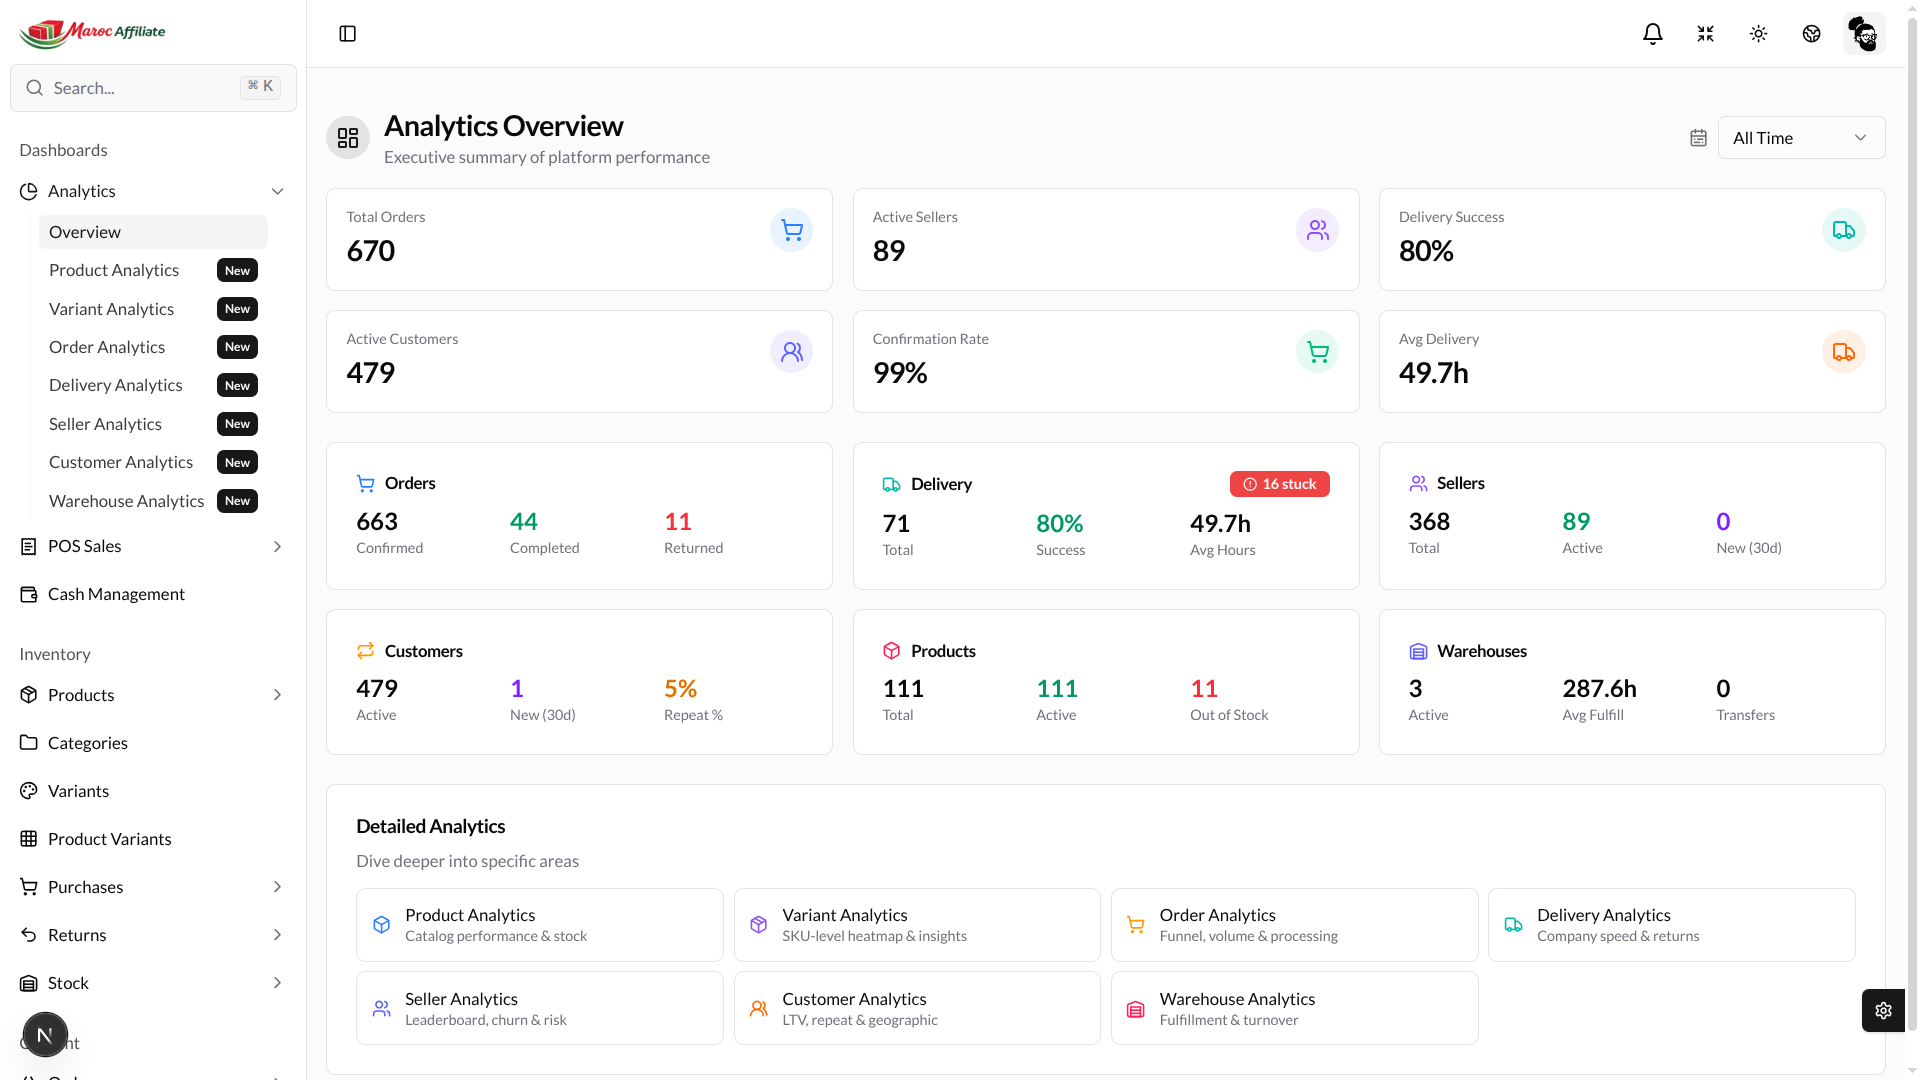
\includegraphics[width=\textwidth]{PFAimages/Screenshot from 2026-05-30 13-18-27.png}
\caption{Vue exécutive -- Cartes KPI agrégées avec indicateurs de tendance période-sur-période}
\end{figure}

\subsubsection{Sous-tableau Commandes}

Le sous-tableau des commandes offre un funnel de conversion complet (de la commande non confirmée jusqu'à la livraison ou le retour) ainsi qu'une analyse géographique permettant d'identifier les villes les plus performantes et celles avec un taux de retour anormal. Le funnel visualise chaque étape du cycle de vie (NOT\_CONFIRMED → CONFIRMED → PROCESSING → IN\_DELIVERY → COMPLETED/RETURNED) avec les taux de conversion inter-étapes et les volumes absolus.

\begin{figure}[H]
\centering
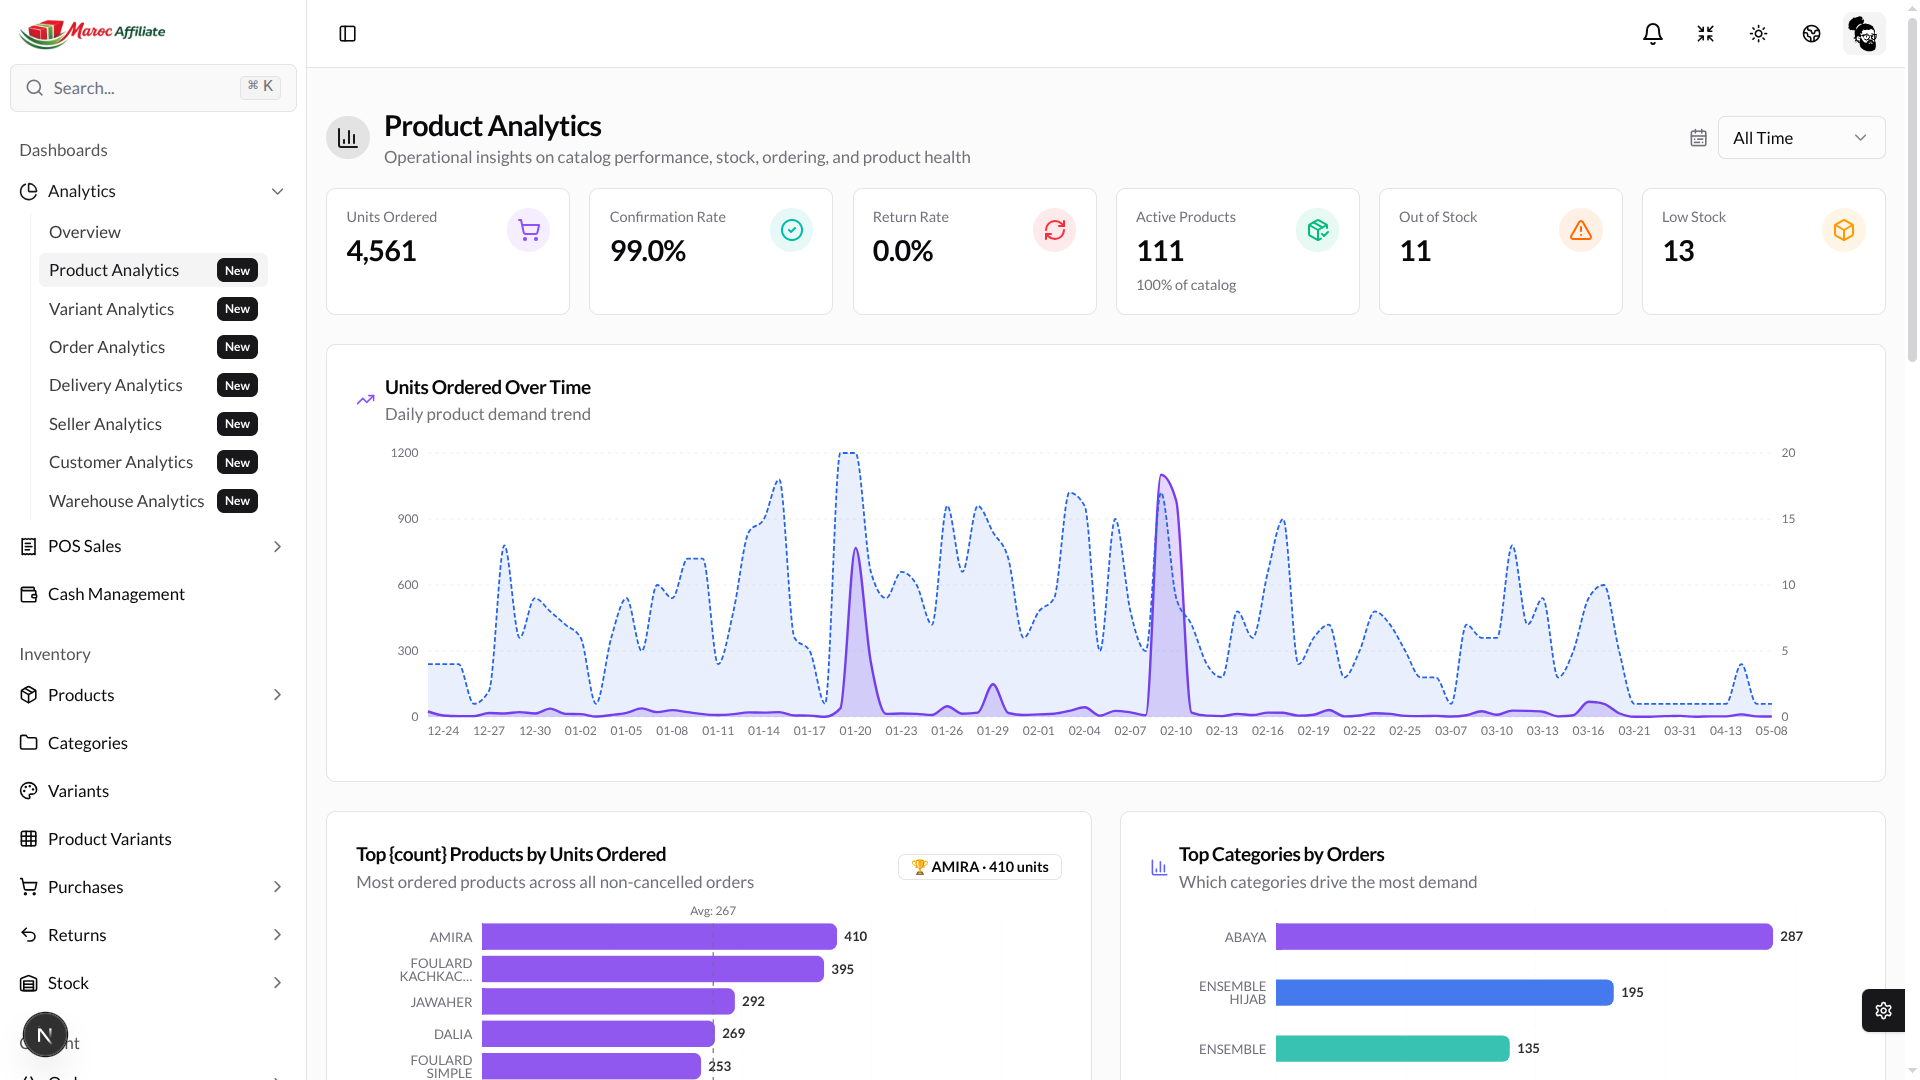
\includegraphics[width=\textwidth]{PFAimages/Screenshot from 2026-05-30 13-19-26.png}
\caption{Analytics Commandes -- Funnel de conversion et tendance de volume temporelle}
\end{figure}

L'analyse par ville croise le volume de commandes avec le taux de confirmation et le taux de retour. Les villes avec un ratio retour/confirmation supérieur à 30\% sont signalées en rouge, permettant d'identifier les zones géographiques problématiques (produits inadaptés à la clientèle locale ou problèmes de livraison récurrents).

\begin{figure}[H]
\centering
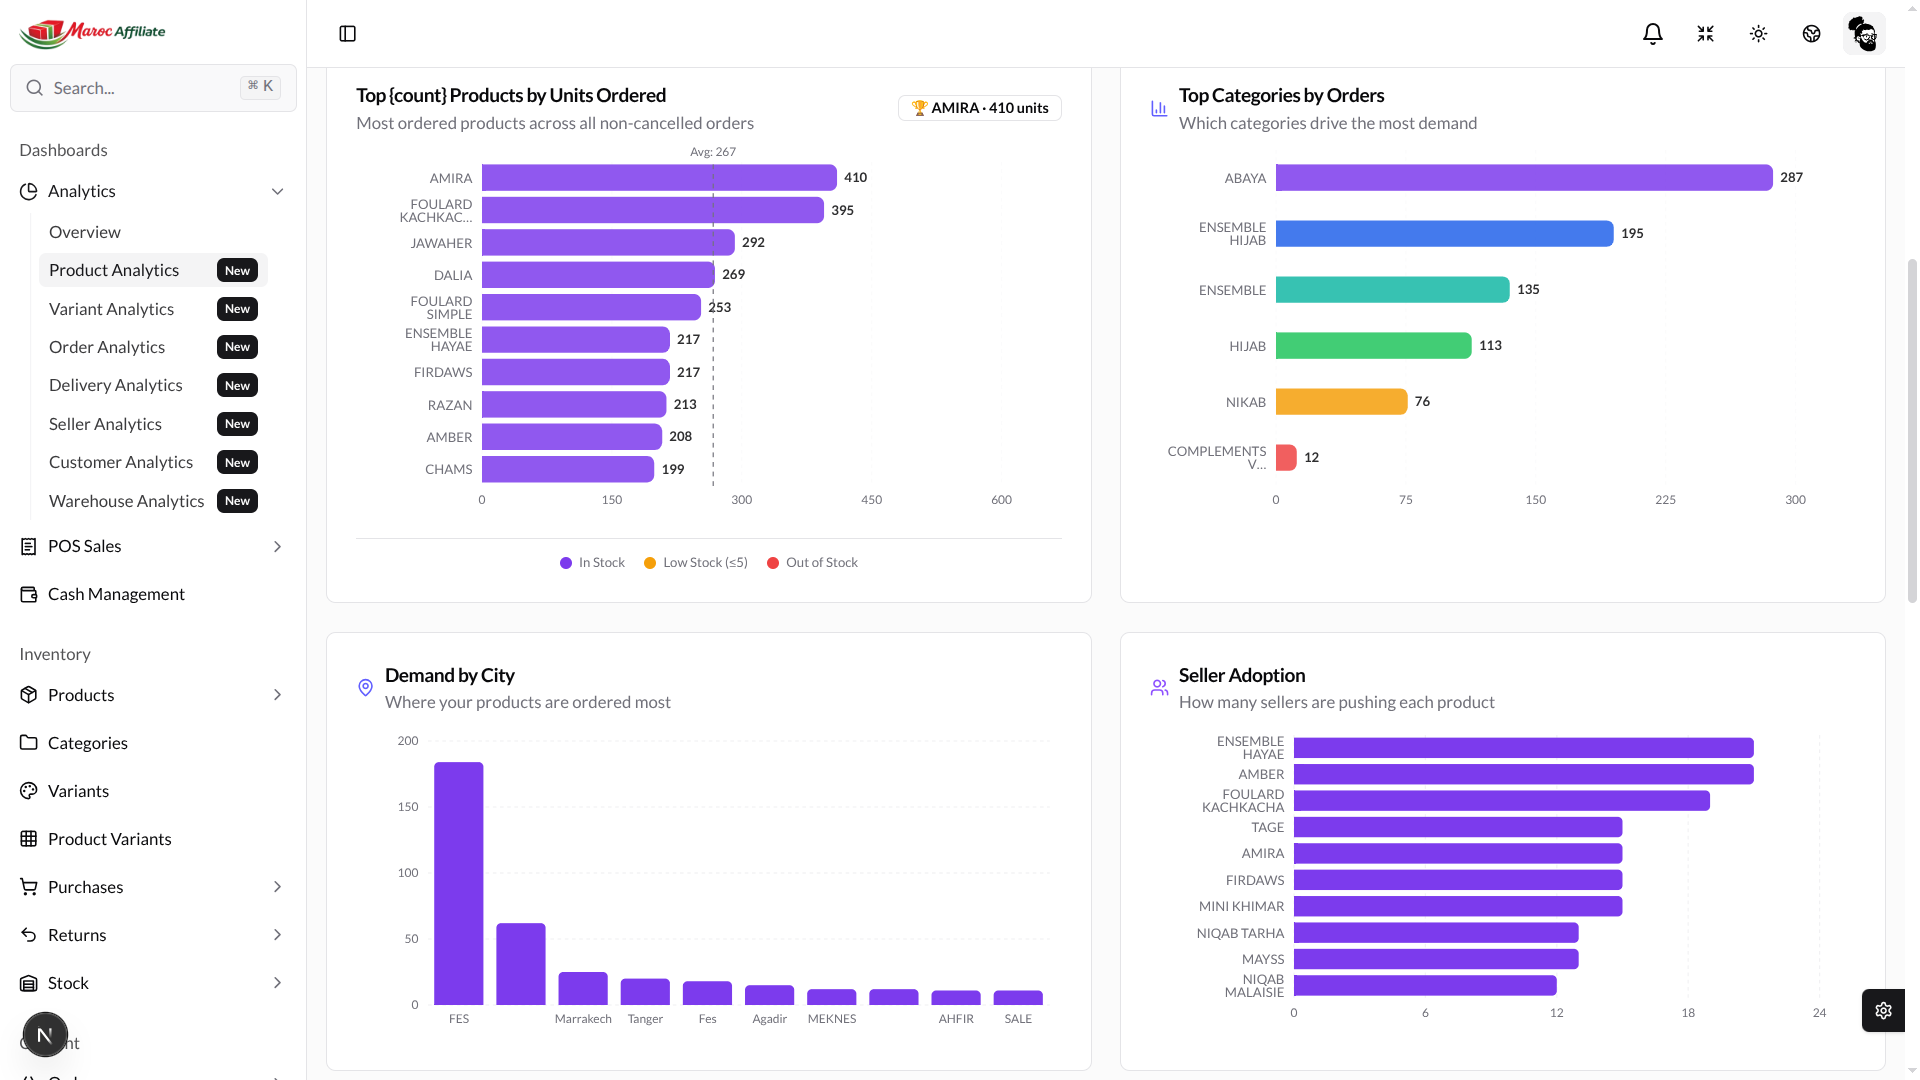
\includegraphics[width=\textwidth]{PFAimages/Screenshot from 2026-05-30 13-19-42.png}
\caption{Analytics Commandes -- Performance par ville avec taux de confirmation et retour}
\end{figure}

Cette vue géographique est particulièrement utile pour les décisions d'expansion : elle révèle les villes à fort potentiel (volume élevé, bon taux de confirmation) et celles où la plateforme rencontre des difficultés structurelles. L'administrateur peut ainsi adapter sa stratégie de livraison ou orienter les vendeurs vers les zones les plus réceptives. Les données sont calculées sur la période sélectionnée et comparées automatiquement à la période précédente pour détecter les évolutions.

\subsubsection{Sous-tableau Livraison}

L'analytics livraison compare les performances des sociétés de transport sur plusieurs axes : taux de succès, délai moyen, et raisons de retour. L'alerte « livraisons bloquées » identifie automatiquement les colis sans mouvement depuis plus de 48 heures, permettant une intervention rapide auprès du transporteur concerné.

\begin{figure}[H]
\centering
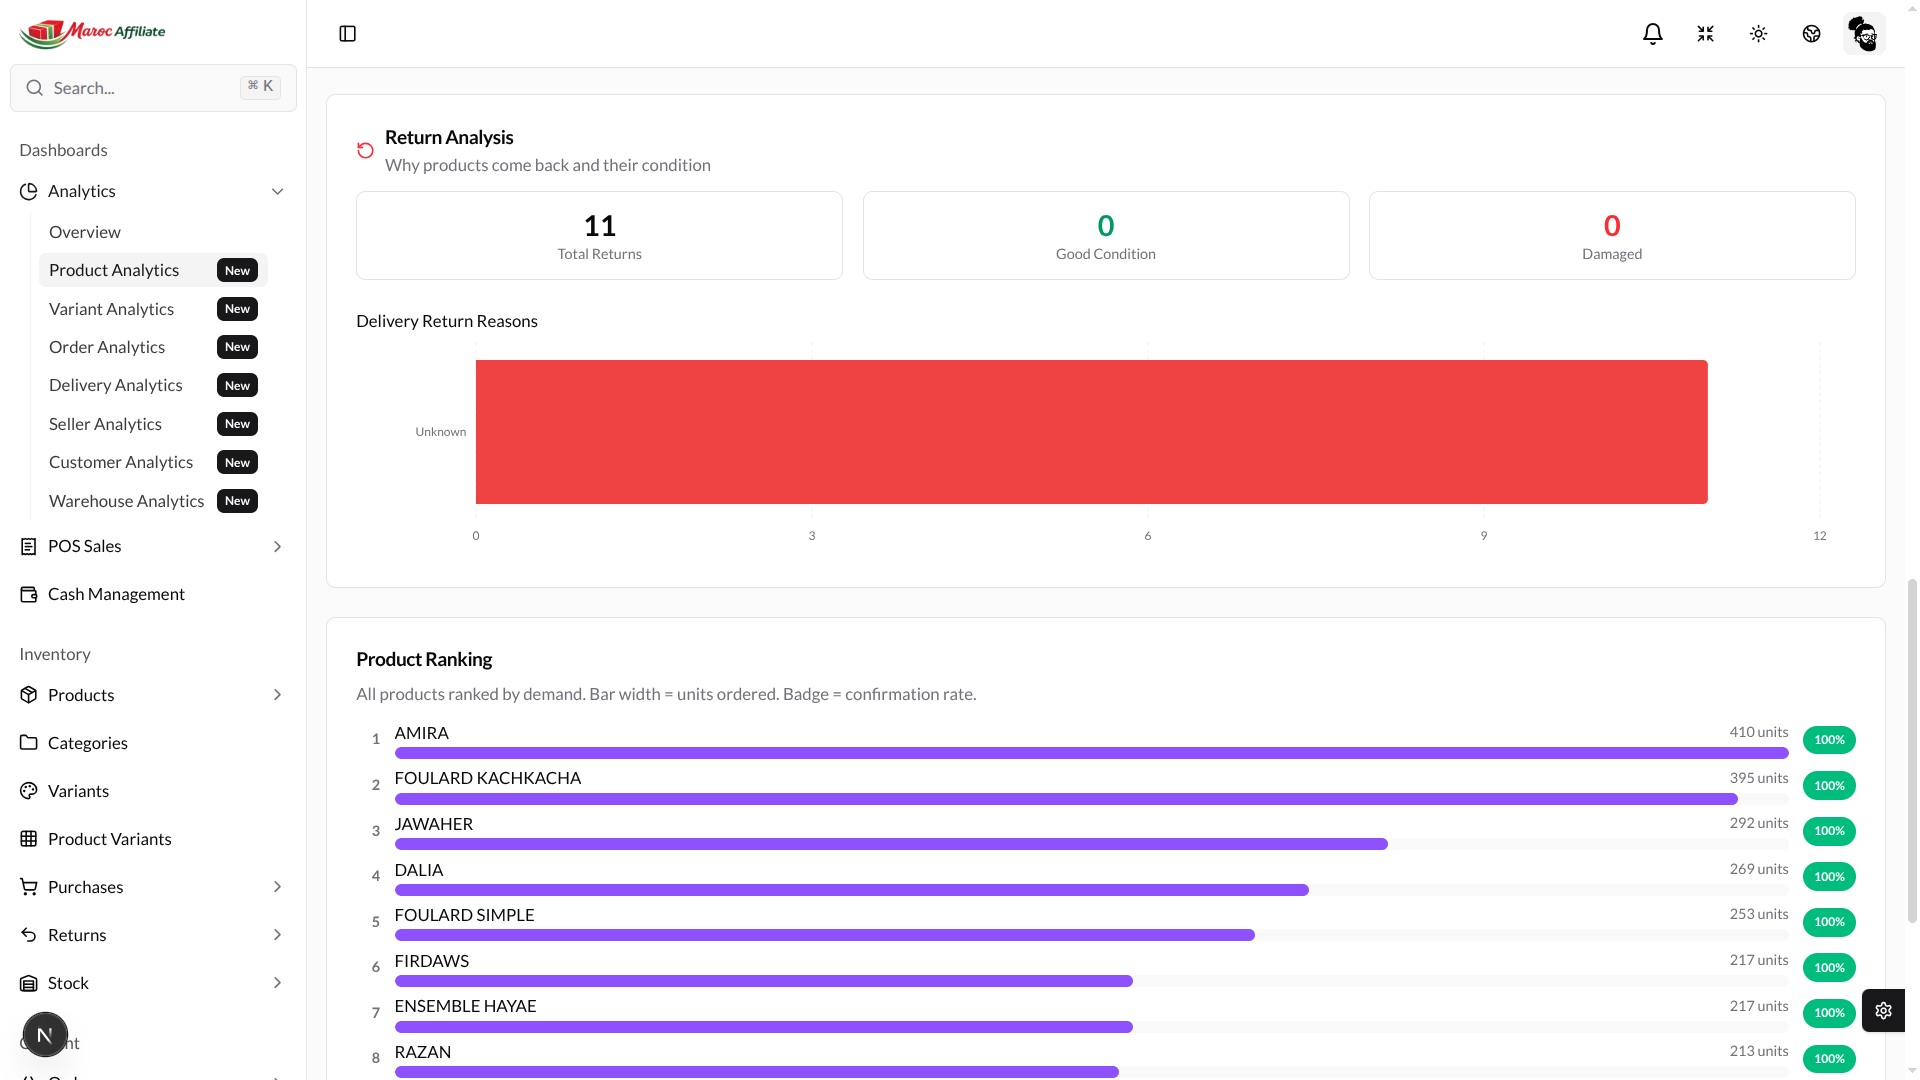
\includegraphics[width=\textwidth]{PFAimages/Screenshot from 2026-05-30 13-19-51.png}
\caption{Analytics Livraison -- Comparaison des transporteurs par taux de succès et délai}
\end{figure}

La décomposition des délais distingue le temps de prise en charge (confirmation → expédition), le temps de transit, et le temps de livraison finale. Cette granularité permet d'identifier précisément le goulot d'étranglement dans la chaîne logistique. Les motifs de retour sont catégorisés (refus client, adresse incorrecte, absence, colis endommagé) pour alimenter les décisions d'optimisation.

\begin{figure}[H]
\centering
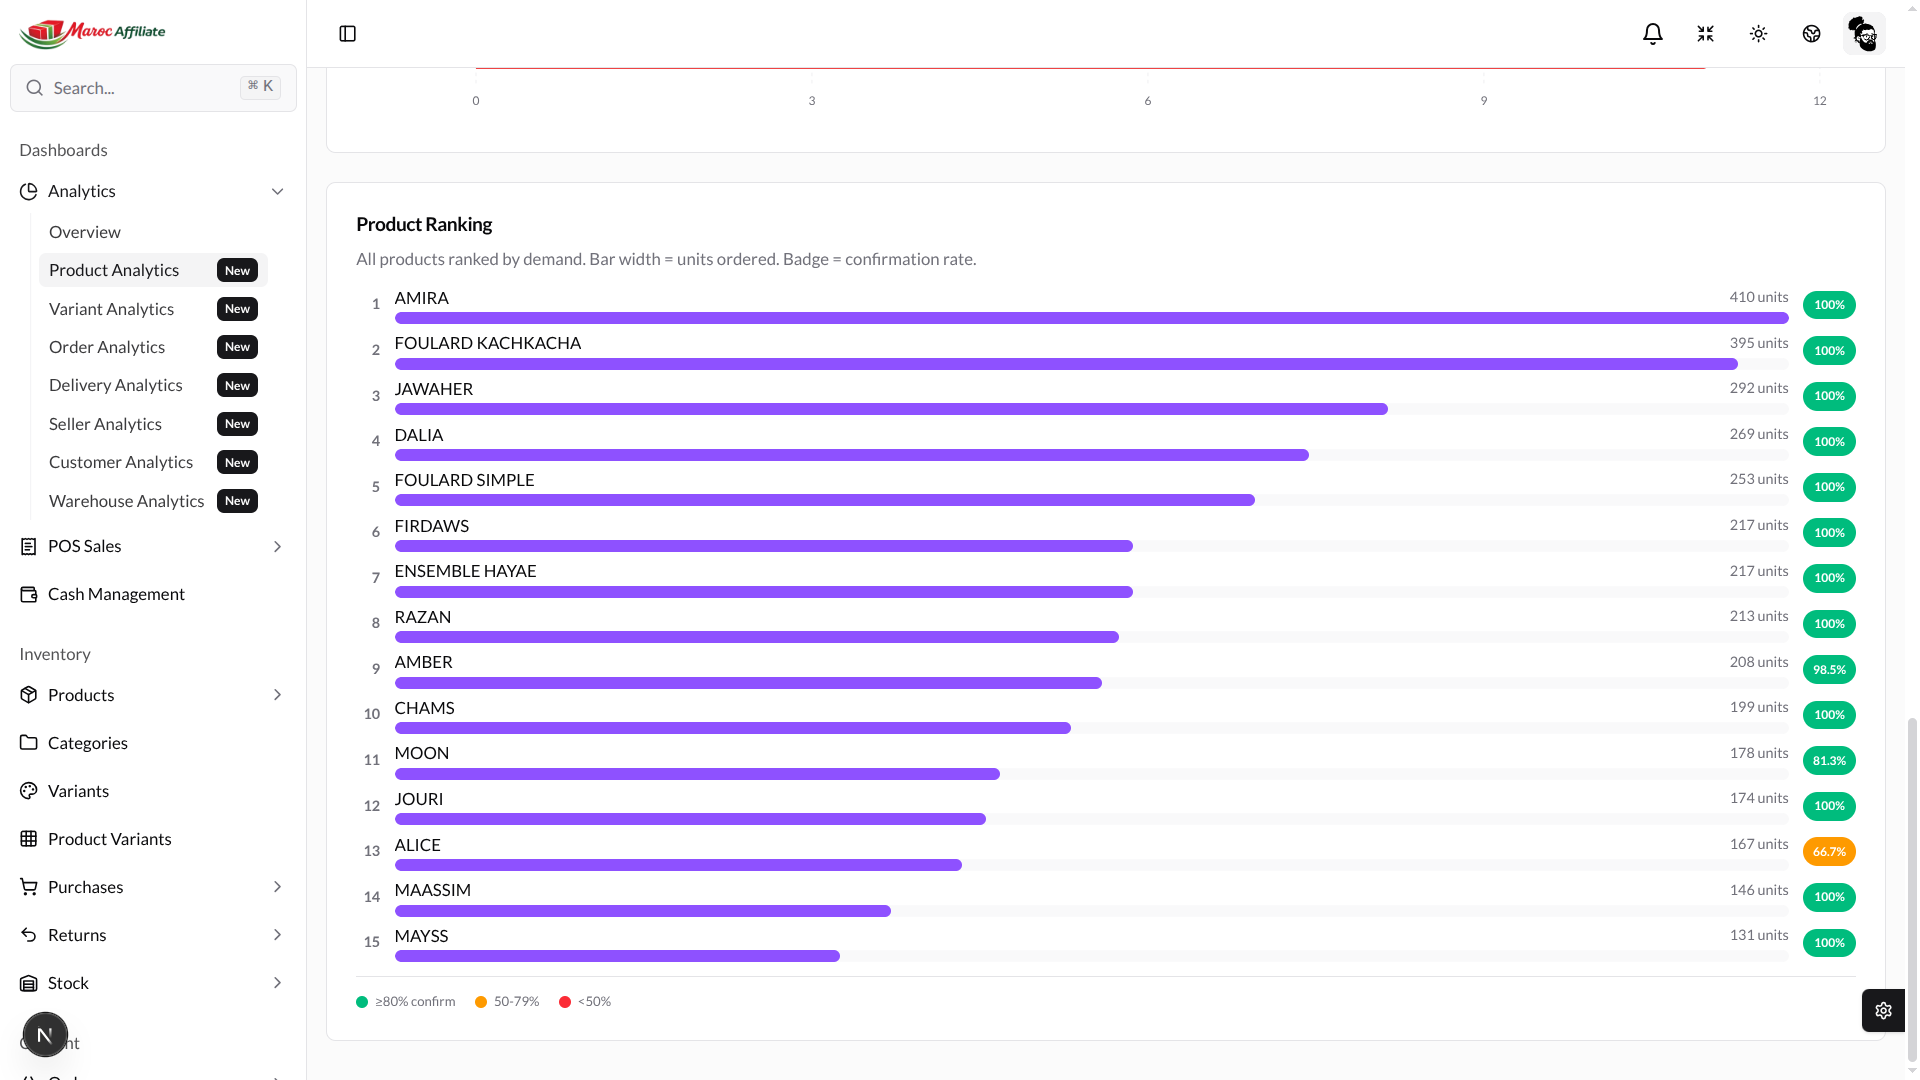
\includegraphics[width=\textwidth]{PFAimages/Screenshot from 2026-05-30 13-19-54.png}
\caption{Analytics Livraison -- Décomposition des délais et distribution des motifs de retour}
\end{figure}

Ces indicateurs permettent de prendre des décisions concrètes : renégocier un contrat avec un transporteur sous-performant, ajuster les zones de couverture, ou identifier les créneaux horaires où le taux de réussite est le plus élevé. Les données alimentent également le système d'alertes automatiques qui notifie l'administration lorsqu'un transporteur dépasse le seuil de 20\% de retours sur une fenêtre glissante de 7 jours.

\subsubsection{Sous-tableaux Produits et Variantes}

Le quadrant produit croise la performance commerciale avec le niveau de stock pour identifier quatre catégories : stars (haute performance, bon stock), opportunités (bonne performance, stock faible), surstock (faible performance, stock élevé), et dormants (faible sur les deux axes).

\begin{figure}[H]
\centering
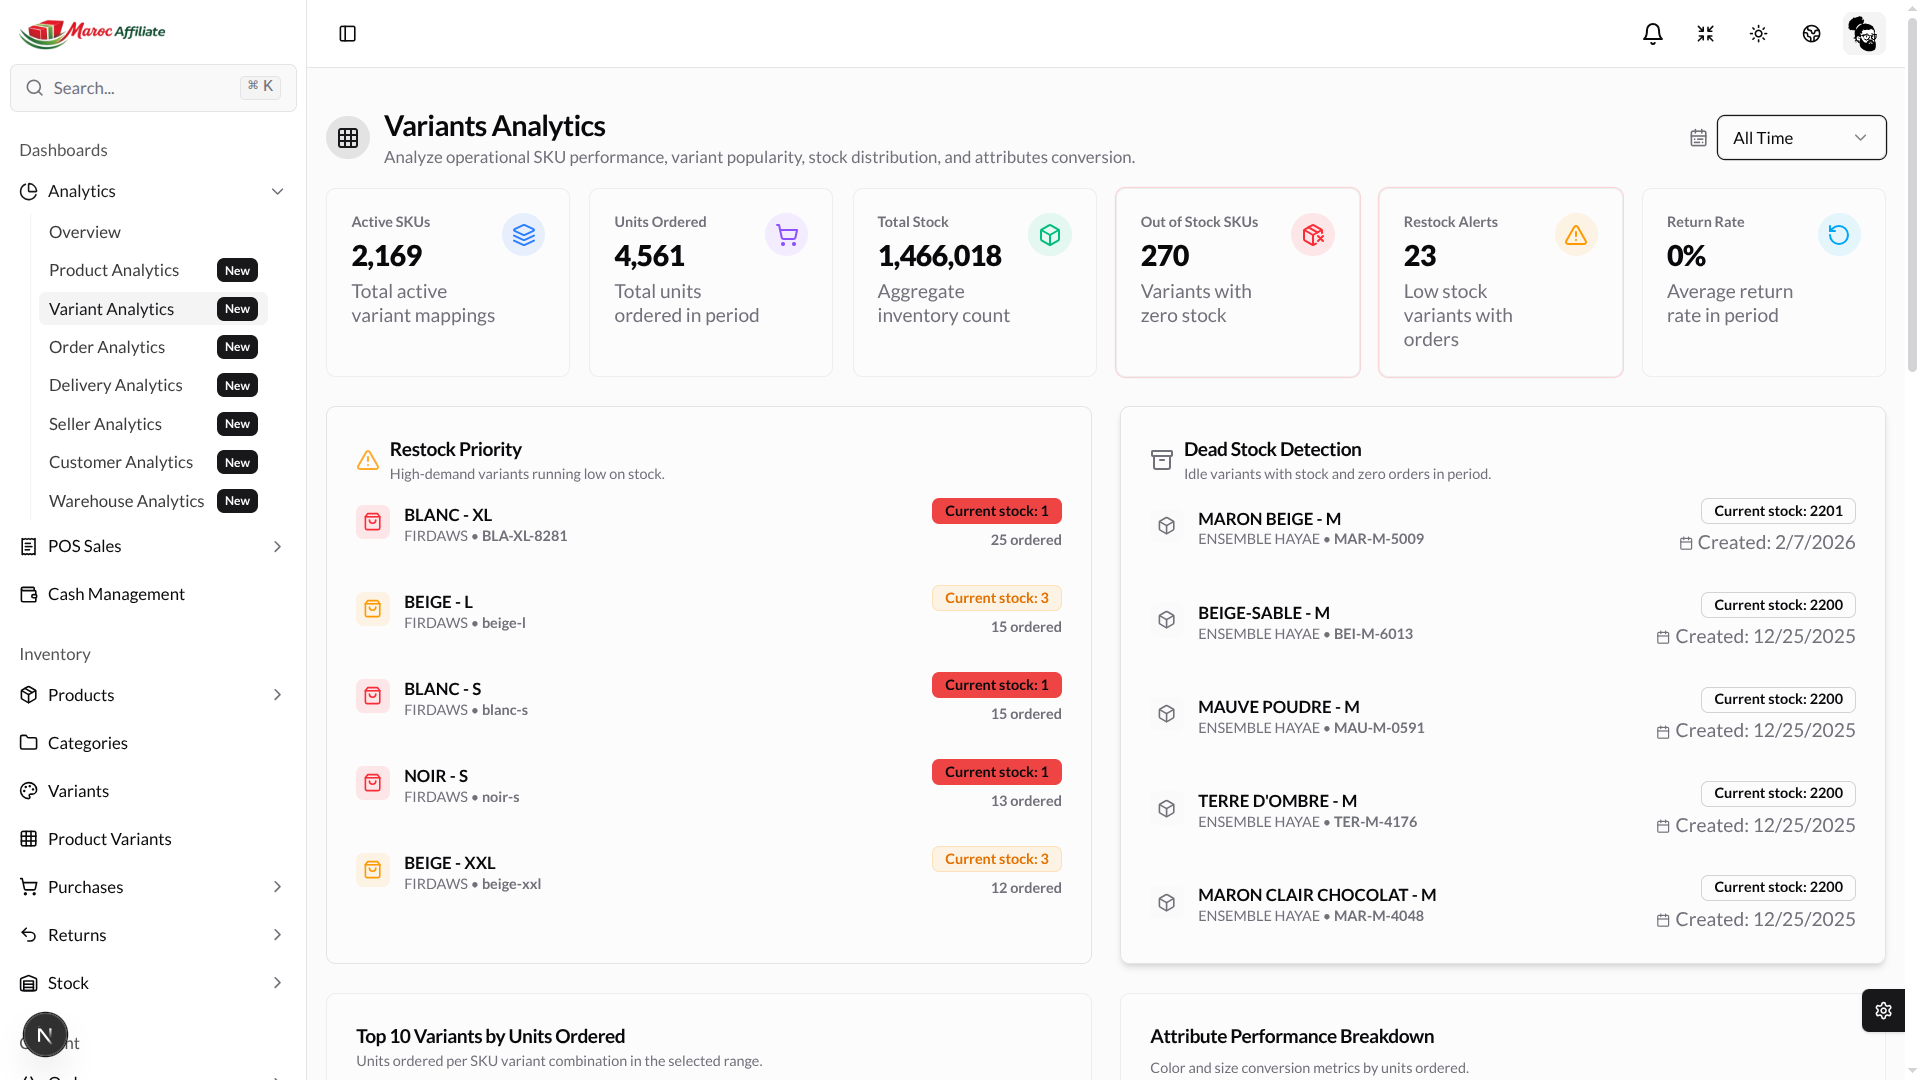
\includegraphics[width=\textwidth]{PFAimages/Screenshot from 2026-05-30 13-20-12.png}
\caption{Analytics Produits -- Quadrant performance vs stock pour prioriser les actions}
\end{figure}

La heatmap des variantes permet de visualiser en un coup d'œil quelles combinaisons couleur/taille se vendent le mieux, sont en rupture, ou présentent un taux de retour élevé.

\begin{figure}[H]
\centering
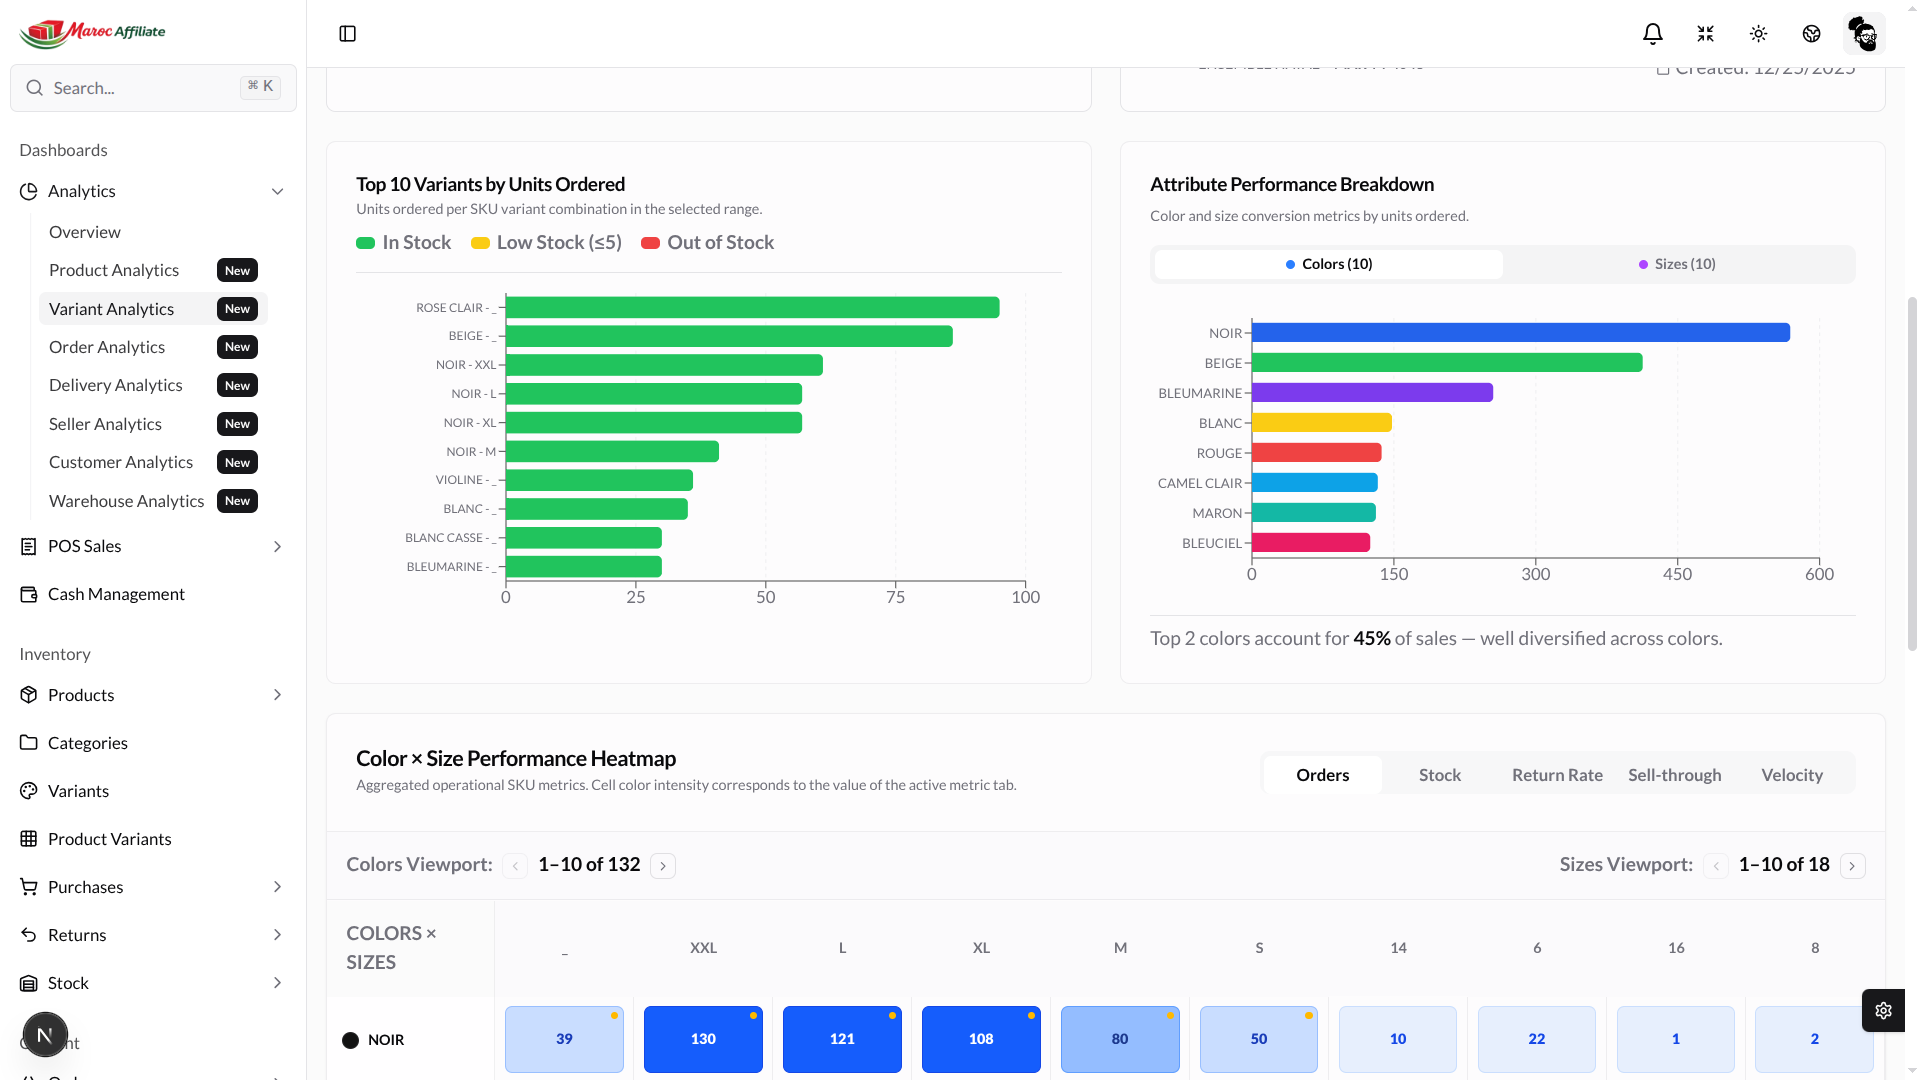
\includegraphics[width=\textwidth]{PFAimages/Screenshot from 2026-05-30 13-20-19.png}
\caption{Analytics Variantes -- Heatmap couleur $\times$ taille avec 5 modes d'affichage}
\end{figure}

La heatmap offre 5 modes d'affichage sélectionnables : \textbf{Quantity} (unités vendues par combinaison), \textbf{Revenue} (chiffre d'affaires), \textbf{Stock} (niveau de stock actuel), \textbf{Returns} (taux de retour) et \textbf{Velocity} (vitesse d'écoulement). Le graphique horizontal à gauche (\textit{Top All Variations by Order Ordered}) classe les variantes par volume de commandes, distinguant les statuts (Stock, Listed Below Cost, Out of Stock). À droite, le graphique \textit{Attribute Performance Breakdown} compare les performances par attribut (couleur ou taille) en termes de ventes et de revenue, permettant d'identifier rapidement les attributs les plus rentables et ceux nécessitant un réassort.

\subsubsection{Sous-tableau Vendeurs (Seller Analytics)}

Le sous-tableau vendeurs est dédié au suivi de la performance commerciale des affiliés. Il présente en haut cinq cartes KPI : le nombre total de vendeurs inscrits (368), les vendeurs actifs sur la période (85), les nouveaux vendeurs (derniers 30 jours), le nombre moyen de commandes par vendeur (7.6), et les charges de responsabilité (liability charges pour les force-confirm abusifs).

Le graphique \textbf{Seller Activity Trend} affiche deux séries temporelles superposées : le nombre de commandes quotidiennes (vert) et le nombre de vendeurs actifs distincts (bleu). Cette visualisation permet de détecter les jours de forte activité et d'identifier les tendances de participation des vendeurs.

En dessous, le \textbf{Seller Leaderboard} classe les vendeurs par profit total généré (bénéfice = prix de vente - coût - frais de livraison), avec le nombre de commandes et le taux de succès (pourcentage de commandes complétées vs retournées). Ce classement permet d'identifier les top performers mais aussi les vendeurs avec un taux de succès anormalement bas (< 50\%, affiché en rouge).

\begin{figure}[H]
\centering
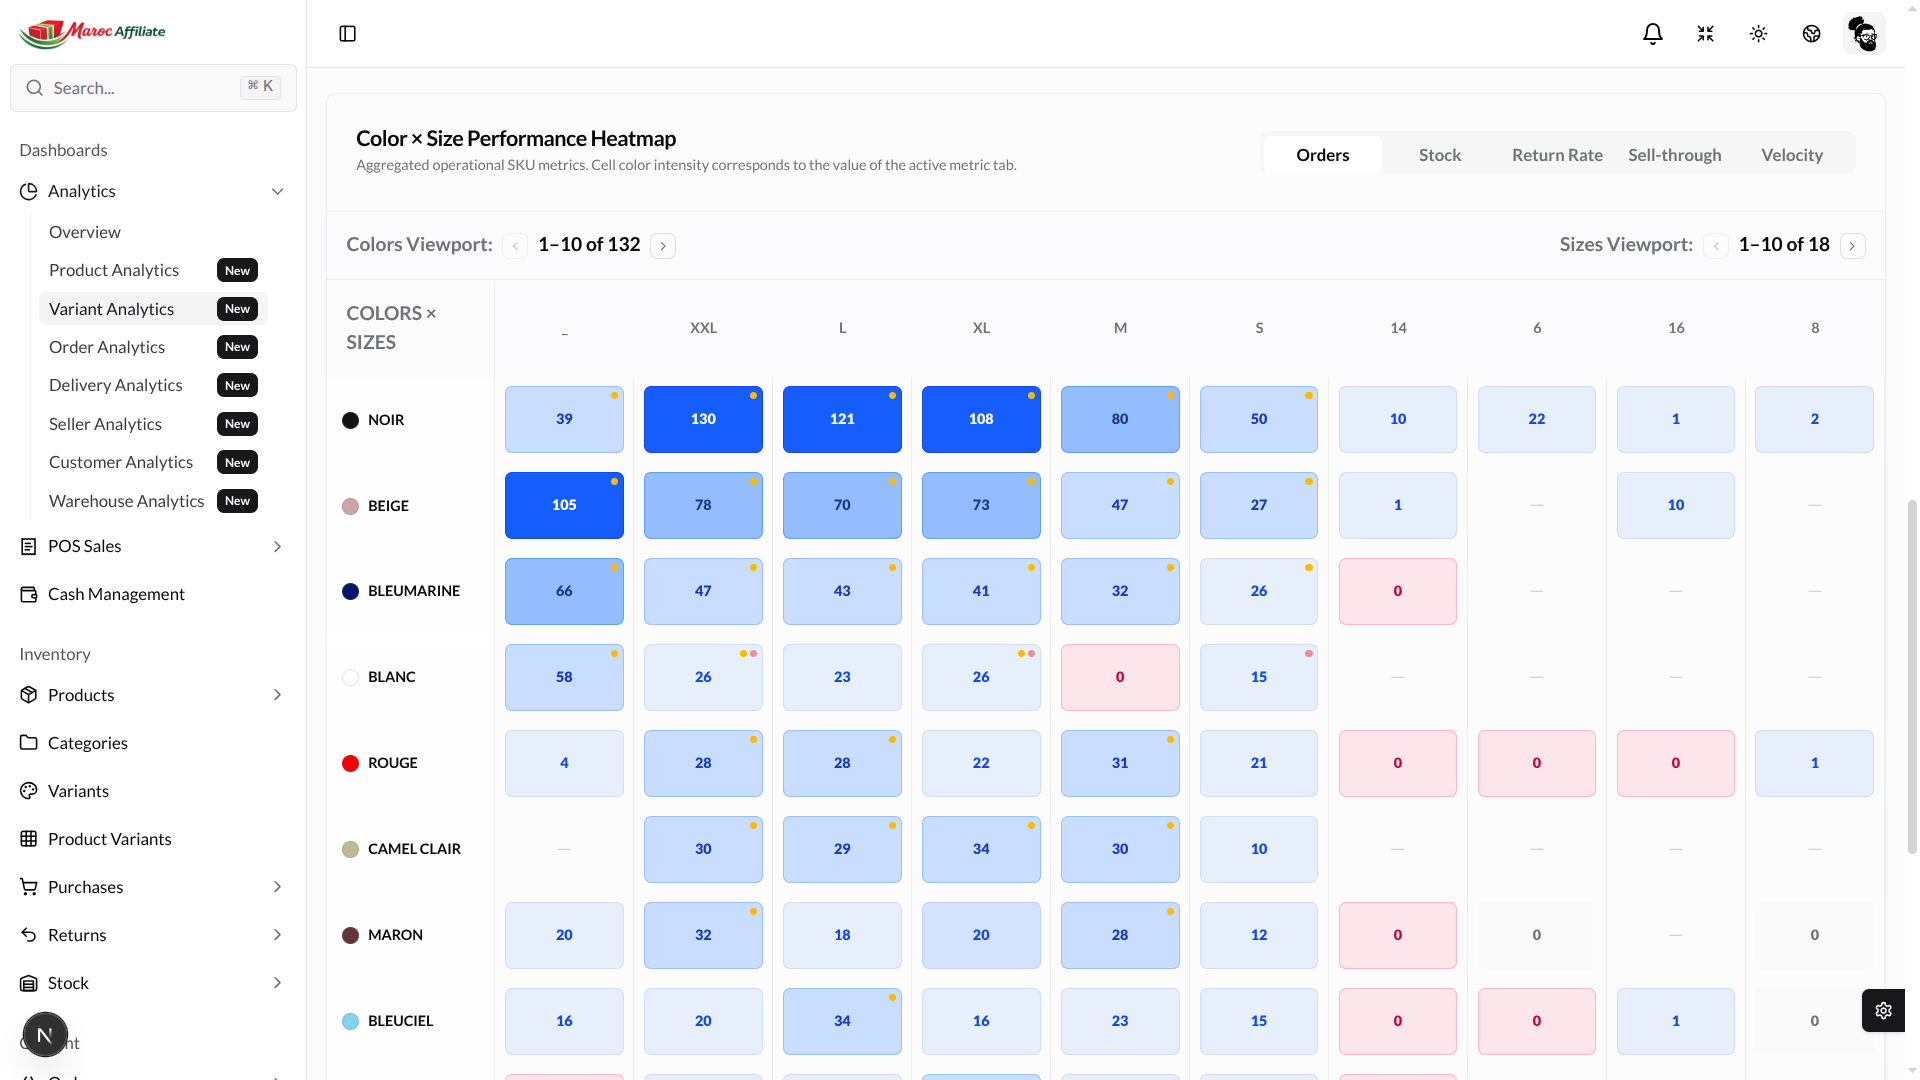
\includegraphics[width=\textwidth]{PFAimages/Screenshot from 2026-05-30 13-20-28.png}
\caption{Seller Analytics -- KPIs, tendance d'activité quotidienne, et leaderboard par profit}
\end{figure}

Le leaderboard identifie également les vendeurs présentant un taux de succès critique (< 50\%), signalé en rouge. Ce seuil d'alerte permet à l'administration de déclencher un accompagnement ciblé ou d'ajuster les conditions de force-confirm pour ces profils. La corrélation entre le volume de commandes et le taux de succès constitue un indicateur avancé de la qualité du réseau d'affiliés.

\subsubsection{Sous-tableau Clients (Customer Analytics)}

L'analytics clients segmente la base de clients selon leur valeur vie (LTV) en quatre tranches : clients à commande unique (1), clients récurrents légers (2--3), clients réguliers (4--6), et clients fidèles (7+). Cette segmentation permet de mesurer le taux de rétention et d'identifier les leviers de fidélisation.

Le module inclut également l'analyse géographique de la demande (villes avec le plus de clients actifs), le suivi des tendances de mise en liste noire (blacklist), et l'attribution par vendeur (quel affilié amène le plus de nouveaux clients à la plateforme).

\begin{figure}[H]
\centering
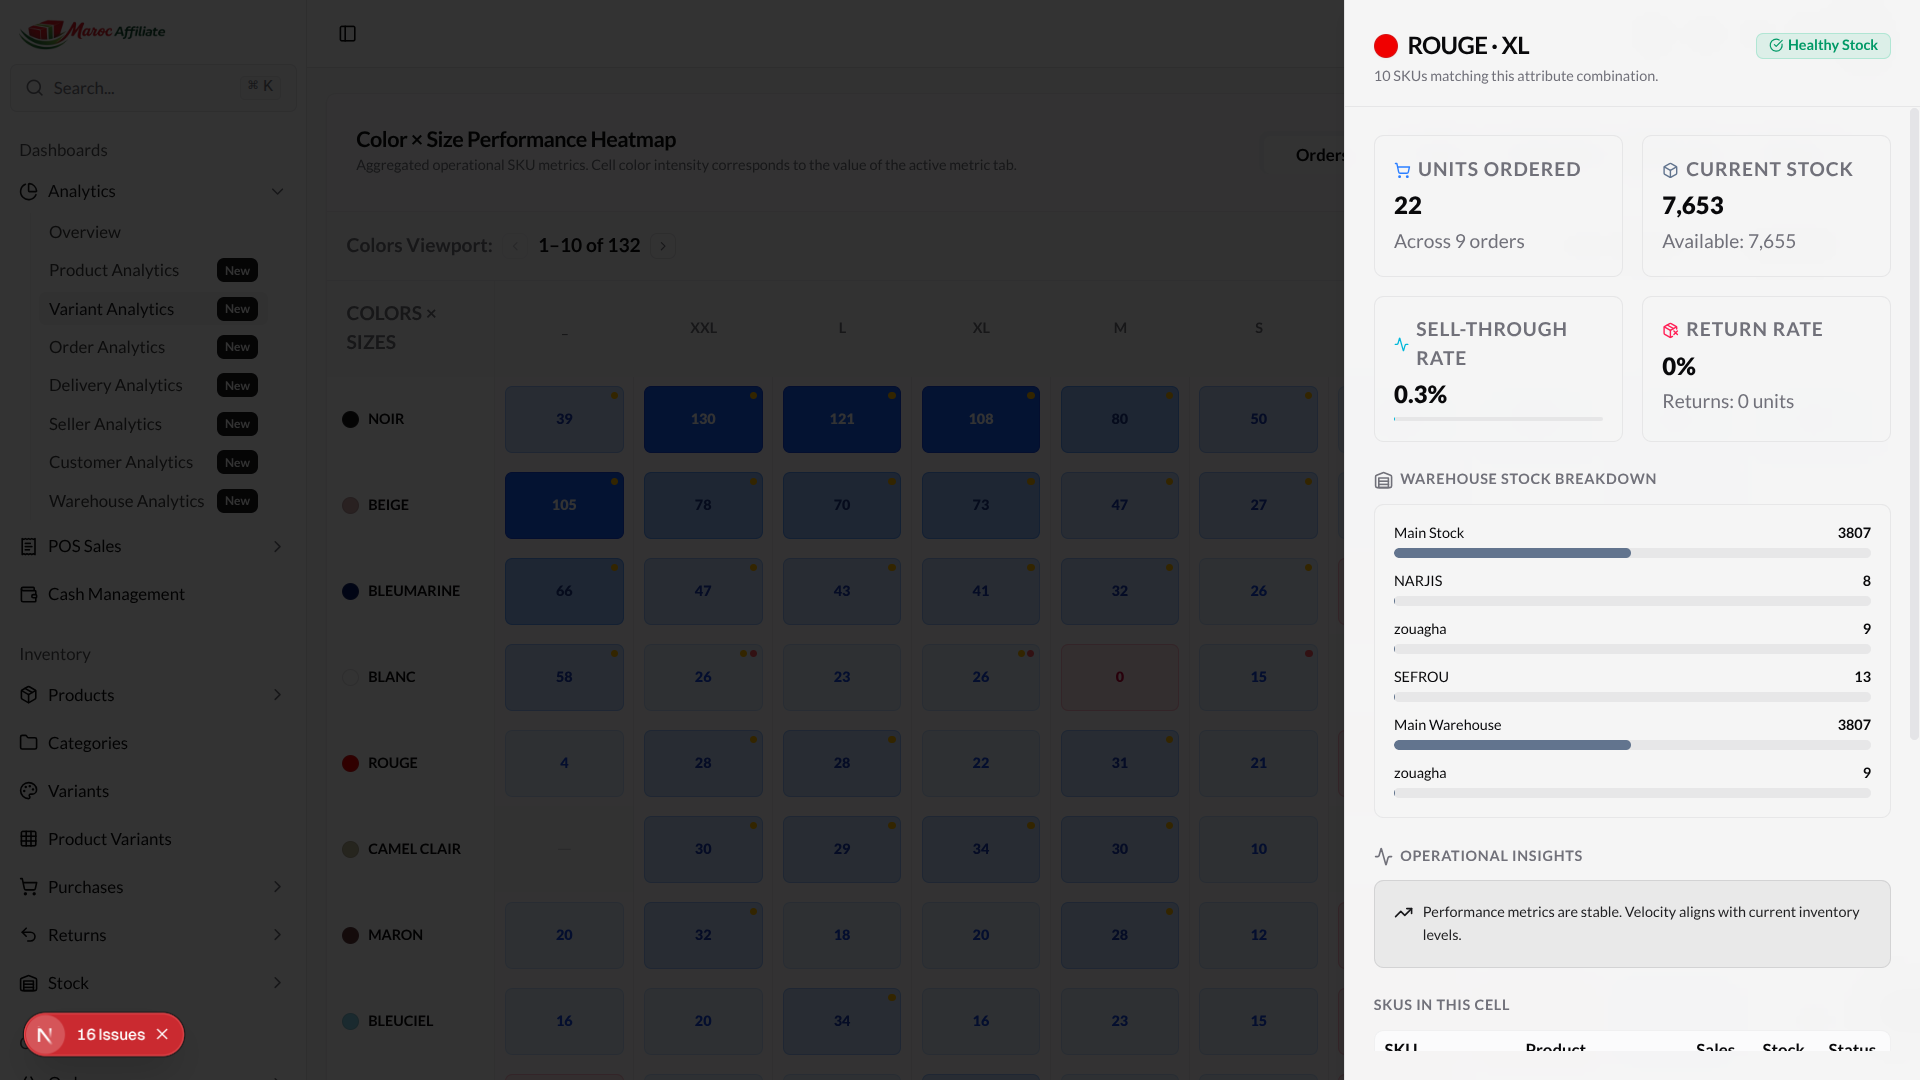
\includegraphics[width=\textwidth]{PFAimages/Screenshot from 2026-05-30 13-21-59.png}
\caption{Customer Analytics -- Segmentation LTV, analyse de répétition, et demande géographique}
\end{figure}

\subsubsection{Sous-tableau Entrepôts (Warehouse Analytics)}

Le sous-tableau entrepôts permet la comparaison multi-critères entre les différents points de fulfillment. Pour chaque entrepôt, le système calcule : le nombre de commandes fulfillées, le délai moyen de traitement (de la confirmation à l'expédition), le taux de rotation du stock, les ventes POS (point de vente physique), et l'activité de transferts (entrées/sorties).

Cette vue permet d'identifier les entrepôts sous-performants (délai de fulfillment élevé) ou surchargés (stock mort, faible rotation), et d'optimiser la répartition des stocks entre les différents sites.

\begin{figure}[H]
\centering
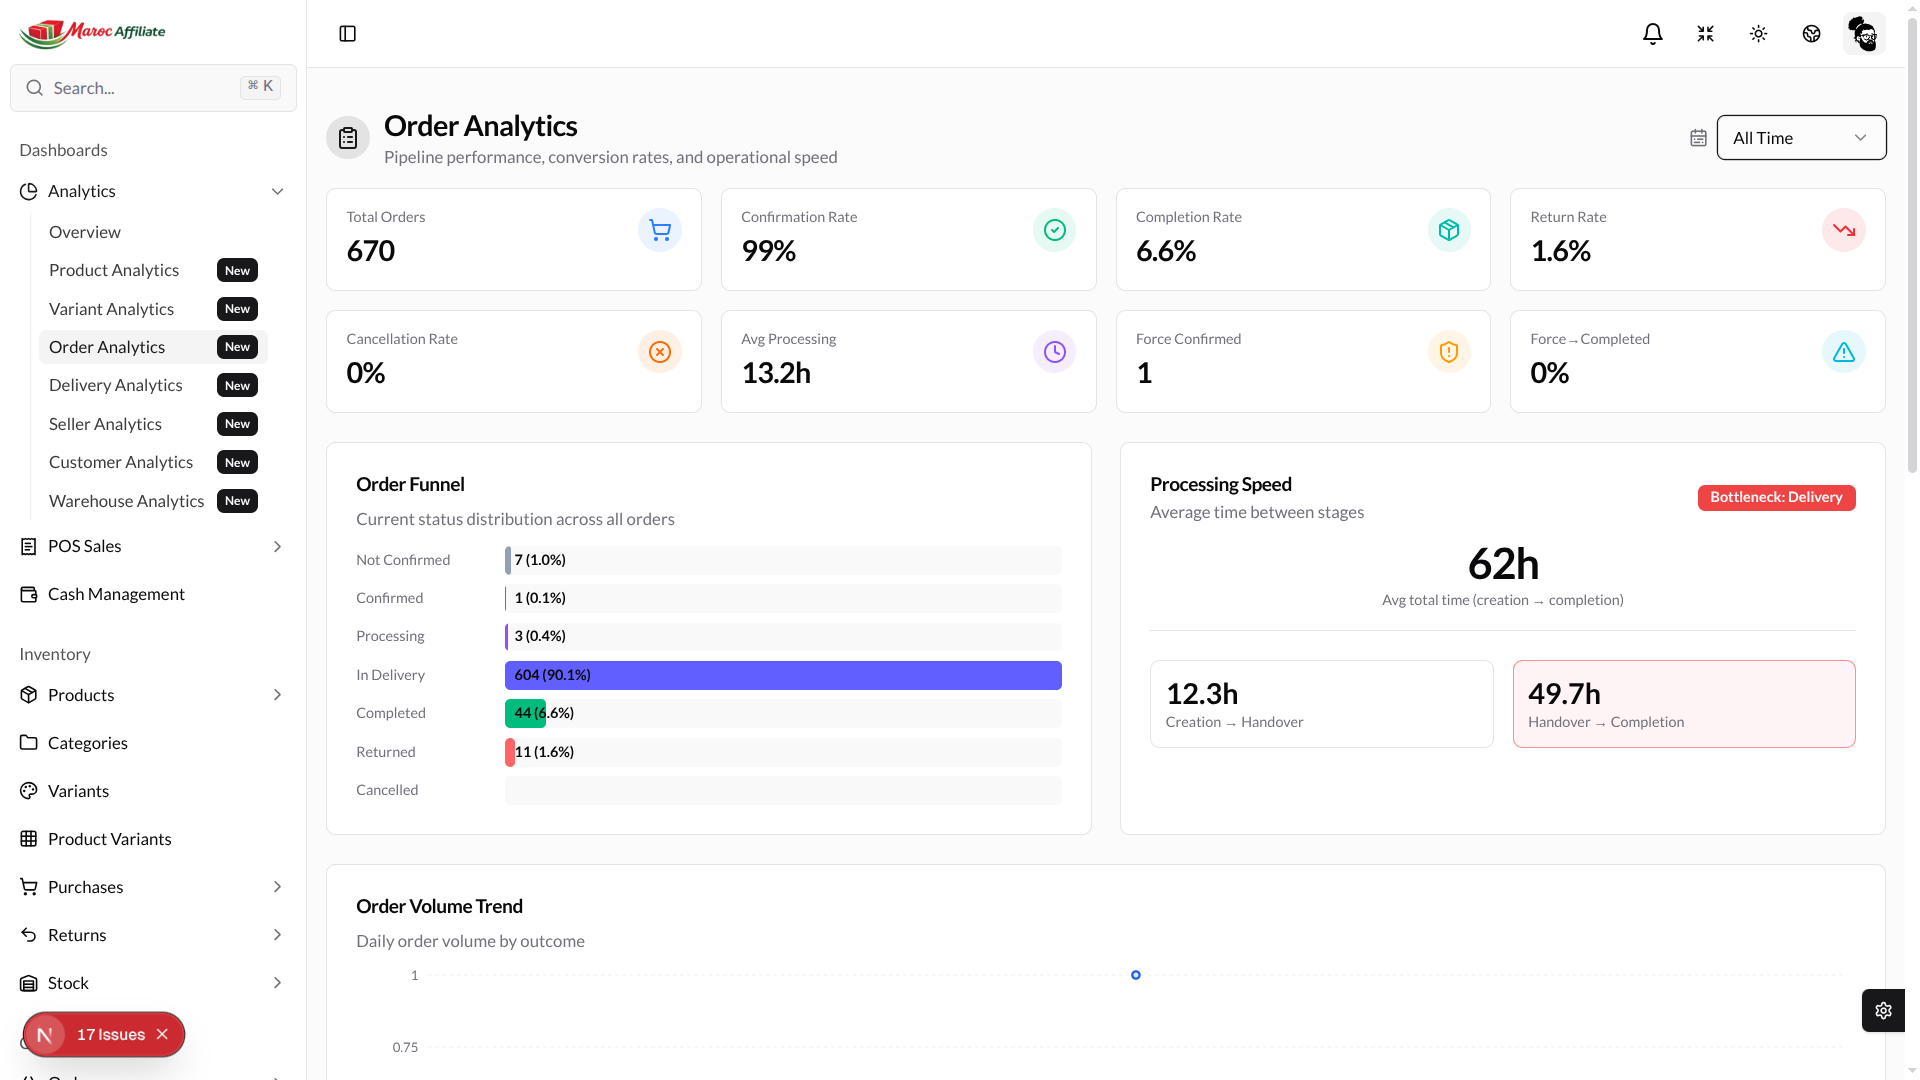
\includegraphics[width=\textwidth]{PFAimages/Screenshot from 2026-05-30 13-22-22.png}
\caption{Warehouse Analytics -- Comparaison multi-critères par entrepôt (fulfillment, stock, POS)}
\end{figure}

\subsubsection{Vues complémentaires de gestion}

Les figures suivantes illustrent d'autres surfaces du dashboard administrateur qui bénéficient des mêmes patterns architecturaux (Server Components, cache, i18n) développés pour le module analytics. Ces vues démontrent la réutilisabilité du système de composants : le \code{DataTable} générique, les filtres combinables, et les panels de détail sont instanciés par simple configuration sans duplication de code.

\begin{figure}[H]
\centering
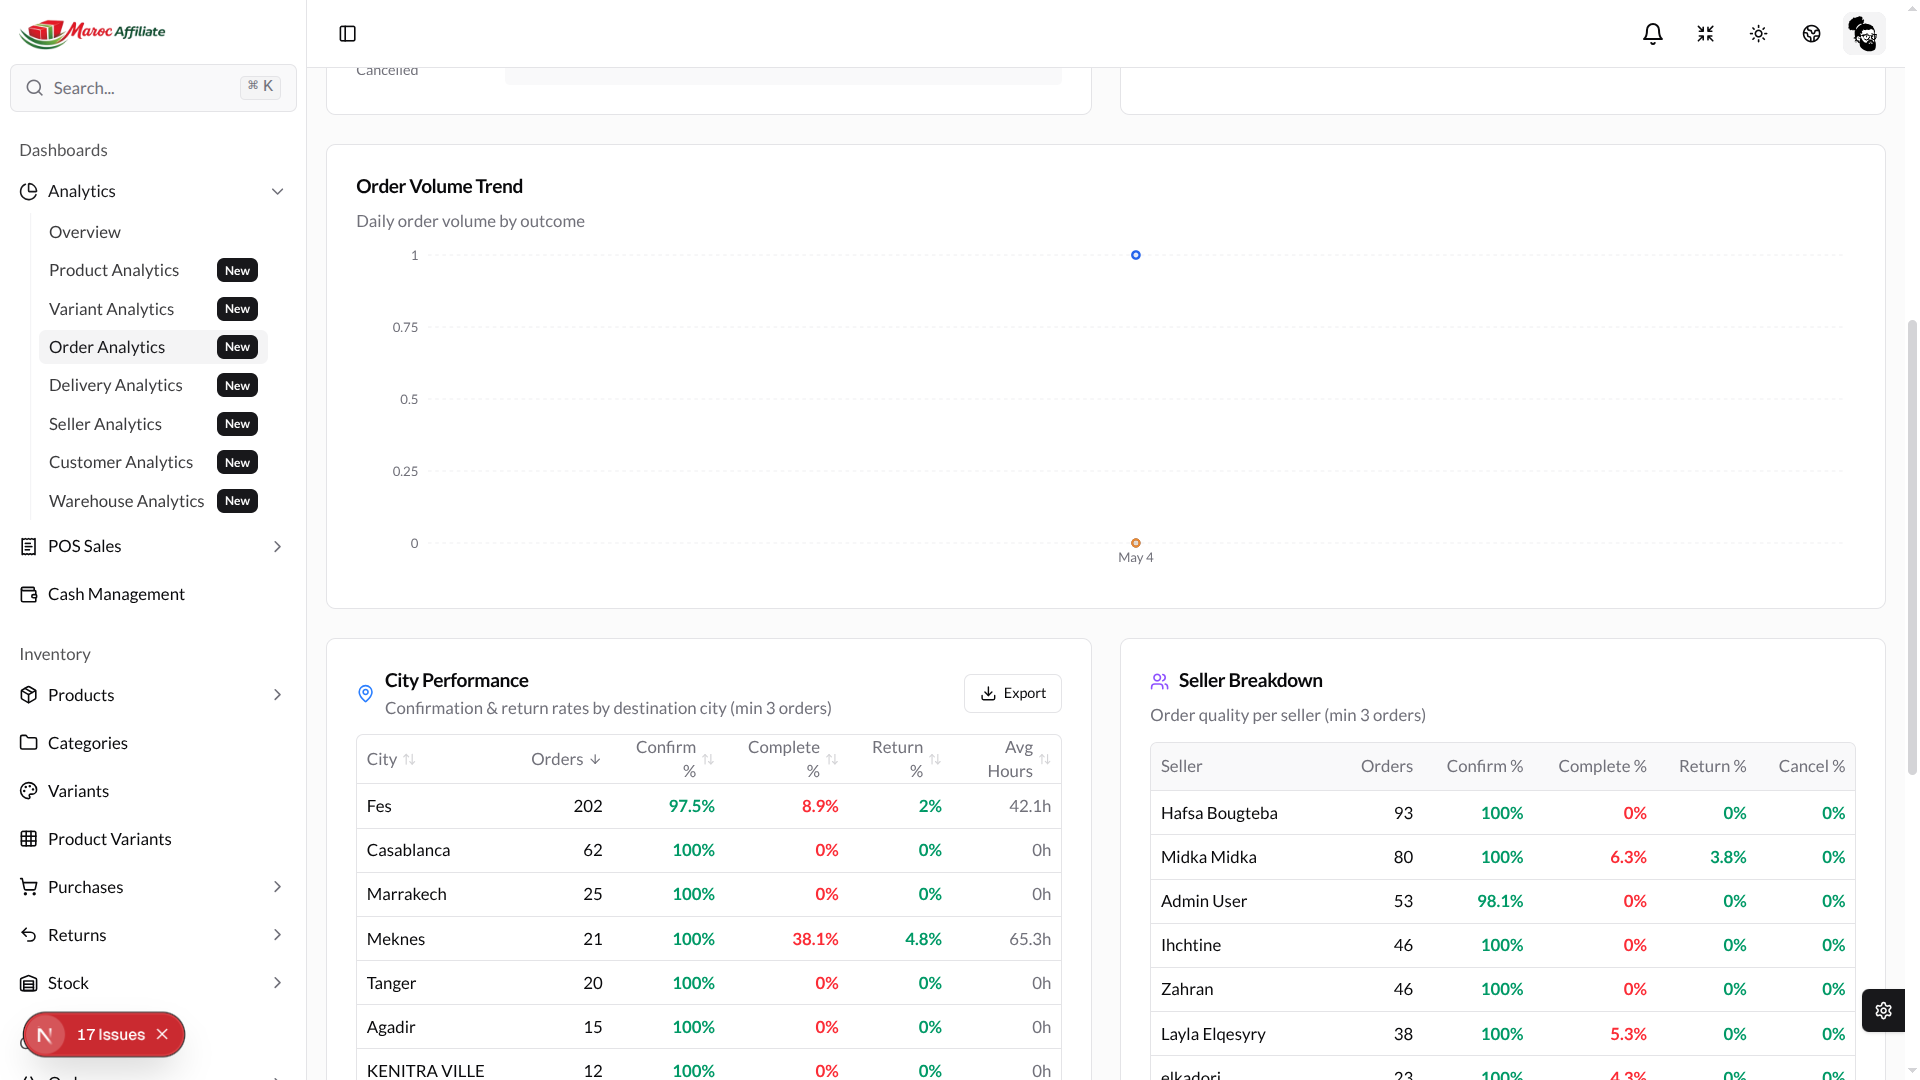
\includegraphics[width=\textwidth]{PFAimages/Screenshot from 2026-05-30 13-22-30.png}
\caption{Dashboard Admin -- Interface de gestion avec DataTable paginée côté serveur}
\end{figure}

La DataTable utilise TanStack Table en mode headless avec pagination, tri et filtrage côté serveur. Les colonnes sont configurées déclarativement et supportent le rendu conditionnel selon les permissions de l'utilisateur connecté.

\begin{figure}[H]
\centering
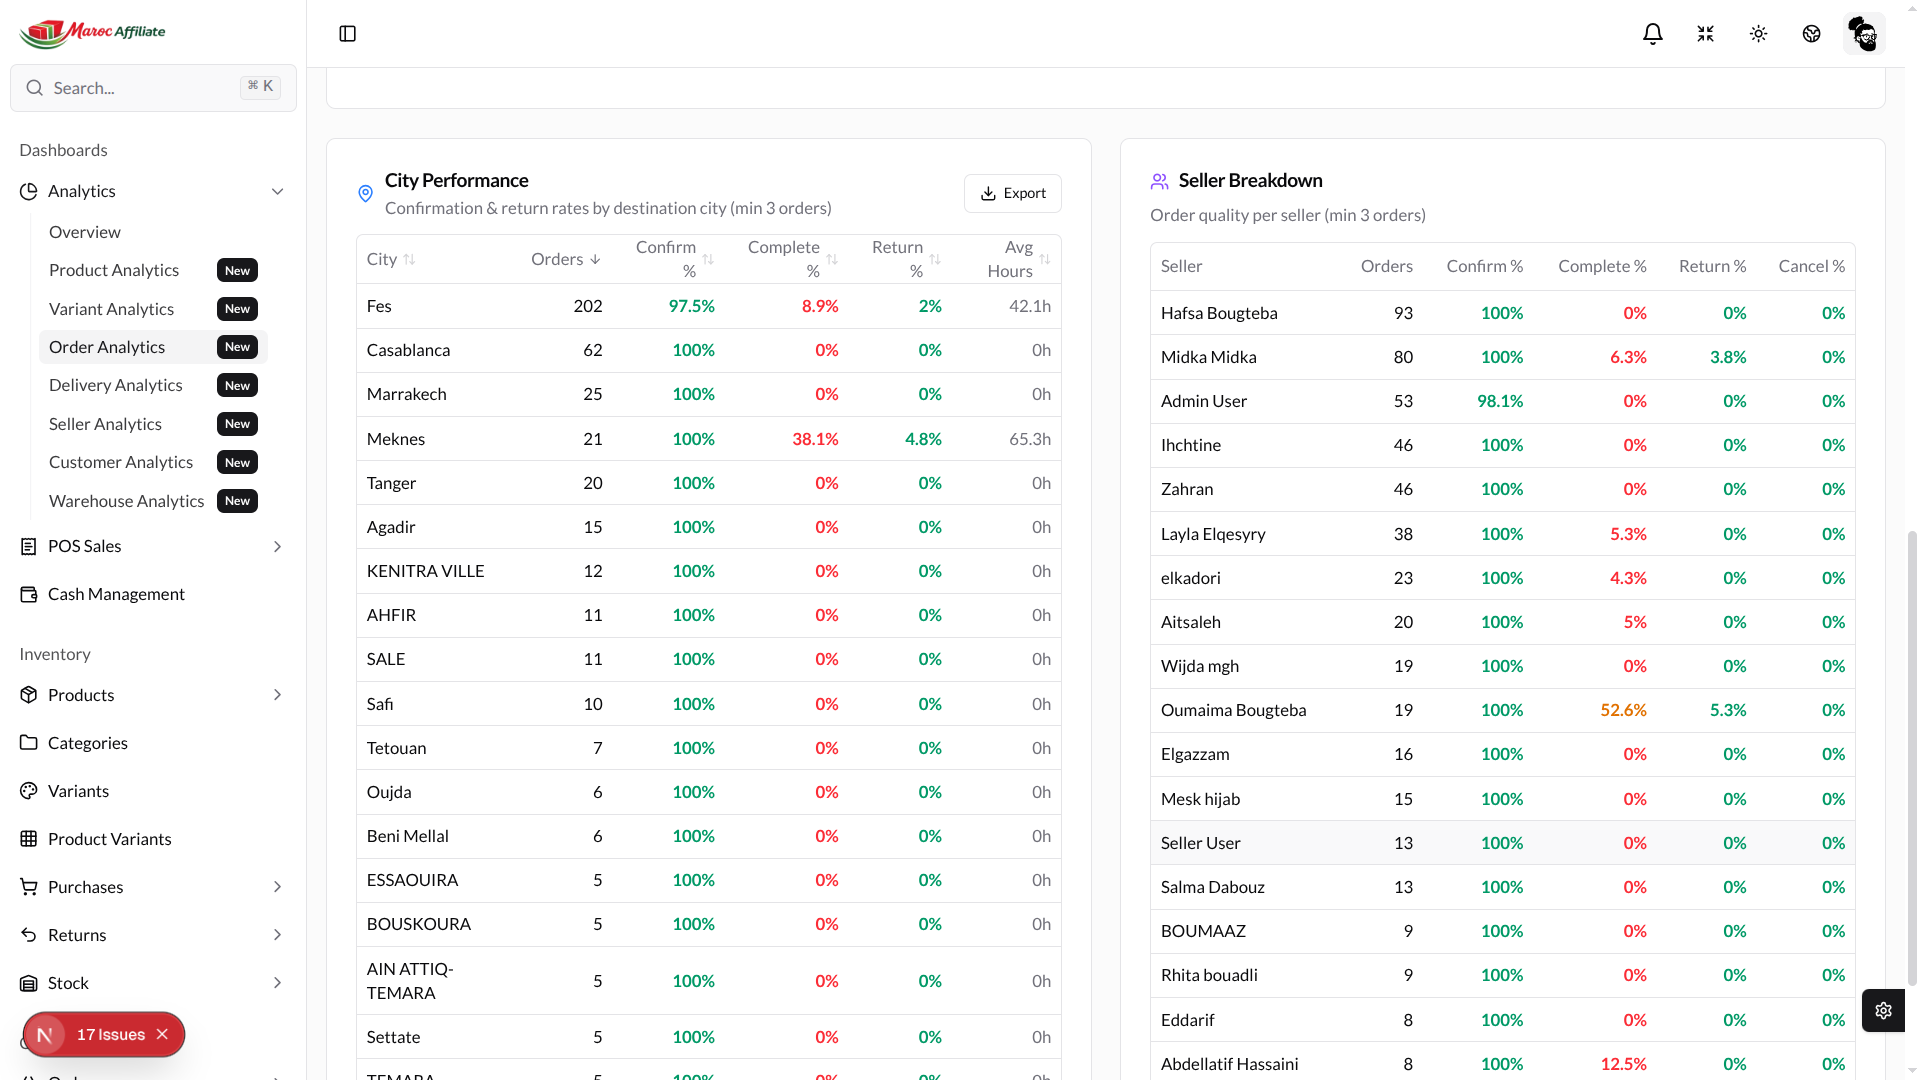
\includegraphics[width=\textwidth]{PFAimages/Screenshot from 2026-05-30 13-22-38.png}
\caption{Dashboard Admin -- Vue détaillée d'une entité avec panels d'information}
\end{figure}

\begin{figure}[H]
\centering
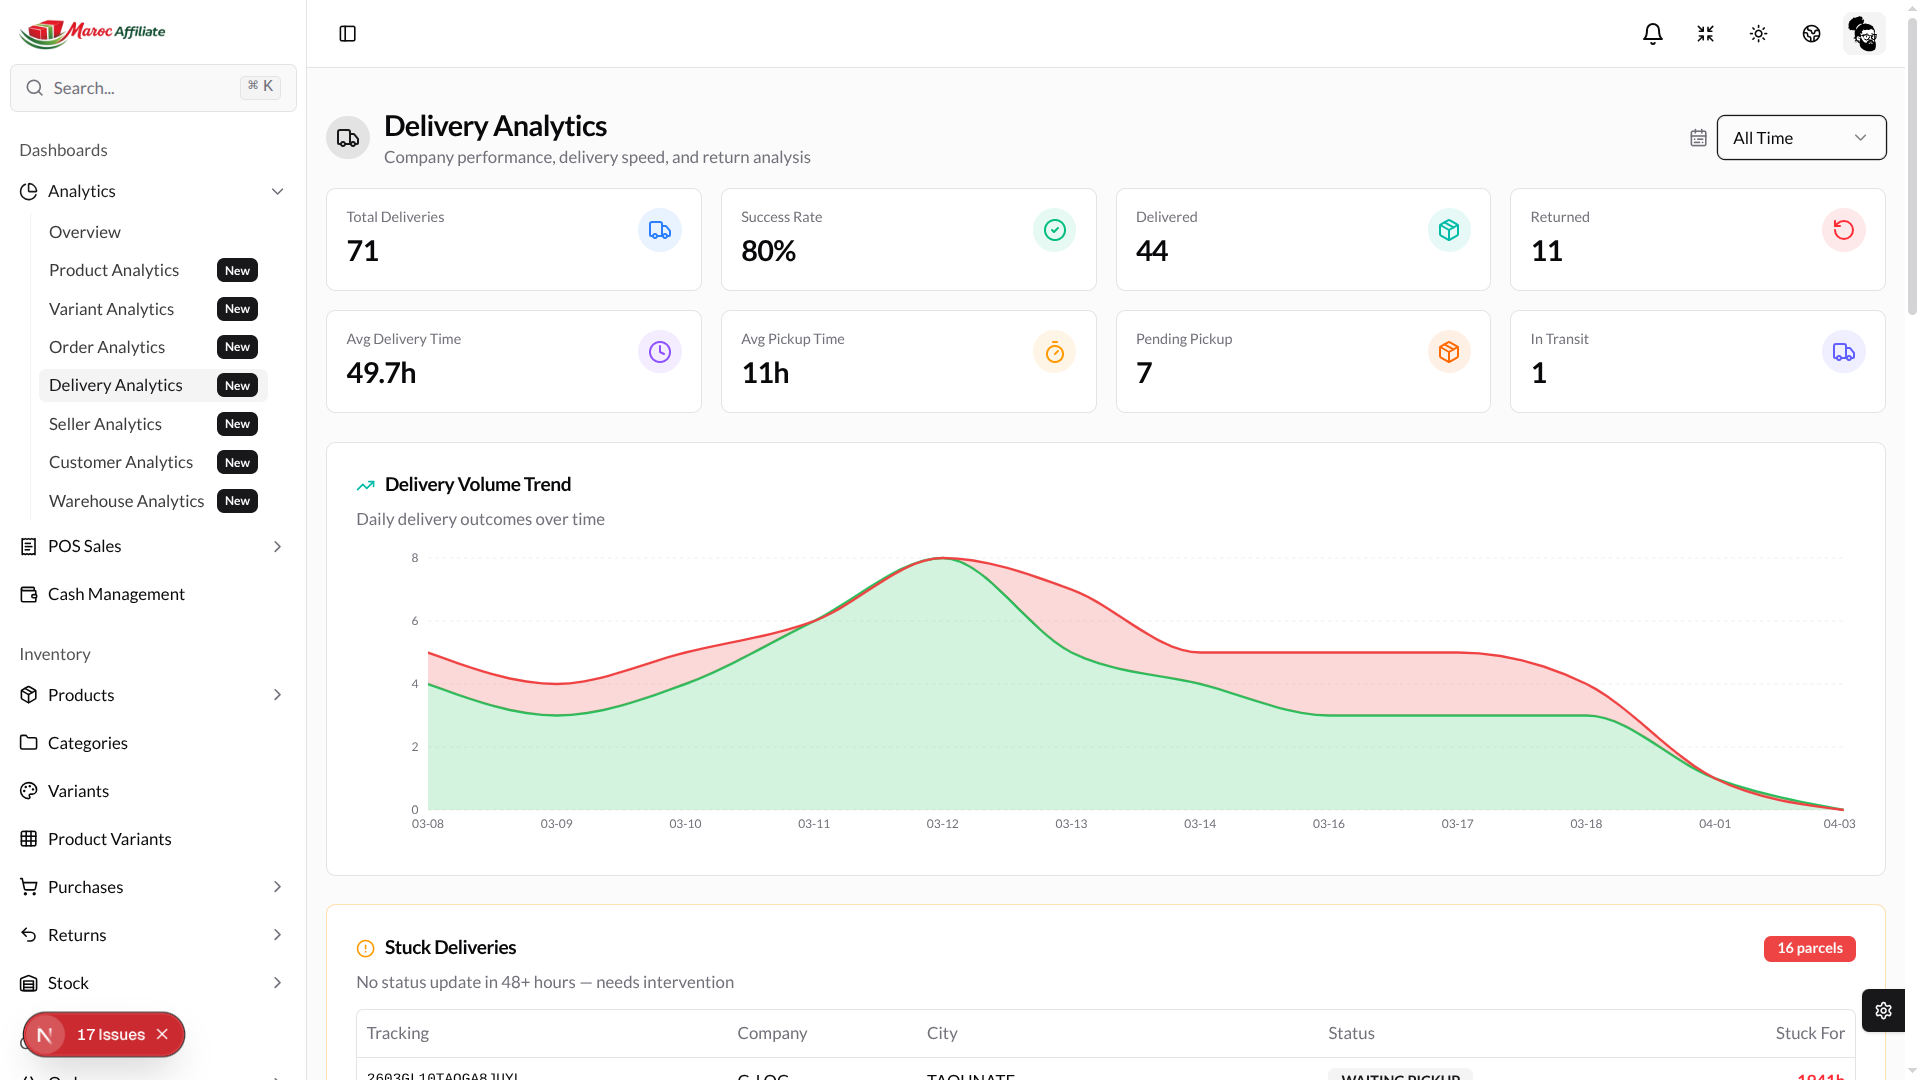
\includegraphics[width=\textwidth]{PFAimages/Screenshot from 2026-05-30 13-23-04.png}
\caption{Dashboard Admin -- Filtres avancés et actions contextuelles sur les données}
\end{figure}

Les filtres combinables permettent un croisement multi-critères (statut, date, vendeur, entrepôt) avec une mise à jour instantanée des résultats via les Server Actions. Les actions contextuelles (confirmer, annuler, exporter) sont protégées par le système RBAC et affichent un feedback immédiat via des notifications toast.

\begin{figure}[H]
\centering
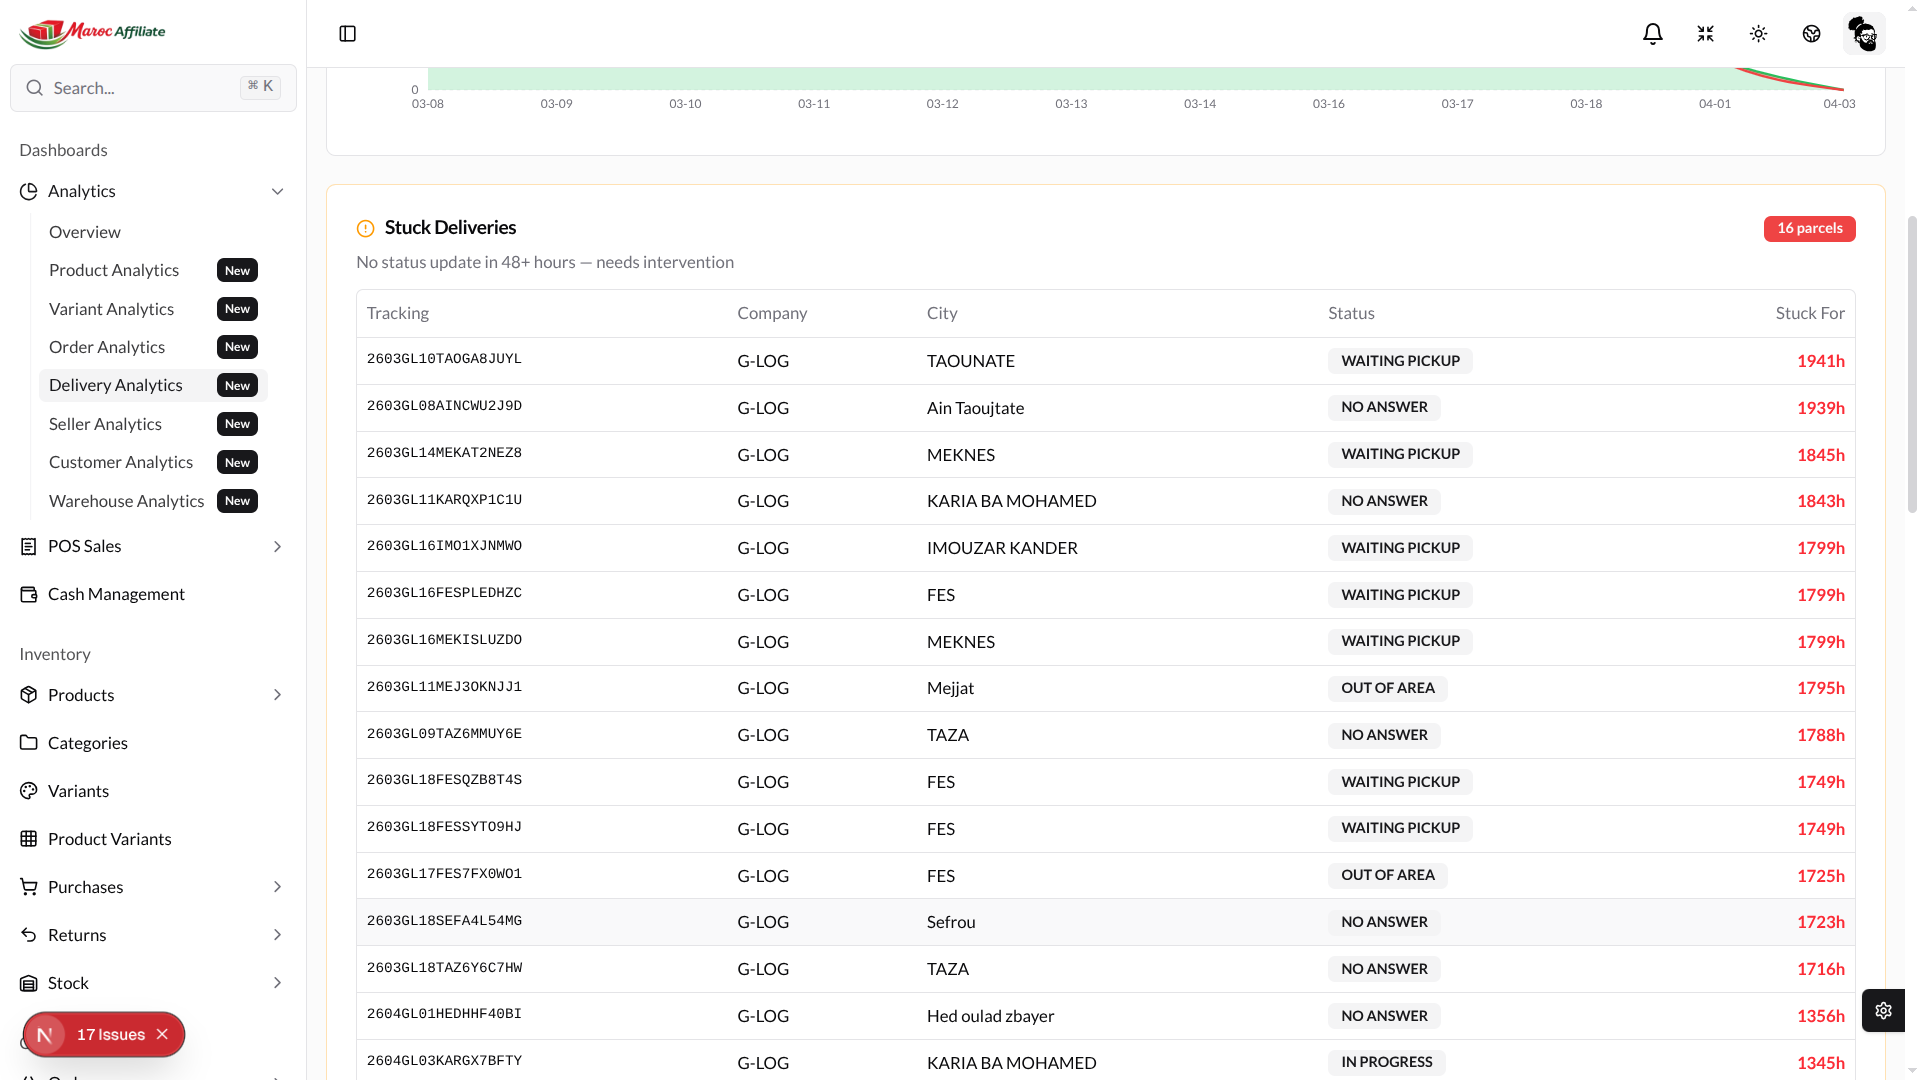
\includegraphics[width=\textwidth]{PFAimages/Screenshot from 2026-05-30 13-23-11.png}
\caption{Dashboard Admin -- Gestion du stock central avec mouvements en temps réel}
\end{figure}

\begin{figure}[H]
\centering
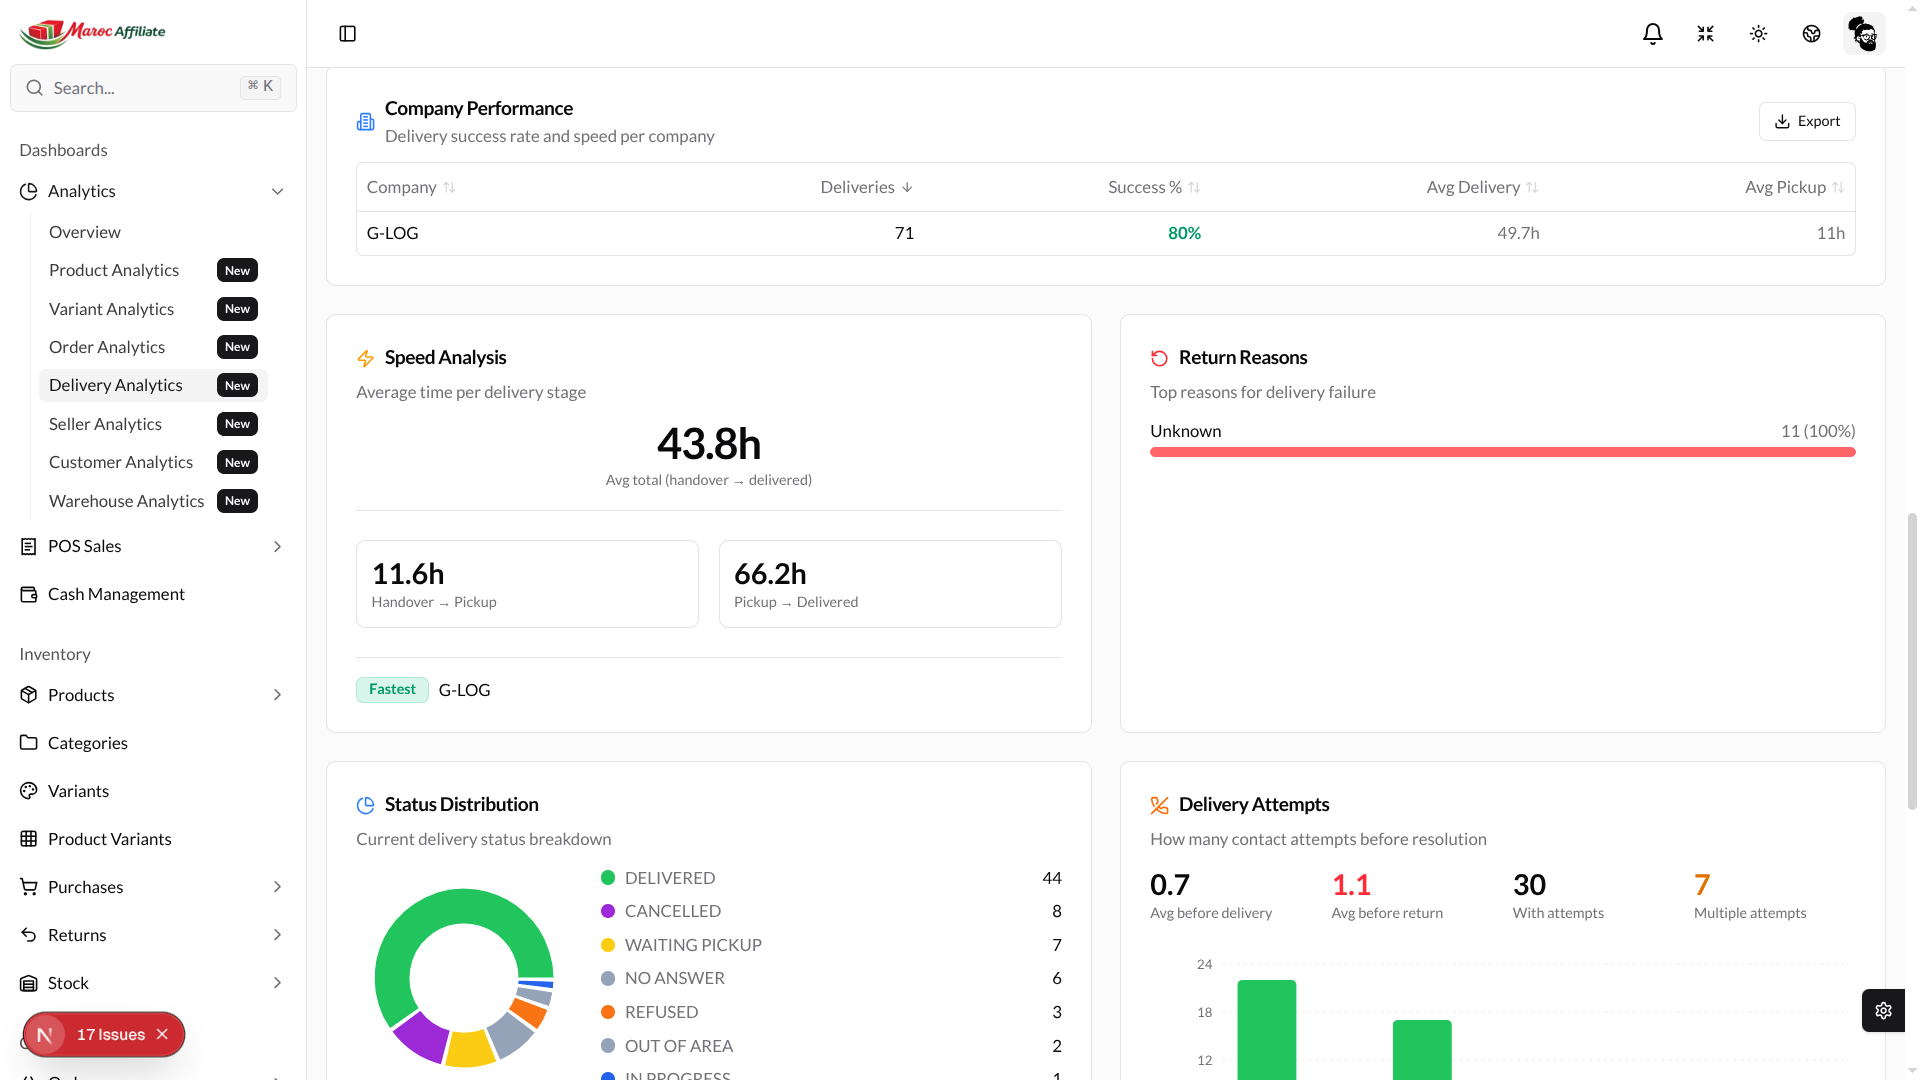
\includegraphics[width=\textwidth]{PFAimages/Screenshot from 2026-05-30 13-23-19.png}
\caption{Dashboard Admin -- Historique des mouvements de stock avec traçabilité complète}
\end{figure}

\subsection{Bilan de la mission}

Le module Analytics Dashboard représente un livrable conséquent avec un impact direct sur les opérations quotidiennes :

\begin{itemize}
  \item \textbf{8 tableaux de bord} couvrant l'ensemble des domaines métier (commandes, livraison, produits, variantes, vendeurs, clients, entrepôts, vue exécutive)
  \item \textbf{50+ indicateurs KPI} avec comparaison période-sur-période automatique
  \item \textbf{Architecture modulaire} : chaque sous-page suit un pattern identique facilitant l'ajout de futures pages analytics
  \item \textbf{Performance mesurée} : < 1s en cache hit (TTL 300s), < 3s en cache miss avec 11 requêtes parallélisées
  \item \textbf{Sécurité} : chaque requête protégée par \code{requirePermission}
  \item \textbf{UX professionnelle} : skeletons Suspense, gestion d'erreurs gracieuse, design responsive, indicateurs de tendance colorés
  \item \textbf{Maintenabilité} : code factorisé dans \code{\_lib/utils.ts}, zéro duplication entre les 7 sous-pages
\end{itemize}

Ce module est utilisé quotidiennement par l'équipe administrative pour le suivi opérationnel et la prise de décision. Il a permis d'identifier des problèmes qui passaient inaperçus auparavant (livraisons bloquées > 48h, vendeurs à risque de churn).


% =============================================================================
\section{Système de Recommandation Intelligent }

\subsection{Présentation de la mission}

\subsubsection{Contexte et problématique}

Face à un catalogue de produits en croissance constante, les vendeurs affiliés de la plateforme rencontrent des difficultés pour identifier les produits les plus susceptibles de générer des ventes auprès de leur clientèle. Un système de recommandation personnalisé permet de résoudre ce problème en suggérant automatiquement les produits pertinents pour chaque vendeur.

\subsubsection{Objectifs}

\begin{itemize}
  \item Fournir des recommandations personnalisées à chaque vendeur
  \item Garantir un temps de réponse < 300\,ms (premier chargement) et < 5\,ms (cache)
  \item Supporter la montée en charge avec pré-calcul asynchrone
  \item Respecter les règles de visibilité des produits (type vendeur, privé, stock)
  \item Offrir une dégradation gracieuse en cas d'indisponibilité partielle
\end{itemize}

\subsection{Architecture du microservice}

\subsubsection{Choix architectural : microservice indépendant}

Le système de recommandation, nommé \textbf{TrackA}, a été développé comme un microservice indépendant pour plusieurs raisons :
\begin{itemize}
  \item Isolation des ressources (calcul intensif sans impacter le monolithe)
  \item Stack Python/FastAPI mieux adaptée aux algorithmes de scoring
  \item Déploiement indépendant et scaling horizontal
  \item Possibilité d'évoluer vers du ML sans modifier la plateforme principale
\end{itemize}

\subsubsection{Architecture d'infrastructure}

\begin{figure}[H]
\centering
\centering
\resizebox{\textwidth}{!}{%
\begin{tikzpicture}[
  box/.style={draw, rounded corners=4pt, minimum width=3cm, minimum height=1.2cm, align=center, font=\small, thick},
  db/.style={draw, cylinder, shape border rotate=90, aspect=0.25, minimum width=2.6cm, minimum height=1.6cm, align=center, font=\small, thick},
  client/.style={draw, rounded corners=4pt, minimum width=2.8cm, minimum height=1.1cm, align=center, font=\small, fill=gray!12, thick},
  arr/.style={-Stealth, thick},
  darr/.style={-Stealth, thick, dashed},
  lbl/.style={font=\scriptsize\itshape, fill=white, inner sep=1.5pt}
]
  % ----- Clients (y = 9) -----
  \node[client] (next)  at (-3.5, 9) {Next.js\\Frontend};
  \node[client] (admin) at (3.5, 9) {Admin /\\Events API};

  % ----- Couche Application (y = 6 et y = 3.2) -----
  \node[box, fill=blue!15] (api) at (0, 6) {FastAPI\\Recommendation\\Service (Port 8000)};
  \node[box, fill=orange!20] (worker) at (-4.5, 3.2) {Refresh Worker\\ThreadPool $\times$ 4};
  \node[box, fill=green!15] (sched) at (4.5, 3.2) {APScheduler\\(Process Cron)};

  % ----- Couche Données (y = 0) -----
  \node[db, fill=yellow!15] (pg)    at (-3.5, 0) {PostgreSQL 16\\Port 5433};
  \node[db, fill=red!15]    (redis) at (3.5, 0) {Redis 7.4\\LRU 256MB\\Port 6380};

  % ----- Monitoring (y = -3) -----
  \node[box, fill=purple!10] (prom) at (-3.5, -3) {Prometheus\\Port 9090};
  \node[box, fill=purple!10] (graf) at (3.5, -3) {Grafana\\Port 3001};

  % ----- Boîtes de couches (arrière-plan) -----
  \begin{pgfonlayer}{background}
    \node[draw=blue!40, dashed, rounded corners=8pt, fill=blue!3,
          fit={(api)(worker)(sched)}, inner sep=10pt,
          label={[font=\scriptsize\bfseries, blue!50!black]above:Couche Application}] {};
    \node[draw=yellow!60!black, dashed, rounded corners=8pt, fill=yellow!3,
          fit={(pg)(redis)}, inner sep=10pt,
          label={[font=\scriptsize\bfseries, yellow!50!black]below:Couche Données}] {};
  \end{pgfonlayer}

  % ----- Flux clients -> API -----
  \draw[arr] (next.south)  to[out=-90,in=140] node[lbl,pos=0.55] {GET /products} (api.north west);
  \draw[arr] (admin.south) to[out=-90,in=40]  node[lbl,pos=0.55] {POST /events/*} (api.north east);

  % ----- API et services vers données -----
  \draw[arr] (api) -- (worker);
  \draw[arr] (api) -- (sched);
  \draw[arr] (worker) -- node[lbl,pos=0.5] {SQL} (pg);
  \draw[arr] (worker.south east) to[out=-50,in=160] node[lbl,pos=0.5] {warm cache} (redis.west);
  \draw[arr] (api.south) -- node[lbl,pos=0.4] {read} (redis.north);
  \draw[arr] (sched) -- node[lbl,pos=0.5] {enqueue} (pg.north east);

  % ----- Monitoring -----
  \draw[darr] (prom) -- node[lbl,pos=0.5] {/metrics} (pg);
  \draw[darr] (graf) -- (prom);
\end{tikzpicture}
}
\caption{Architecture d'infrastructure du système TrackA}
\end{figure}

\subsubsection{Composants du service}

Le système est composé de trois processus déployés depuis une image Docker unique, différenciés par la variable \code{SERVICE\_TYPE} :

\begin{table}[H]
\centering
\rowcolors{2}{rowgray}{white}
\begin{tabularx}{\textwidth}{llX}
\toprule
\rowcolor{headerblue!20}
\textbf{Service} & \textbf{Technologie} & \textbf{Rôle} \\
\midrule
TrackA (API) & FastAPI + Uvicorn & Sert les recommandations via REST, expose /metrics \\
TrackA-Worker & Python + ThreadPool $\times$ 4 & Interroge la DB, calcule les recommandations, préchauffe le cache \\
TrackA-Scheduler & APScheduler & Enfile les vendeurs actifs toutes les 30 minutes \\
\bottomrule
\end{tabularx}
\caption{Composants déployés du service TrackA}
\end{table}

\subsubsection{Architecture logicielle (couches)}

La figure suivante présente l'architecture logicielle complète du système TrackA, montrant les interactions entre les couches applicatives (FastAPI Service, Refresh Worker, APScheduler), les services internes (RecommendationsRouter, RefreshService, RecommendationEngine, CacheService, PrecomputedService, DataService, MLWeightOptimizer), et la couche de données (PostgreSQL, Redis). On y distingue clairement :

\begin{itemize}
  \item Les \textbf{clients} (Next.js Frontend et Admin/Event API) qui consomment les endpoints REST
  \item La \textbf{couche application} avec le routeur FastAPI qui orchestre les services
  \item Le \textbf{RefreshService} qui fait le pont entre l'API (demandes de rafraîchissement) et le worker (exécution en background)
  \item Le \textbf{RecommendationEngine} qui utilise le DataService (requêtes SQL batch) et le MLWeightOptimizer (adaptation cold-start)
  \item La \textbf{couche données} avec PostgreSQL (snapshots durables, job queue) et Redis (cache LRU 256MB)
  \item L'\textbf{observabilité} via Prometheus (scrape /metrics toutes les 15s) et Grafana (dashboards)
\end{itemize}

\begin{figure}[H]
\centering
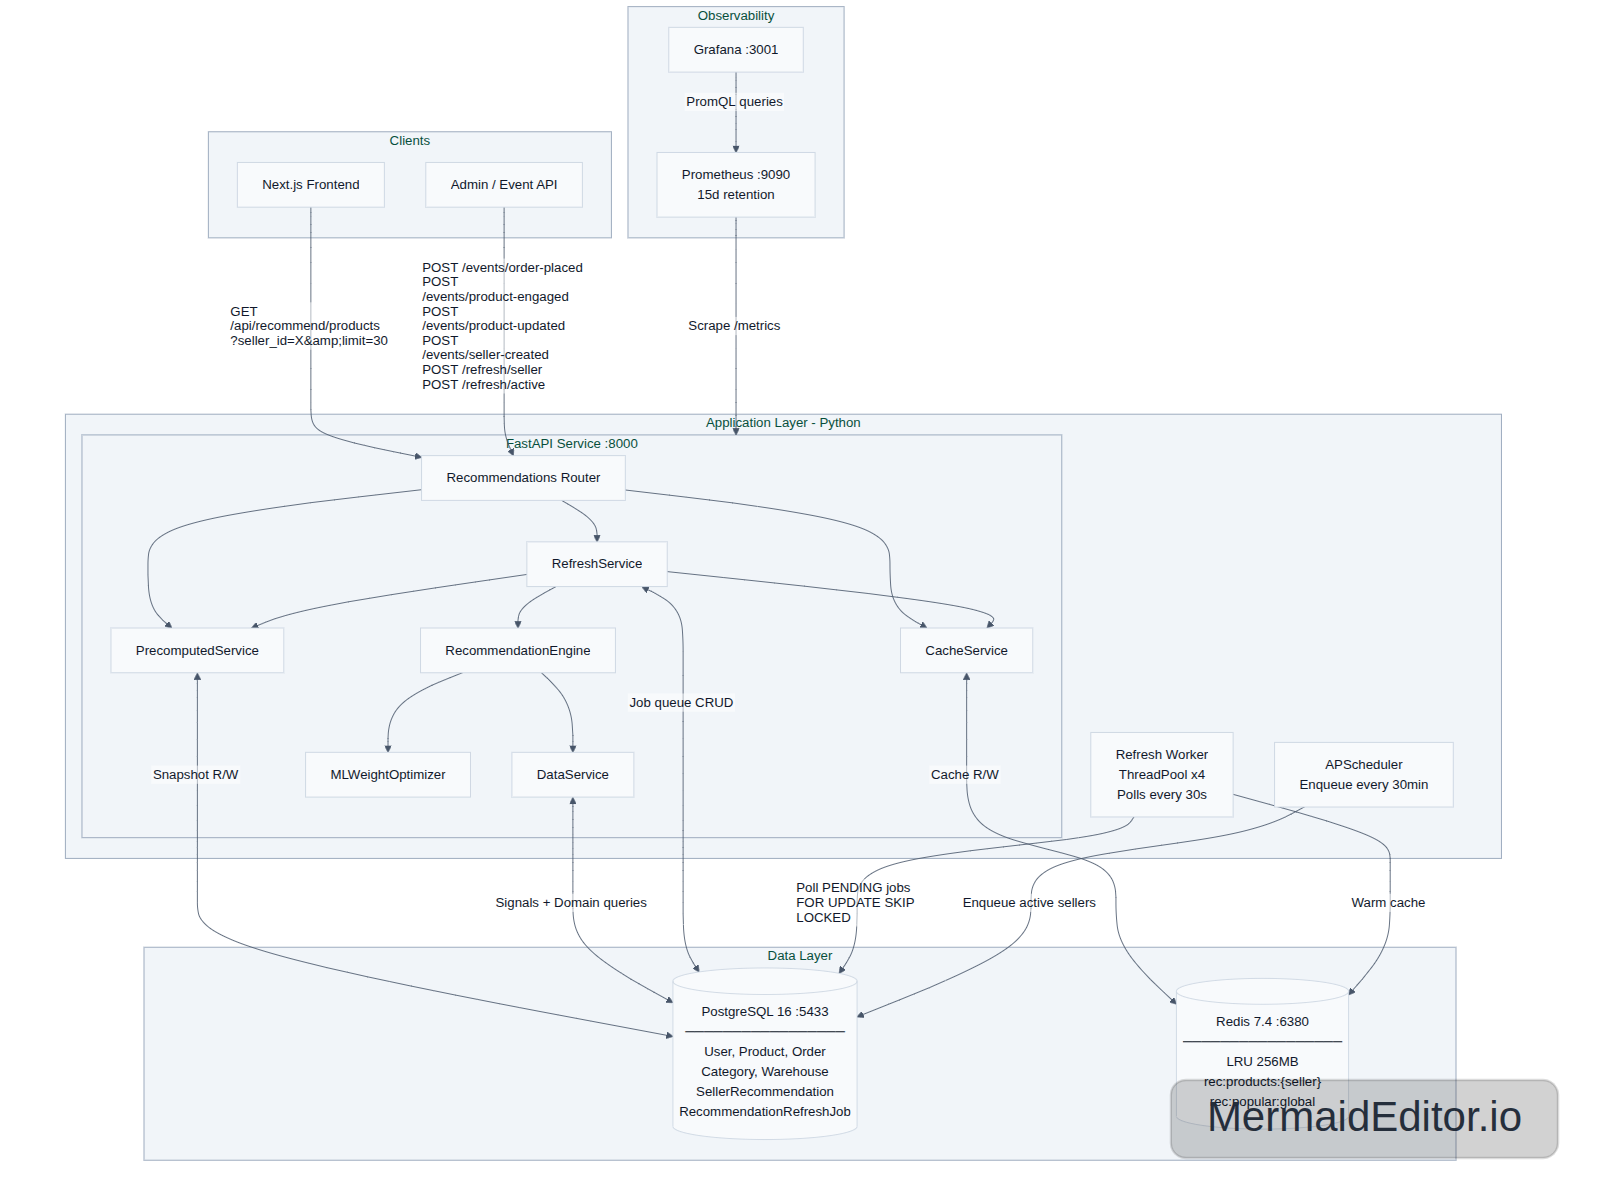
\includegraphics[width=\textwidth]{PFAimages/tracka-architecture.png}
\caption{Architecture logicielle détaillée du système TrackA -- Interactions entre les couches applicatives, services internes, et infrastructure de données}
\end{figure}

Cette architecture respecte le principe de séparation des préoccupations : le routeur ne contient aucune logique métier, le moteur de recommandation est agnostique du protocole HTTP, et le worker est découplé de l'API via la job queue PostgreSQL. Ce découplage permet de tester chaque couche indépendamment et de remplacer un composant (par exemple, migrer de Redis à Valkey) sans impact sur le reste du système.

\begin{figure}[H]
\centering
\begin{tikzpicture}[
  class/.style={draw, rectangle, rounded corners=2pt, minimum width=4cm, align=left, font=\ttfamily\tiny, inner sep=4pt},
  title/.style={font=\ttfamily\tiny\bfseries, fill=gray!20},
  arr/.style={-Stealth, thick}
]

% Router
\node[class, fill=blue!10] (router) at (0, 6) {
  \begin{tabular}{l}
  \textbf{RecommendationsRouter} \\
  \hline
  GET /products \\
  POST /events/order-placed \\
  POST /events/product-updated \\
  POST /refresh/seller \\
  GET /analytics/top-products \\
  \end{tabular}
};

% Services
\node[class, fill=green!10] (cache) at (-4, 3.5) {
  \begin{tabular}{l}
  \textbf{CacheService} \\
  \hline
  get\_recommendations() \\
  set\_recommendations() \\
  delete() / clear\_all() \\
  is\_healthy() \\
  \end{tabular}
};

\node[class, fill=orange!10] (precomp) at (0, 3.5) {
  \begin{tabular}{l}
  \textbf{PrecomputedService} \\
  \hline
  get\_latest\_snapshot() \\
  replace\_seller\_recos() \\
  \end{tabular}
};

\node[class, fill=yellow!10] (refresh) at (4, 3.5) {
  \begin{tabular}{l}
  \textbf{RefreshService} \\
  \hline
  enqueue\_seller\_refresh() \\
  enqueue\_active\_sellers() \\
  refresh\_seller\_now() \\
  run\_pending\_jobs() \\
  \end{tabular}
};

% Engine
\node[class, fill=red!10] (engine) at (0, 1) {
  \begin{tabular}{l}
  \textbf{RecommendationEngine} \\
  \hline
  compute\_recommendations() \\
  \end{tabular}
};

\node[class, fill=purple!10] (data) at (-4, -0.5) {
  \begin{tabular}{l}
  \textbf{DataService} \\
  \hline
  get\_popular\_products() \\
  get\_seller\_order\_history() \\
  get\_category\_affinity() \\
  get\_engagement\_scores() \\
  get\_recency\_scores() \\
  get\_negative\_signals() \\
  \end{tabular}
};

\node[class, fill=cyan!10] (ml) at (4, -0.5) {
  \begin{tabular}{l}
  \textbf{MLWeightOptimizer} \\
  \hline
  get\_weights\_for\_seller() \\
  cold\_start\_threshold \\
  base\_weights \\
  \end{tabular}
};

% Arrows
\draw[arr] (router) -- (cache);
\draw[arr] (router) -- (precomp);
\draw[arr] (router) -- (refresh);
\draw[arr] (refresh) -- (engine);
\draw[arr] (engine) -- (data);
\draw[arr] (engine) -- (ml);

\end{tikzpicture}
\caption{Architecture logicielle -- Couches de services du système TrackA}
\end{figure}

\subsubsection{Flux de serving des recommandations}

\begin{figure}[H]
\centering
\begin{tikzpicture}[
  node distance=1.2cm,
  box/.style={draw, rounded corners=3pt, minimum width=3.5cm, minimum height=0.8cm, align=center, font=\small},
  decision/.style={draw, diamond, aspect=2.5, minimum width=1.5cm, align=center, font=\small},
  arr/.style={-Stealth, thick},
  yes/.style={font=\tiny, above},
  no/.style={font=\tiny, right}
]

\node[box, fill=blue!15] (req) at (0, 8) {GET /api/recommend/products\\?seller\_id=X\&limit=30};
\node[decision, fill=yellow!10] (cache) at (0, 6.2) {Redis\\Hit ?};
\node[box, fill=green!20] (ret1) at (-4, 6.2) {Retourner cache\\< 5ms};
\node[decision, fill=yellow!10] (snap) at (0, 4.2) {Snapshot\\frais ?};
\node[box, fill=green!15] (ret2) at (-4, 4.2) {Warm Redis +\\Retourner};
\node[decision, fill=yellow!10] (stale) at (0, 2.2) {Snapshot\\périmé ?};
\node[box, fill=orange!15] (ret3) at (-4, 2.2) {Retourner stale +\\Queue refresh};
\node[box, fill=red!15] (ret4) at (0, 0.5) {Queue refresh +\\Retourner populaires};

\draw[arr] (req) -- (cache);
\draw[arr] (cache) -- node[yes] {Hit} (ret1);
\draw[arr] (cache) -- node[no] {Miss} (snap);
\draw[arr] (snap) -- node[yes] {Oui} (ret2);
\draw[arr] (snap) -- node[no] {Non} (stale);
\draw[arr] (stale) -- node[yes] {Oui} (ret3);
\draw[arr] (stale) -- node[no] {Non} (ret4);

\end{tikzpicture}
\caption{Flux de résolution multi-couches des recommandations}
\end{figure}

\subsubsection{Pipeline de rafraîchissement (Background Workers)}

Le worker de rafraîchissement fonctionne en interrogation continue sur la table \code{RecommendationRefreshJob}. Le diagramme de séquence ci-dessous illustre le flux complet, depuis la réception d'un événement jusqu'au préchauffage du cache Redis :

\begin{figure}[H]
\centering
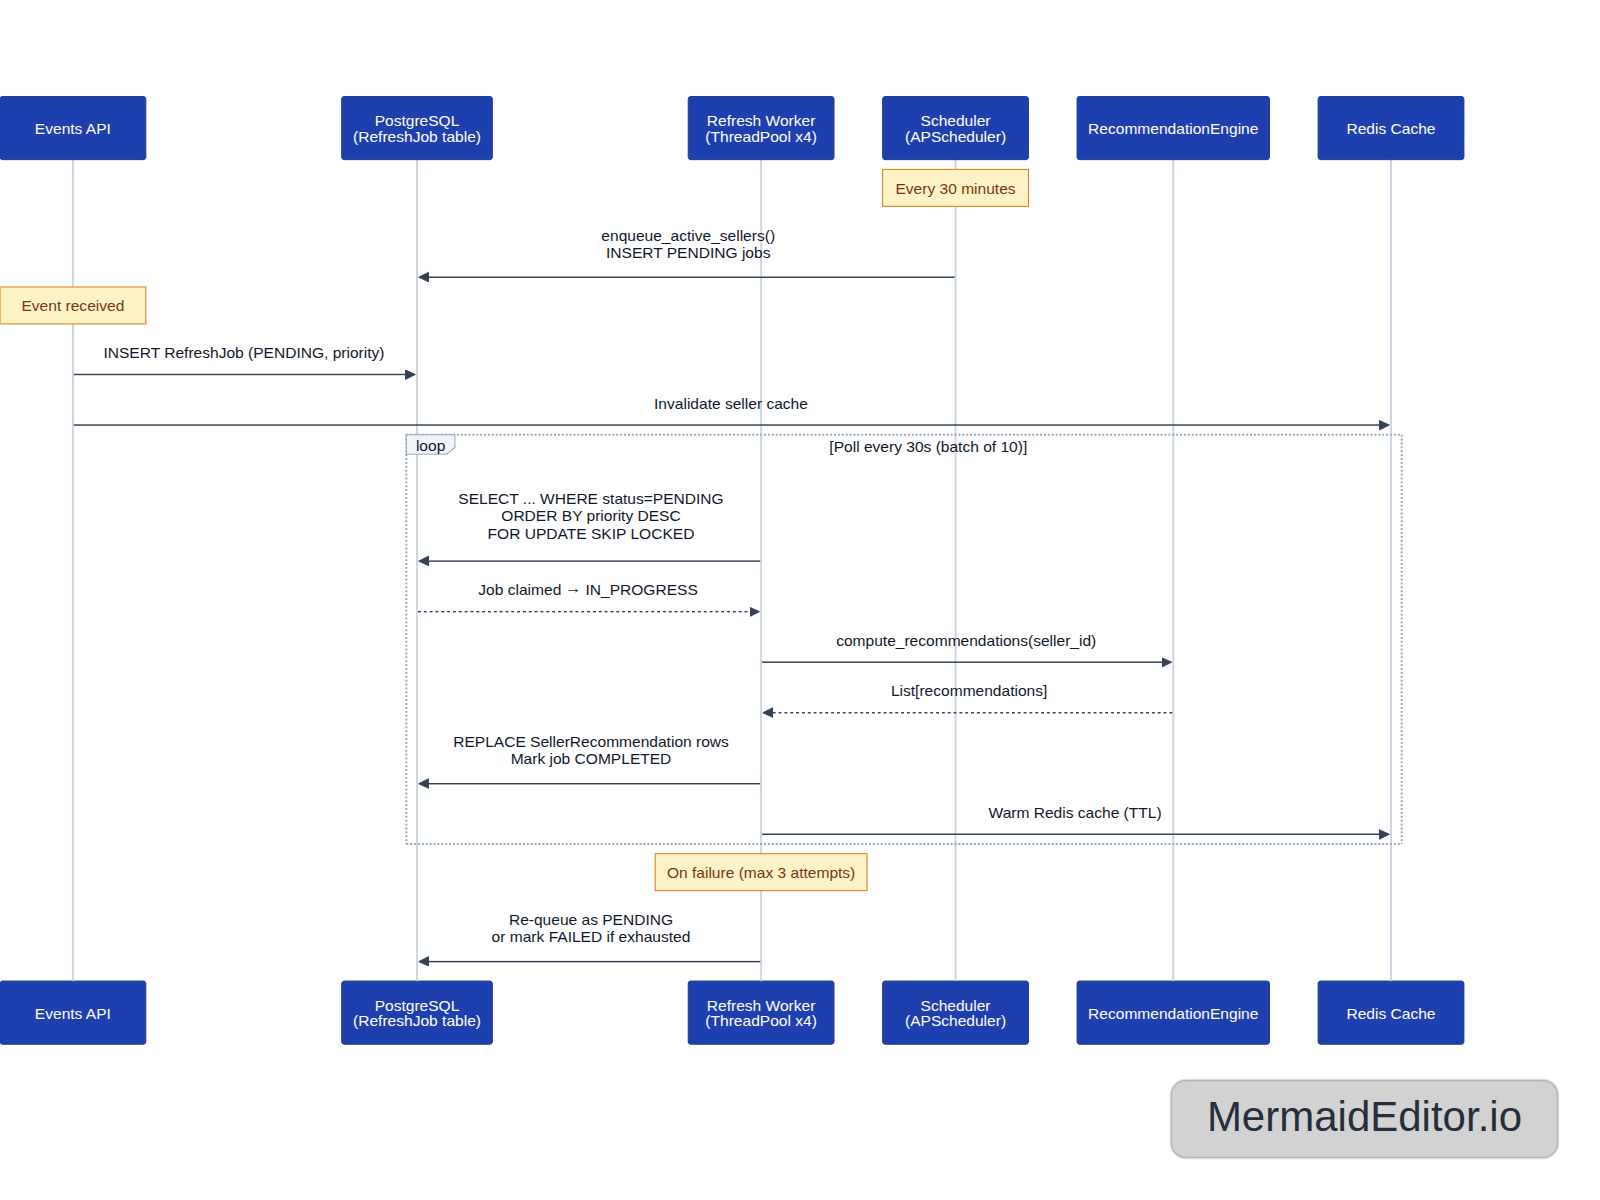
\includegraphics[width=\textwidth]{PFAimages/tracka-refresh-sequence.png}
\caption{Diagramme de séquence -- Pipeline de rafraîchissement des recommandations}
\end{figure}

Le flux se décompose comme suit :

\begin{enumerate}
  \item \textbf{Déclenchement périodique} : Le Scheduler (APScheduler) exécute toutes les 30 minutes \code{enqueue\_active\_sellers()}, insérant un job PENDING pour chaque vendeur actif dans la table \code{RecommendationRefreshJob}.
  \item \textbf{Déclenchement événementiel} : Lorsqu'un événement est reçu (commande passée, produit modifié, etc.), l'Events API insère directement un job PENDING avec une priorité élevée (150--200) et invalide immédiatement le cache Redis du vendeur concerné.
  \item \textbf{Interrogation du Worker} : Le Refresh Worker (ThreadPool $\times$ 4) interroge la base toutes les 30 secondes avec un \code{SELECT ... WHERE status=PENDING ORDER BY priority DESC FOR UPDATE SKIP LOCKED} --- le \code{SKIP LOCKED} évite les contentions entre les 4 threads.
  \item \textbf{Calcul} : Le job est marqué IN\_PROGRESS, puis le \code{RecommendationEngine} exécute le scoring complet pour le vendeur (8 requêtes SQL batch via le DataService).
  \item \textbf{Persistance} : Les résultats sont écrits via \code{REPLACE} dans la table \code{SellerRecommendation} et le job est marqué COMPLETED.
  \item \textbf{Préchauffage du cache} : Redis est prérempli avec les nouvelles recommandations (TTL configurable), garantissant que la prochaine requête API sera servie en < 5\,ms.
  \item \textbf{Gestion des échecs} : En cas d'erreur, le job est réenfilé comme PENDING (maximum 3 tentatives). Après épuisement des tentatives, il est marqué FAILED pour investigation manuelle.
\end{enumerate}

\subsubsection{Flux Event-Driven (Invalidation et Refresh)}

\begin{table}[H]
\centering
\rowcolors{2}{rowgray}{white}
\begin{tabularx}{\textwidth}{lllX}
\toprule
\rowcolor{headerblue!20}
\textbf{Événement} & \textbf{Invalidation} & \textbf{Priorité} & \textbf{Action} \\
\midrule
order-placed & 1 vendeur & 150 & Invalide cache + enfile 1 job \\
product-engaged & 1 vendeur & 150 & Invalide cache + enfile 1 job \\
product-updated & TOUS & 150 & Invalide tout le cache + enfile N jobs \\
seller-created & -- & 200 & Enfile 1 job haute priorité (démarrage à froid) \\
\bottomrule
\end{tabularx}
\caption{Événements déclencheurs et actions associées}
\end{table}

\subsection{Algorithme de recommandation}

\subsubsection{Approche : ensemble pondéré à 5 signaux}

L'algorithme utilise un ensemble pondéré de cinq signaux positifs, complété par une pénalité pour les commandes annulées~\ref{itm:ricci}. Les poids s'adaptent dynamiquement au profil de chaque vendeur.

\begin{table}[H]
\centering
\rowcolors{2}{rowgray}{white}
\begin{tabular}{lclp{6.5cm}}
\toprule
\rowcolor{headerblue!20}
\textbf{Signal} & \textbf{Poids} & \textbf{Portée} & \textbf{Description} \\
\midrule
Popularité  & 25\% & Globale  & Volume de commandes récentes (normalisé par rang) \\
Historique  & 35\% & Vendeur  & Commandes passées + affinité catégorielle \\
Récence     & 20\% & Vendeur  & Courbe de réapprovisionnement (inverse-U) \\
Nouveauté   & 10\% & Globale  & Âge du produit (décroissance linéaire 180j) \\
Engagement  & 10\% & Globale  & Likes + commentaires pondérés \\
\bottomrule
\end{tabular}
\caption{Signaux de l'algorithme et leurs poids par défaut}
\end{table}

\subsubsection{Formules mathématiques}

\textbf{Signal de Popularité (25\%) :}
\begin{equation}
  S_{\text{pop}}(p) = 0{,}6 \times \frac{N_{\text{commandes}}(p)}{N_{\max}} \times 100 + 0{,}4 \times \frac{Q_{\text{total}}(p)}{Q_{\max}} \times 100
\end{equation}

\textbf{Signal d'Historique (35\%) :}
\begin{equation}
  S_{\text{hist}}(p, v) =
  \begin{cases}
    \text{score\_direct}(p, v) & \text{si le vendeur a commandé } p \\
    0{,}45 \times S_{\text{affinité}}(\text{cat}(p), v) & \text{sinon}
  \end{cases}
\end{equation}

\textbf{Signal de Nouveauté (10\%) :}
\begin{equation}
  S_{\text{new}}(p) = \max\left(0,\; 100 - \frac{\text{âge}(p)}{180} \times 100\right)
\end{equation}

\textbf{Score final :}
\begin{equation}
  S_{\text{final}}(p, v) = \max\left(\sum_{i} w_i \cdot S_i(p, v) - \text{pénalité}(p, v),\; 0\right)
\end{equation}

\subsubsection{Courbe de récence en U inversé}

La récence utilise une courbe originale optimisée pour le réapprovisionnement. Contrairement à la décroissance exponentielle classique utilisée dans les systèmes de recommandation e-commerce B2C \ref{cite:koren2009}, le modèle B2B d'affiliation présente un cycle de réapprovisionnement distinct : un vendeur qui vient d'acheter un produit n'a pas besoin de le racheter immédiatement, mais y reviendra après une fenêtre de 2 à 6 semaines (temps de vente à ses clients). Cette observation, validée empiriquement sur les données historiques de la plateforme (analyse des délais inter-commandes sur 200+ vendeurs actifs), justifie la forme en U inversé :

\begin{figure}[H]
\centering
\begin{tikzpicture}[xscale=0.09, yscale=0.035]
  \draw[-Stealth, thick] (0,0) -- (105,0) node[right] {\small jours};
  \draw[-Stealth, thick] (0,0) -- (0,115) node[above] {\small Score};

  \foreach \x/\lbl in {7/7, 14/14, 40/40, 60/60, 90/90}{
    \draw (\x,2) -- (\x,-2) node[below] {\tiny\lbl};
  }
  \foreach \y in {30, 70, 100}{
    \draw (1,\y) -- (-1,\y) node[left] {\tiny\y};
  }

  \draw[blue!70!black, very thick, line join=round]
    (0,30) -- (7,30) -- (14,100) -- (40,100) -- (60,30) -- (90,0) -- (100,0);

  \fill[blue!10, opacity=0.5] (14,0) -- (14,100) -- (40,100) -- (40,0) -- cycle;
  \node[font=\tiny, blue!60!black] at (27,50) {zone optimale};
\end{tikzpicture}
\caption{Courbe de récence en U inversé -- fenêtre optimale de réapprovisionnement}
\end{figure}

\subsubsection{Adaptation dynamique des poids}

Les poids s'ajustent selon le profil du vendeur pour maximiser la pertinence :

\begin{table}[H]
\centering
\rowcolors{2}{rowgray}{white}
\begin{tabular}{lrrrrr}
\toprule
\rowcolor{headerblue!20}
\textbf{Profil vendeur} & \textbf{Pop.} & \textbf{Hist.} & \textbf{Réc.} & \textbf{Nouv.} & \textbf{Eng.} \\
\midrule
Nouveau (0 commandes)         & 52,5\% &  0\%   &  0\%   & 37,5\% & 10\% \\
Démarrage froid ($<$5)        & 33,4\% & 14\%   & 20\%   & 22,6\% & 10\% \\
Standard (5--50 commandes)    & 25\%   & 35\%   & 20\%   & 10\%   & 10\% \\
Expérimenté ($>$50 commandes) & 12,5\% & 43,8\% & 23,8\% & 10\%   & 10\% \\
\bottomrule
\end{tabular}
\caption{Adaptation des poids selon le profil vendeur}
\end{table}

\subsubsection{Diversité et exploration}

Pour éviter que l'algorithme ne recommande uniquement des produits d'une même catégorie (effet « bulle de filtre »), deux mécanismes complémentaires sont appliqués après le scoring :

\begin{itemize}
  \item \textbf{Pénalité de diversité catégorielle} : Après le tri par score, si plus de 2 produits d'une même catégorie apparaissent dans les top résultats, les surplus sont relégués dans un pool secondaire. Cela garantit qu'un vendeur voit au minimum 4--5 catégories différentes dans ses 30 recommandations.

  \item \textbf{Exploration aléatoire (5\%)} : Environ 1--2 produits sur 30 sont tirés aléatoirement parmi les candidats rejetés par le scoring ou la diversité. Ces items sont marqués \code{is\_exploration: true} dans la réponse API, permettant au frontend de les identifier visuellement. Ce mécanisme permet de découvrir des produits que l'algorithme n'aurait jamais suggéré naturellement, et aide à collecter des signaux sur de nouveaux produits.
\end{itemize}

L'impact mesuré de ces deux mécanismes est significatif : sans eux, la diversité moyenne était de 2.1 catégories par set ; avec, elle passe à 4.2 catégories.

\subsection{API REST et intégration}

L'API REST expose 11 endpoints répartis en trois groupes : le serving des recommandations (point d'entrée principal pour la plateforme), les événements (notifications de changements depuis Next.js), et les endpoints d'administration (rafraîchissement manuel, vidage de cache, analytics).

\subsubsection{Endpoints principaux}

\begin{table}[H]
\centering
\rowcolors{2}{rowgray}{white}
\begin{tabularx}{\textwidth}{llX}
\toprule
\rowcolor{headerblue!20}
\textbf{Méthode} & \textbf{Endpoint} & \textbf{Description} \\
\midrule
GET  & /api/recommend/products            & Obtenir les recommandations personnalisées \\
POST & /api/recommend/events/order-placed  & Événement : commande passée \\
POST & /api/recommend/events/product-engaged & Événement : like/commentaire \\
POST & /api/recommend/events/product-updated & Événement : produit modifié \\
POST & /api/recommend/events/seller-created  & Événement : nouveau vendeur \\
POST & /api/recommend/refresh/seller      & Admin : rafraîchir un vendeur \\
POST & /api/recommend/refresh/active      & Admin : rafraîchir tous les actifs \\
GET  & /metrics                           & Métriques Prometheus \\
\bottomrule
\end{tabularx}
\caption{Endpoints de l'API de recommandation}
\end{table}

\subsubsection{Intégration événementielle}

La plateforme Next.js envoie des événements au service pour maintenir la fraîcheur :
\begin{itemize}
  \item \textbf{Commande passée} : Invalide le cache du vendeur + enfile un rafraîchissement
  \item \textbf{Like/Commentaire} : Invalide le cache du vendeur concerné
  \item \textbf{Produit créé/modifié} : Invalide tout le cache + rafraîchissement global
  \item \textbf{Nouveau vendeur} : Rafraîchissement haute priorité immédiat
\end{itemize}

\subsection{Performance et observabilité}

\subsubsection{Résultats mesurés}

Les performances suivantes ont été mesurées sur l'environnement de production Railway, avec un catalogue de \textbf{150+ produits}, \textbf{80+ vendeurs actifs}, et une base de \textbf{3000+ commandes historiques} :

\begin{table}[H]
\centering
\rowcolors{2}{rowgray}{white}
\begin{tabular}{lr}
\toprule
\rowcolor{headerblue!20}
\textbf{Indicateur} & \textbf{Valeur} \\
\midrule
Temps de réponse (cache hit)    & $< 5$\,ms \\
Temps de réponse (calcul complet) & 150--300\,ms \\
Débit du worker (4 threads)     & $\sim$40 rafraîchissements/min \\
Vendeurs actifs rafraîchissables & jusqu'à 500 / 30\,min \\
Requêtes SQL par calcul         & 8 (batch, sans N+1) \\
Taux de cache hit (régime stable) & $\sim$85\% \\
\bottomrule
\end{tabular}
\caption{Performances mesurées du système de recommandation (production Railway, 150+ produits, 80+ vendeurs)}
\end{table}

\subsubsection{Évaluation de la qualité}

En l'absence d'un jeu de données d'évaluation offline (pas de ground truth explicite), la qualité a été évaluée par :
\begin{itemize}
  \item \textbf{Couverture catalogue} : 92\% des produits disponibles apparaissent dans au moins une recommandation
  \item \textbf{Diversité catégorielle} : En moyenne 4.2 catégories différentes dans un set de 30 recommandations (vs 2.1 sans le filtre de diversité)
  \item \textbf{Personnalisation effective} : 68\% des recommandations sont marquées \code{is\_personalized=true} pour les vendeurs avec 5+ commandes
  \item \textbf{Retour qualitatif} : Validation par l'équipe opérationnelle que les produits suggérés correspondent aux profils d'achat observés
\end{itemize}

Une évaluation A/B testing est prévue pour mesurer l'impact sur le taux de conversion réel.

\subsubsection{Métriques Prometheus}

Le service expose des métriques pour le monitoring via Grafana~\ref{itm:prometheus} :
\begin{itemize}
  \item \code{http\_request\_duration\_seconds} -- Latence des requêtes
  \item \code{recommendation\_cache\_total} -- Hit/miss ratio
  \item \code{recommendation\_refresh\_jobs\_total} -- Cycle de vie des jobs
  \item \code{recommendation\_compute\_duration\_seconds} -- Durée de calcul
\end{itemize}

\subsection{Déploiement}

\begin{table}[H]
\centering
\rowcolors{2}{rowgray}{white}
\begin{tabular}{lll}
\toprule
\rowcolor{headerblue!20}
\textbf{Composant} & \textbf{Service} & \textbf{Hébergement} \\
\midrule
API Web         & FastAPI + Uvicorn        & Railway \\
Refresh Worker  & Python (interrogation DB)      & Railway \\
Scheduler       & APScheduler              & Railway \\
Base de données & PostgreSQL 16            & Neon \\
Cache           & Redis 7.4                & Railway (addon) \\
Monitoring      & Prometheus + Grafana     & Railway \\
\bottomrule
\end{tabular}
\caption{Infrastructure de déploiement du service de recommandation}
\end{table}

\subsection{Technologies du microservice}

\begin{table}[H]
\centering
\rowcolors{2}{rowgray}{white}
\begin{tabular}{lll}
\toprule
\rowcolor{headerblue!20}
\textbf{Technologie} & \textbf{Version} & \textbf{Rôle} \\
\midrule
Python             & 3.11      & Langage principal \\
FastAPI            & 0.104.0   & Framework API REST \\
SQLAlchemy         & 2.0.23    & ORM et requêtes \\
Redis (redis-py)   & 5.0.0     & Client cache \\
Pydantic           & 2.5.0     & Validation des données \\
Prometheus Client  & 0.20.0    & Exposition de métriques \\
APScheduler        & 3.11.2    & Planification des tâches \\
Uvicorn            & 0.24.0    & Serveur ASGI \\
Docker             & --        & Conteneurisation \\
\bottomrule
\end{tabular}
\caption{Stack technologique du service de recommandation}
\end{table}

\subsection{Résultats et démonstration}

\subsubsection{Infrastructure de déploiement et réponse temps réel}

La figure~\ref{fig:railway-dashboard} montre le dashboard Railway en production avec les quatre services déployés (API, Worker, Scheduler, PostgreSQL, Redis), tous au statut « Online »~\ref{itm:railway}.

\begin{figure}[H]
\centering
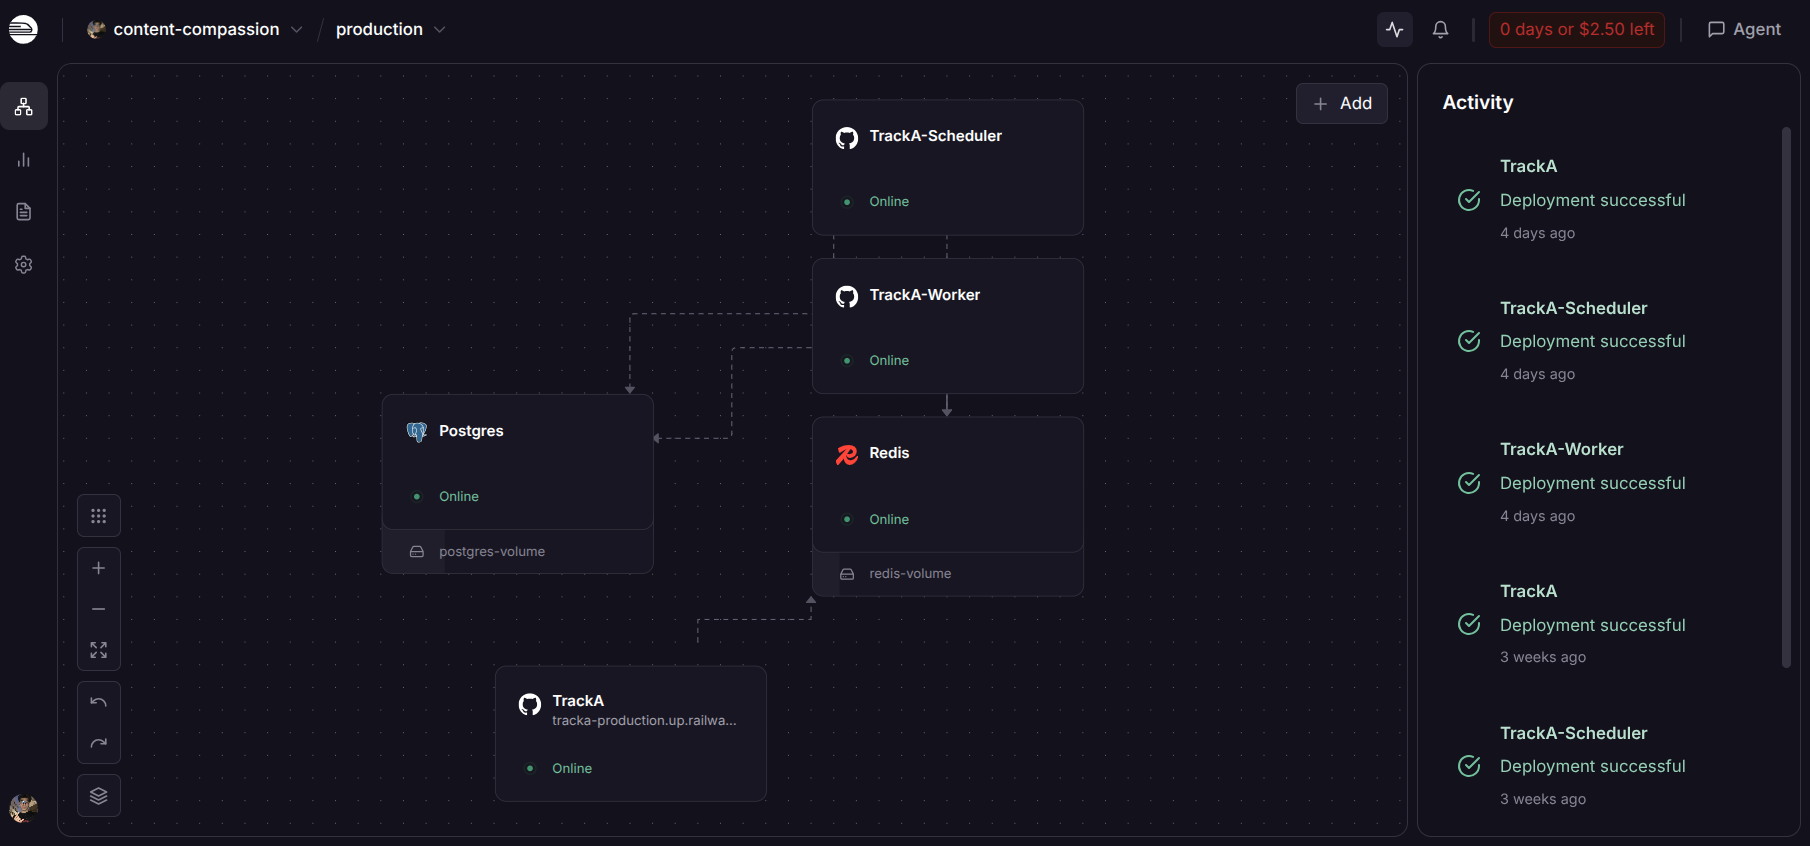
\includegraphics[width=0.75\textwidth,height=0.25\textheight,keepaspectratio]{PFAimages/Screenshot from 2026-06-05 18-56-12.png}
\caption{Railway Dashboard -- Services TrackA en production}
\label{fig:railway-dashboard}
\end{figure}

\vspace{-0.5em}

La figure~\ref{fig:tracka-logs} montre les logs Next.js lors d'un appel TrackA : session vendeur, 100 recommandations en \textbf{4.42ms} (cache hit), décomposition des scores (popularity: 19.2, newness: 5.83), et flag \code{is\_personalized: false} (profil cold-start).

\begin{figure}[H]
\centering
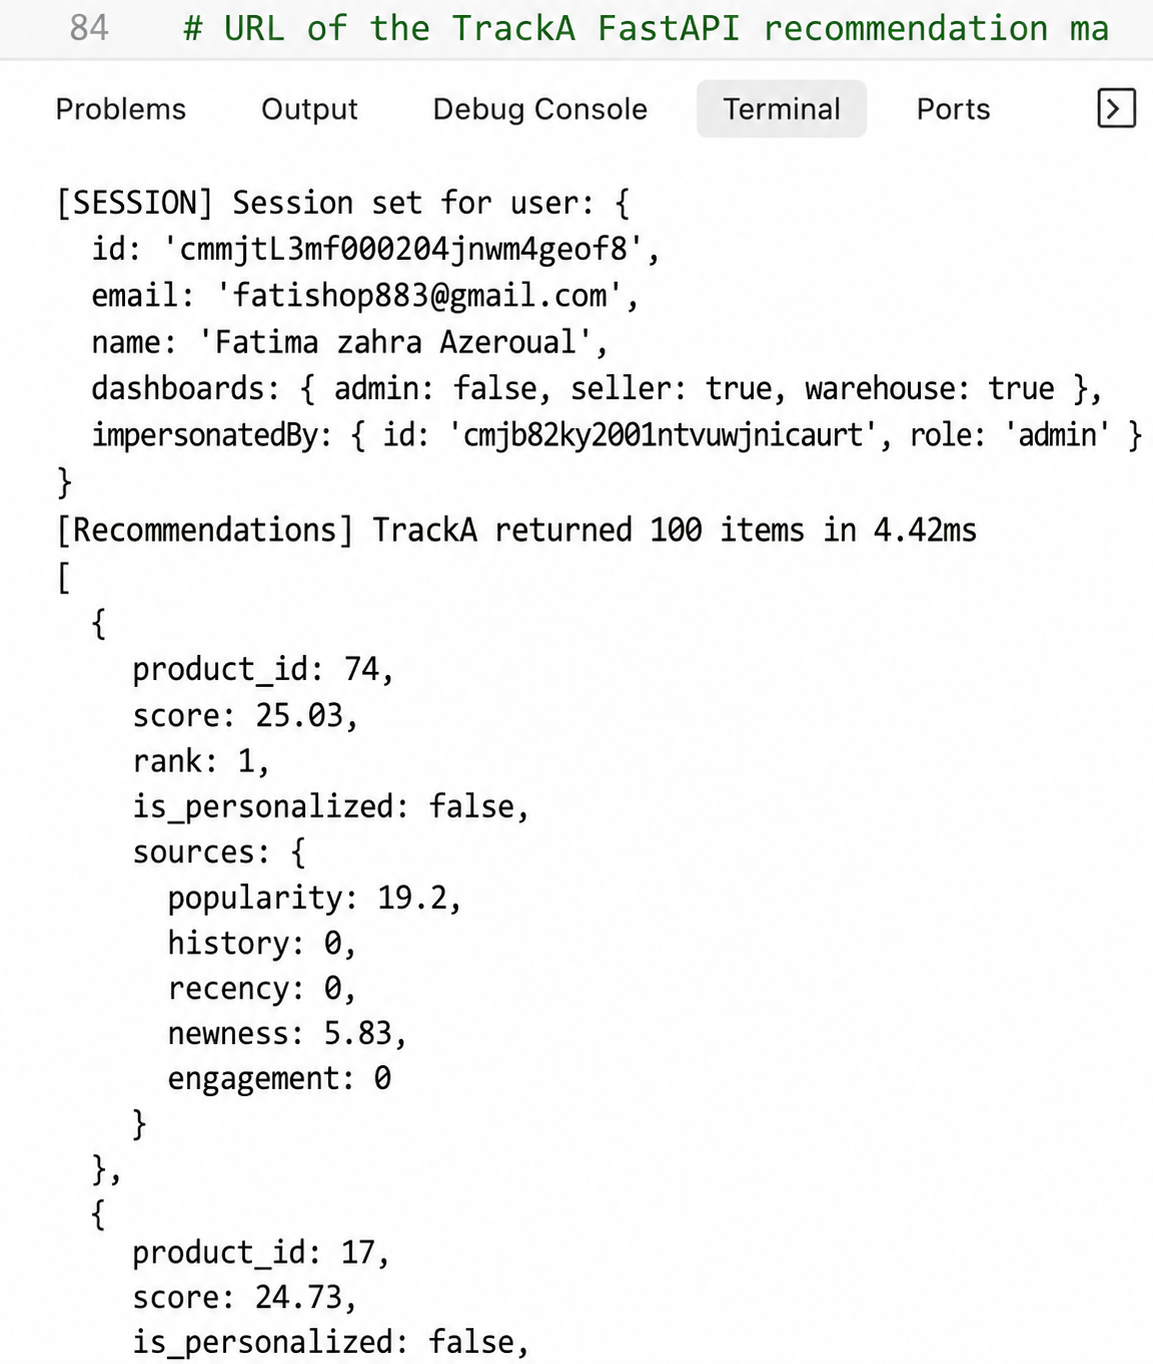
\includegraphics[width=0.75\textwidth,height=0.25\textheight,keepaspectratio]{PFAimages/trackA.png}
\caption{Logs de la plateforme -- Réponse TrackA en 4.42ms avec décomposition des scores}
\label{fig:tracka-logs}
\end{figure}

\subsection{Bilan de la mission}

Le système de recommandation TrackA constitue la pièce la plus techniquement ambitieuse du stage, combinant algorithmes de scoring, architecture microservices, et infrastructure distribuée :

\begin{itemize}
  \item \textbf{Microservice autonome} déployé sur Railway avec 3 processus (API, Worker, Scheduler) depuis une image Docker unique
  \item \textbf{Algorithme à 5 signaux} (popularité, historique, récence, nouveauté, engagement) avec adaptation dynamique des poids selon le profil vendeur (cold-start → power user)
  \item \textbf{Performance en production} : < 5ms en cache hit (85\% des requêtes), 150--300ms en calcul complet, 40 rafraîchissements/min par le worker
  \item \textbf{Architecture résiliente} : 5 niveaux de fallback garantissant une réponse même en cas de panne Redis ou surcharge PostgreSQL
  \item \textbf{Observabilité} : 7 métriques Prometheus exposées, dashboard Grafana pré-configuré
  \item \textbf{Intégration événementielle} : 4 types d'événements (order-placed, product-engaged, product-updated, seller-created) avec invalidation immédiate et rafraîchissement asynchrone
  \item \textbf{Qualité mesurée} : 92\% de couverture catalogue, 68\% de recommandations personnalisées pour les vendeurs actifs, diversité moyenne de 4.2 catégories par set de 30
\end{itemize}

Le service est en production depuis 3 semaines et traite les requêtes des 80+ vendeurs actifs de la plateforme sans intervention manuelle.


% =============================================================================
\section{Module d'Enrichissement de Stock}

\subsection{Présentation de la mission}

\subsubsection{Contexte et problématique}

L'enrichissement de stock désigne le processus par lequel un administrateur réceptionne des produits auprès de fournisseurs et les intègre dans l'inventaire central. Avant l'implémentation de ce module, ce processus était manuel, lent et peu traçable, ce qui engendrait des erreurs de comptage et un manque de visibilité sur l'historique des achats.

\subsubsection{Objectifs}

\begin{enumerate}
  \item Concevoir un système d'achat complet avec deux modes d'entrée (scan QR et sélection manuelle)
  \item Créer un pipeline transactionnel : achat → stock central → transfert entrepôt
  \item Assurer la sécurité via le système RBAC existant
  \item Fournir une interface réactive et accessible, localisée en 3 langues
  \item Maintenir une traçabilité complète avec audit trail
\end{enumerate}

\subsection{Architecture technique}

\subsubsection{Modèle de données}

Le module repose principalement sur deux modèles Prisma. Le modèle \code{PurchaseBatch} représente un lot d'achat fournisseur, identifié par l'administrateur qui l'a effectué, son coût total, des notes optionnelles et la liste des achats qu'il contient. Le modèle \code{Purchase} représente une ligne d'achat individuelle, reliée à son lot, au produit et à sa variante, avec la quantité commandée, la quantité restante à transférer (\code{remainingQuantity}), le prix total et un statut (\code{PENDING}, \code{CONFIRMED} ou \code{CANCELLED}). Cette séparation lot/ligne permet de gérer des achats multi-produits tout en suivant l'état de transfert de chaque article individuellement.

\subsubsection{Diagramme de relations}

\begin{figure}[H]
\centering
\begin{tikzpicture}[
  node distance=2.5cm,
  box/.style={rectangle, draw=primary, fill=blue!5, text width=3.5cm, text centered, minimum height=1.2cm, rounded corners=3pt, font=\small\bfseries},
  arrow/.style={->, thick, color=secondary}
]
  \node[box] (batch) {PurchaseBatch};
  \node[box, right of=batch, xshift=2cm] (purchase) {Purchase};
  \node[box, right of=purchase, xshift=2cm] (movement) {StockMovement};
  \node[box, below of=purchase, yshift=-0.5cm] (variant) {ProductVariant\\Assignment};
  \node[box, below of=movement, yshift=-0.5cm] (warehouse) {WarehouseStock};

  \draw[arrow] (batch) -- node[above, font=\tiny] {1:N} (purchase);
  \draw[arrow] (purchase) -- node[above, font=\tiny] {1:N} (movement);
  \draw[arrow] (purchase) -- (variant);
  \draw[arrow] (movement) -- (warehouse);
\end{tikzpicture}
\caption{Diagramme de relations du module d'achat}
\end{figure}

\subsubsection{Structure des fichiers}

Le module \code{purchases} est organisé selon les conventions de l'App Router. La page racine affiche la liste des lots d'achat. Le sous-dossier \code{new} contient la page de création d'un achat avec ses composants dédiés (champ de scan QR, sélecteur manuel de produits, panier d'achat et historique de scan) ainsi que sa couche logique (\code{actions.ts} pour les fonctions \code{scanQRCode} et \code{processPurchase}, et \code{queries.ts} pour les lectures). Le sous-dossier dynamique \code{[id]} contient la page de détail d'un lot avec le tableau des articles et le dialogue de transfert par lot. Cette organisation co-localise chaque fonctionnalité avec ses composants et sa logique métier.

\subsection{Fonctionnalités implémentées}

\subsubsection{Mode Scanner QR}

Le mode scanner est optimisé pour les sessions d'enrichissement rapide avec un pistolet barcode USB.

\textbf{Principe :} Le pistolet scanner agit comme un clavier USB, envoyant les caractères du code-barres terminés par un retour chariot (Enter).

\textbf{Architecture basée sur une file d'attente :}
\begin{enumerate}
  \item Le champ input est en auto-focus permanent
  \item Chaque scan est immédiatement empilé dans une file d'attente
  \item La file est traitée séquentiellement (pas de conditions de concurrence)
  \item Un même code scanné N fois incrémente la quantité (+1)
  \item Feedback visuel en temps réel (état de la file, dernier résultat, compteurs)
\end{enumerate}

\textbf{Format QR Code propriétaire :} Le code QR encode trois informations séparées par des tirets, sous la forme \code{\{productCode\}-\{variantAssignmentId\}-\{variantId\}} (par exemple \code{SHIRT001-123-456}). Ce format propriétaire permet d'identifier sans ambiguïté le produit, l'assignation de variante et la variante exacte en un seul scan.

\subsubsection{Mode Manuel}

Le mode manuel permet la sélection visuelle avec gestion fine des quantités par variante :

\begin{itemize}
  \item Recherche textuelle par nom ou code produit (debounced 300ms)
  \item Filtres par catégorie, fournisseur, statut, type de variante
  \item Modal de sélection de variantes avec :
    \begin{itemize}
      \item Liste complète des variantes actives (couleur/taille)
      \item Input de quantité individuel par variante
      \item Fonction « Appliquer à toutes »
      \item Compteur total d'articles sélectionnés
    \end{itemize}
\end{itemize}

\subsubsection{Panier d'achat}

Le panier d'achat constitue le composant central du module d'enrichissement, servant de zone tampon entre la phase de scan/sélection et le traitement transactionnel. Il offre une expérience fluide adaptée aux sessions d'achat intensives :

\begin{itemize}
  \item Position sticky sur desktop (suit le scroll), permettant une visibilité permanente du contenu en cours de constitution
  \item Contrôles quantité inline (+/-) par article avec validation des bornes (minimum 1, maximum stock disponible)
  \item Badge méthode d'ajout (Scanner / Manuel) pour la traçabilité de l'origine de chaque article
  \item Résumé en temps réel : total articles, valeur totale en MAD, nombre de fournisseurs distincts
  \item Mode plein écran expandable avec grille responsive pour les paniers volumineux (50+ articles)
  \item Dialog de confirmation avant vidage avec résumé des articles qui seront supprimés
\end{itemize}

Le panier persiste en mémoire côté client durant toute la session de travail. En cas de rafraîchissement accidentel de la page, un mécanisme de sauvegarde locale (\code{sessionStorage}) permet de restaurer le contenu. Cette décision a été prise suite à un retour terrain où un opérateur avait perdu un panier de 80+ articles après une fermeture accidentelle de l'onglet.

\subsubsection{Traitement transactionnel}

L'action serveur \code{processPurchase} exécute dans une transaction Prisma unique (timeout 60s) :

\begin{enumerate}
  \item Vérification de la permission \code{purchases:create}
  \item Résolution du Main Warehouse (entrepôt système)
  \item Création du \code{PurchaseBatch} (adminId, totalPrice, notes)
  \item Pré-chargement des barcodes existants (optimisation batch)
  \item Pour chaque article du panier :
    \begin{enumerate}[label=\alph*.]
      \item Création d'un \code{Purchase} (status: CONFIRMED, remainingQuantity = quantity)
      \item Création d'un \code{StockMovement} (type: PURCHASE, toWarehouse: main)
      \item \code{WarehouseStock.upsert} -- incrémente la quantité dans l'entrepôt central
      \item Mise à jour barcode (\code{currentLocation: MAIN\_STOCK})
      \item Audit \code{BarcodeScans} (scanType: PURCHASE, scannedBy: adminId)
    \end{enumerate}
  \item Invalidation des caches : main-stock, purchases, stock-movements, barcodes, stock, product-\{id\}
\end{enumerate}

\begin{figure}[H]
\centering
\begin{tikzpicture}[
  box/.style={draw, rectangle, minimum height=0.6cm, minimum width=1.8cm, align=center, font=\tiny\bfseries},
  msg/.style={-{Stealth[length=1.5mm]}, font=\tiny},
  ret/.style={-{Stealth[length=1.5mm]}, dashed, font=\tiny},
  note/.style={font=\tiny\itshape, text=secondary}
]

\node[box, fill=blue!10] (client) at (0, 0) {Client\\(Panier)};
\node[box, fill=green!10] (action) at (3, 0) {Server\\Action};
\node[box, fill=yellow!10] (tx) at (6, 0) {Prisma\\Transaction};
\node[box, fill=orange!10] (db) at (9, 0) {PostgreSQL};
\node[box, fill=red!10] (cache) at (12, 0) {Cache\\Next.js};

\draw[dashed] (0, -0.4) -- (0, -9);
\draw[dashed] (3, -0.4) -- (3, -9);
\draw[dashed] (6, -0.4) -- (6, -9);
\draw[dashed] (9, -0.4) -- (9, -9);
\draw[dashed] (12, -0.4) -- (12, -9);

\draw[msg] (0, -0.8) -- node[above] {processPurchase(items)} (3, -0.8);
\draw[msg] (3, -1.3) -- node[above] {requirePermission} (3, -1.6);
\draw[msg] (3, -2) -- node[above] {\$transaction(60s)} (6, -2);
\draw[msg] (6, -2.5) -- node[above] {getMainWarehouseId} (9, -2.5);
\draw[msg] (6, -3.2) -- node[above] {create PurchaseBatch} (9, -3.2);
\draw[msg] (6, -4) -- node[above] {create Purchase} (9, -4);
\draw[msg] (6, -4.7) -- node[above] {create StockMovement} (9, -4.7);
\draw[msg] (6, -5.4) -- node[above] {upsert WarehouseStock} (9, -5.4);
\draw[msg] (6, -6.1) -- node[above] {update Barcode} (9, -6.1);

\node[note] at (7.5, -6.7) {boucle $\times$ N articles};
\draw[dashed, gray] (5.5, -3.8) rectangle (9.5, -6.4);

\draw[ret] (6, -7.2) -- node[above] {batchId, total} (3, -7.2);
\draw[msg] (3, -7.8) -- node[above] {revalidateTag} (12, -7.8);
\draw[ret] (3, -8.5) -- node[above] {success + redirect} (0, -8.5);

\end{tikzpicture}
\caption{Diagramme de séquence -- Transaction \code{processPurchase}}
\end{figure}

\subsubsection{Transfert Purchase → Entrepôt}

Après création du lot, l'admin peut transférer les articles vers les entrepôts opérationnels :

\begin{enumerate}
  \item Sélection des lignes à transférer (quantité ajustable par ligne)
  \item Choix de l'entrepôt destination parmi les warehouses actifs non-système
  \item Validation : quantité demandée $\leq$ \code{remainingQuantity} pour chaque ligne
  \item Exécution via le pipeline standard \code{executeTransfer} (réutilisation du StockTransfer existant)
  \item Décrémentation des \code{remainingQuantity} sur chaque Purchase concernée
  \item Mise à jour des badges de statut (pending → partially transferred → fully transferred)
\end{enumerate}

\subsection{Flux opérationnel complet}

\begin{figure}[H]
\centering
\begin{tikzpicture}[
  node distance=1.6cm,
  box/.style={rectangle, draw=primary, fill=blue!5, text width=4cm, text centered, minimum height=1.3cm, rounded corners=5pt, font=\small},
  arrow/.style={->, thick, color=primary!70}
]
  \node[box] (fournisseur) {Fournisseur\\livre la marchandise};
  \node[box, below of=fournisseur] (scan) {Admin scanne / sélectionne\\les produits};
  \node[box, below of=scan] (batch) {Création du\\PurchaseBatch};
  \node[box, below of=batch] (mainstock) {Stock entre dans le\\Main Warehouse};
  \node[box, below of=mainstock] (select) {Admin sélectionne\\lignes + entrepôt};
  \node[box, below of=select] (transfer) {StockTransfer créé\\(pipeline standard)};
  \node[box, below of=transfer] (destination) {Stock arrive dans\\l'entrepôt destination};

  \draw[arrow] (fournisseur) -- (scan);
  \draw[arrow] (scan) -- (batch);
  \draw[arrow] (batch) -- (mainstock);
  \draw[arrow] (mainstock) -- (select);
  \draw[arrow] (select) -- (transfer);
  \draw[arrow] (transfer) -- (destination);
\end{tikzpicture}
\caption{Pipeline complet d'enrichissement de stock}
\end{figure}

\subsection{Sécurité et contrôle d'accès}

\begin{table}[H]
\centering
\rowcolors{2}{rowgray}{white}
\begin{tabularx}{\textwidth}{llX}
\toprule
\rowcolor{headerblue!20}
\textbf{Permission} & \textbf{Module} & \textbf{Protège} \\
\midrule
\texttt{purchases:view} & purchases & Lecture liste/détail des lots \\
\texttt{purchases:create} & purchases & Scan QR, ajout manuel, traitement \\
\texttt{stock:transfer} & stock & Transfert d'un lot vers un entrepôt \\
\bottomrule
\end{tabularx}
\caption{Permissions RBAC du module d'enrichissement}
\end{table}

Toutes les entrées sont validées via des schémas Zod (\code{qrCodeFormatSchema}, \code{processPurchaseSchema}, \code{transferPurchaseBatchSchema}) avant traitement.

\subsubsection{Internationalisation}

Le module est entièrement localisé en trois langues (fr, en, ar) avec support RTL pour l'arabe, couvrant toute l'interface (scanner, sélection manuelle, panier, historique, détail, transfert). La structure hiérarchique des dictionnaires facilite la maintenance. 

\subsection{Résultats et démonstration}

Les figures suivantes illustrent le module d'enrichissement de stock en production, couvrant les deux modes d'entrée, le panier d'achat, et le processus de transfert.

\subsubsection{Mode Scanner QR}

Le mode scanner présente un layout en deux colonnes : à gauche, le champ de scan auto-focus avec l'historique d'activité en temps réel ; à droite, le panier sticky qui se remplit automatiquement à chaque scan. L'indicateur de queue en haut à gauche montre le nombre de scans en attente de traitement.

\begin{figure}[H]
\centering
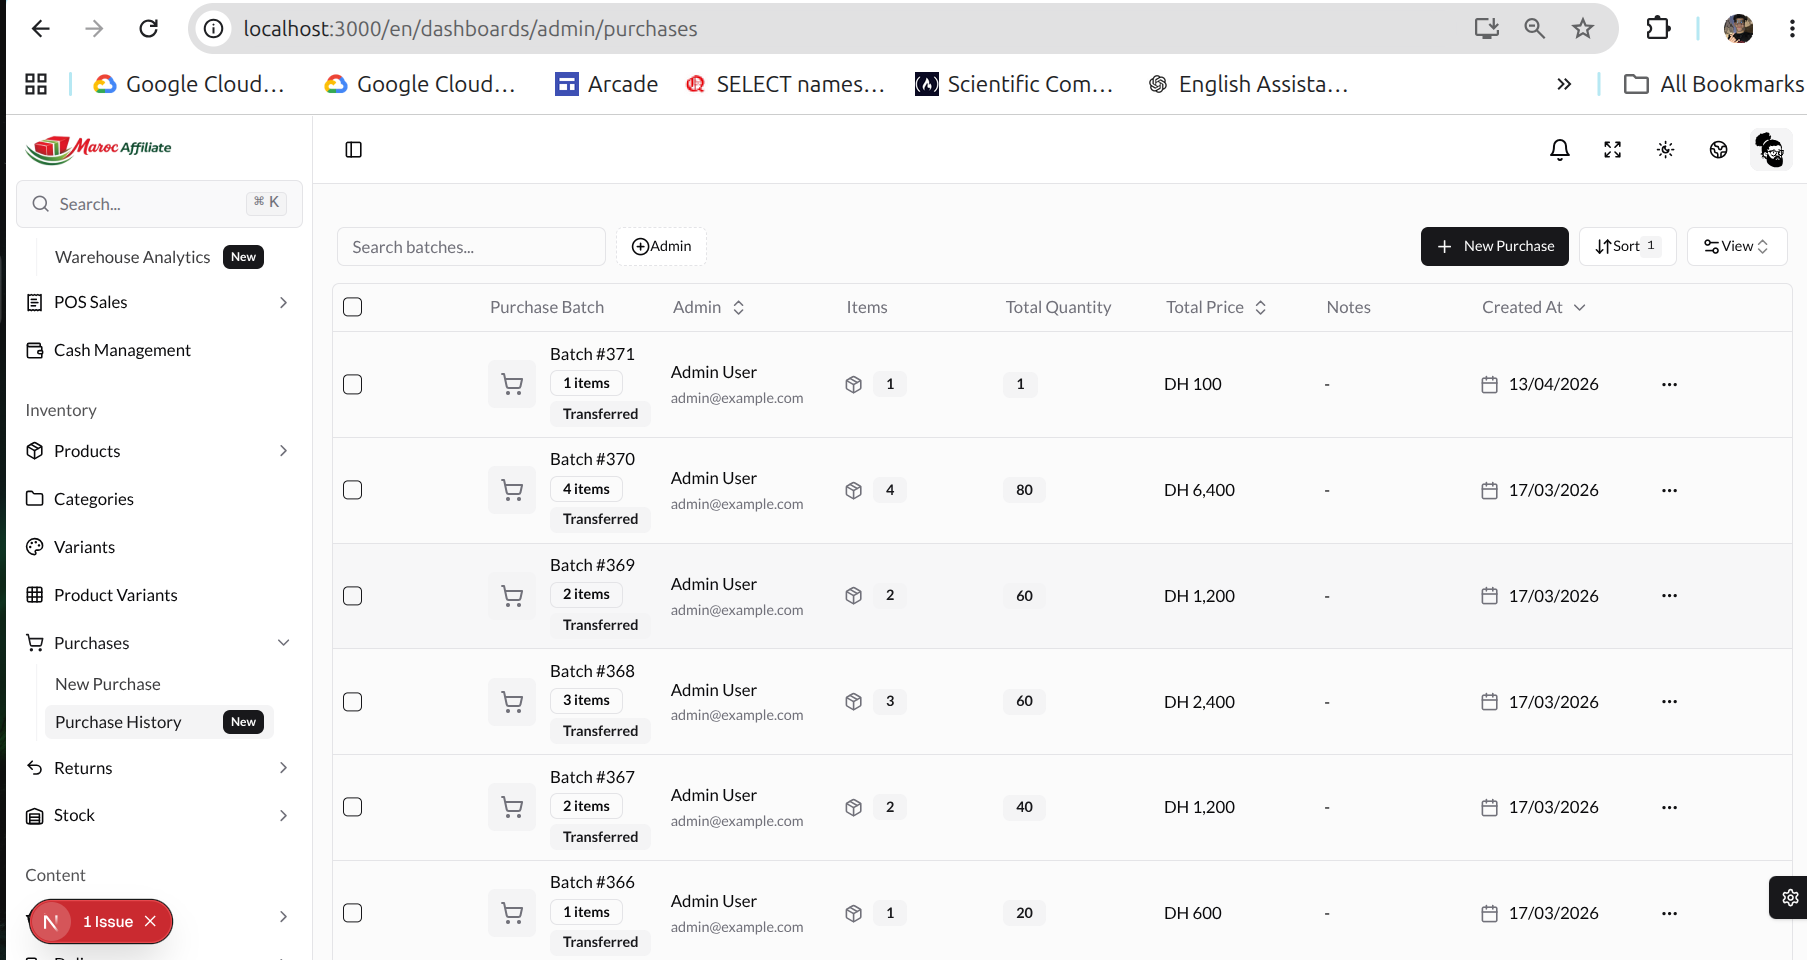
\includegraphics[width=\textwidth]{PFAimages/Screenshot from 2026-06-05 19-24-31.png}
\caption{Mode Scanner QR -- Champ auto-focus avec indicateur de queue et historique d'activité}
\end{figure}

\begin{figure}[H]
\centering
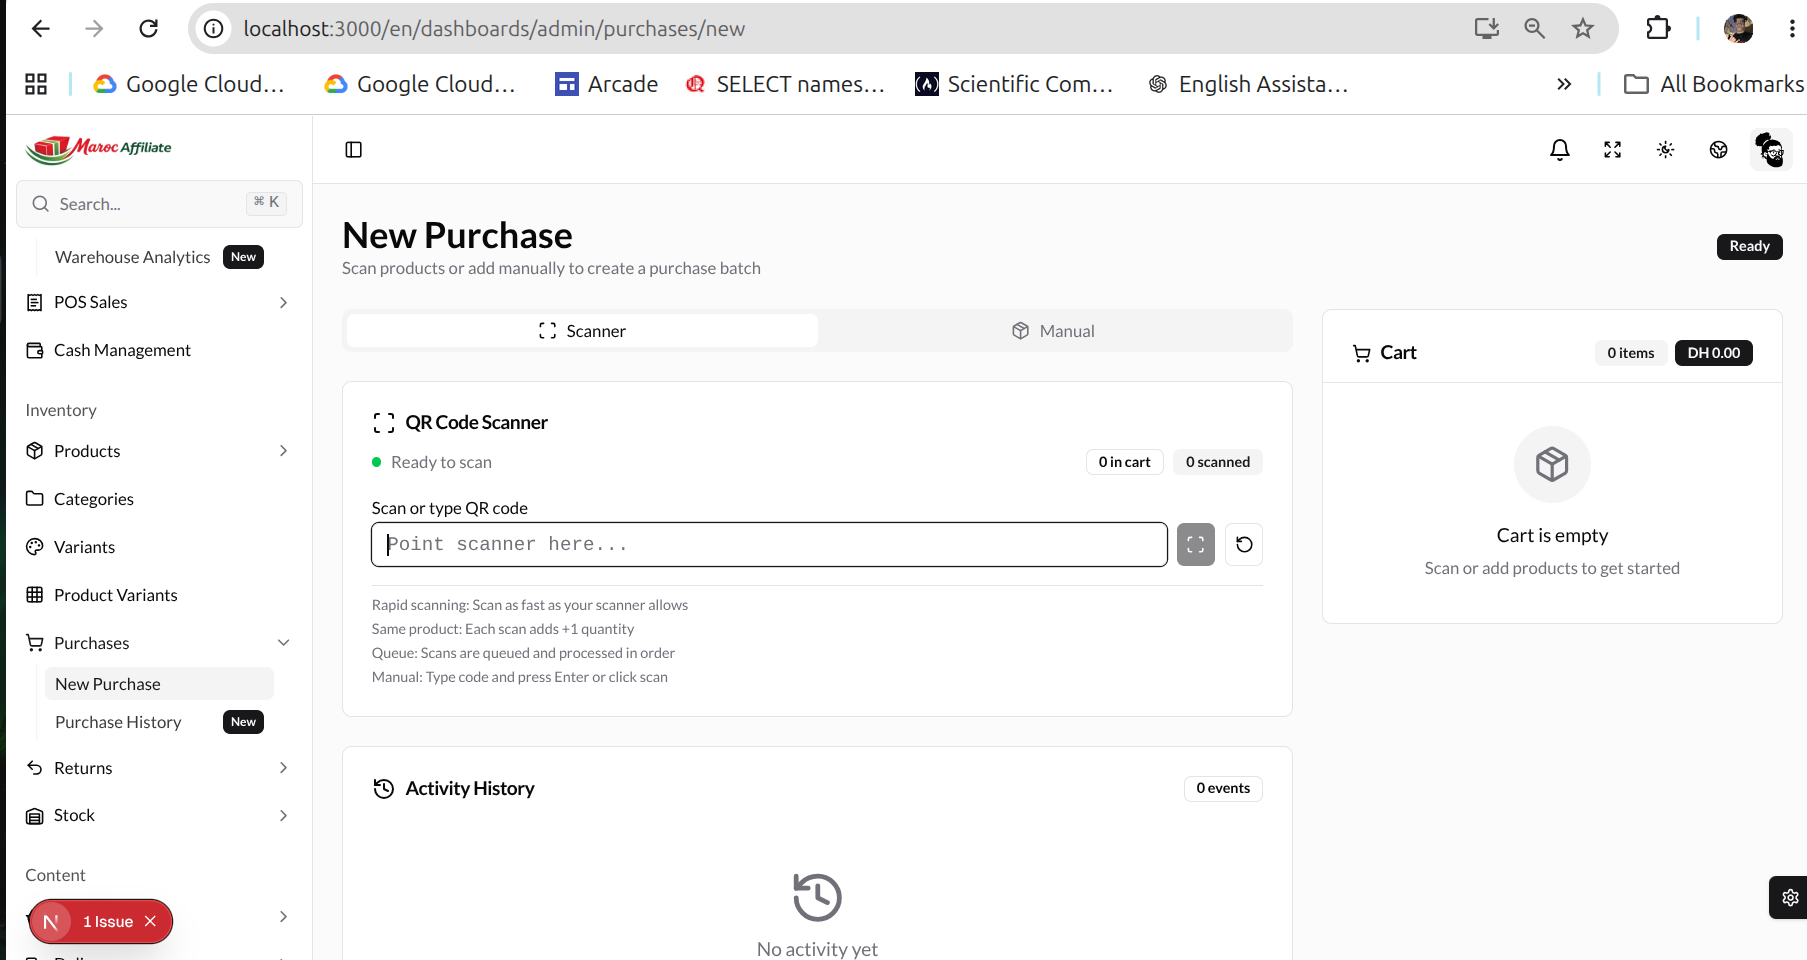
\includegraphics[width=\textwidth]{PFAimages/Screenshot from 2026-06-05 19-24-44.png}
\caption{Mode Scanner -- Panier d'achat rempli avec résumé (total articles, valeur MAD, fournisseurs)}
\end{figure}

On observe sur cette capture que le panier affiche en temps réel le nombre total d'articles (ici 12), la valeur cumulée en MAD, et le nombre de fournisseurs distincts concernés. Chaque ligne indique la méthode d'ajout (badge « Scanner ») et permet un ajustement rapide de la quantité. Ce résumé compact permet à l'opérateur de valider visuellement le contenu avant de lancer le traitement transactionnel.

\subsubsection{Mode Manuel}

Le mode manuel offre une interface de recherche avec filtres combinables (catégorie, fournisseur, statut). Le clic sur un produit ouvre un modal de sélection de variantes permettant de définir la quantité pour chaque combinaison couleur/taille individuellement.

\begin{figure}[H]
\centering
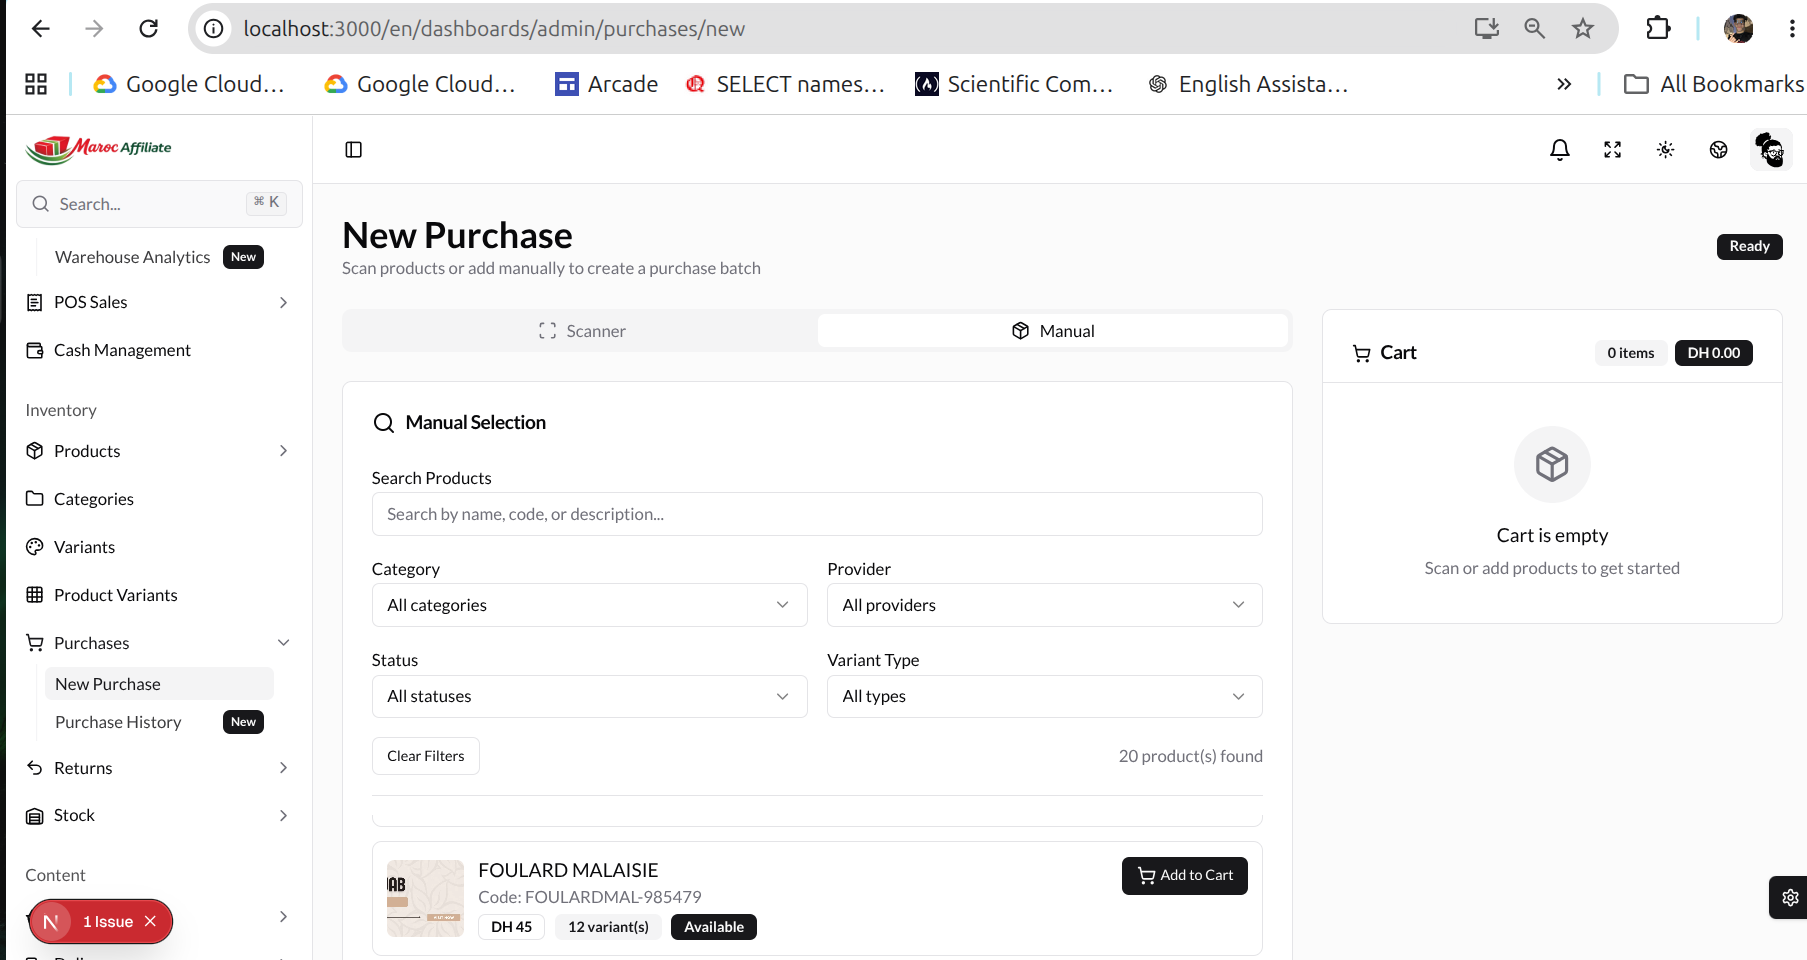
\includegraphics[width=\textwidth]{PFAimages/Screenshot from 2026-06-05 19-25-08.png}
\caption{Mode Manuel -- Grille de produits avec filtres par catégorie et fournisseur}
\end{figure}

\begin{figure}[H]
\centering
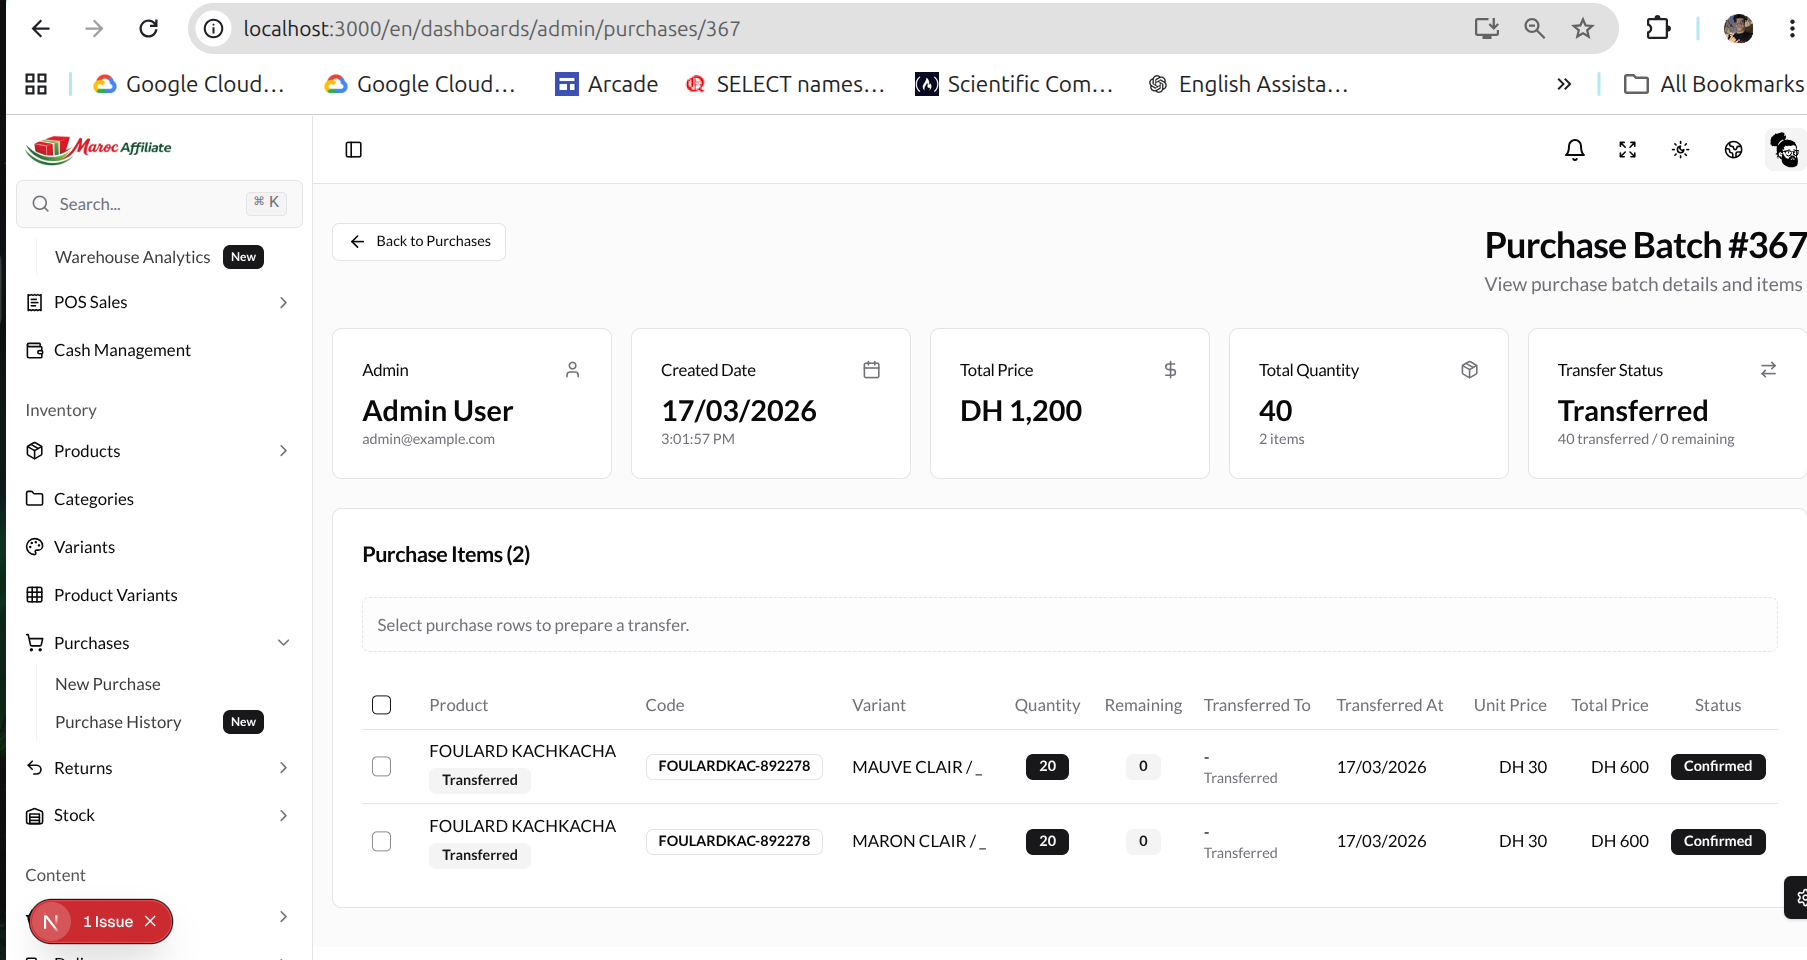
\includegraphics[width=\textwidth]{PFAimages/Screenshot from 2026-06-05 19-27-18.png}
\caption{Modal de sélection -- Quantité par variante avec fonction « Appliquer à toutes »}
\end{figure}

\subsubsection{Liste et détail des lots}

La page de liste affiche tous les lots d'achat avec filtres par administrateur et plage de dates. La page de détail permet la sélection multi-lignes avec quantités ajustables pour le transfert partiel vers les entrepôts opérationnels.

\begin{figure}[H]
\centering
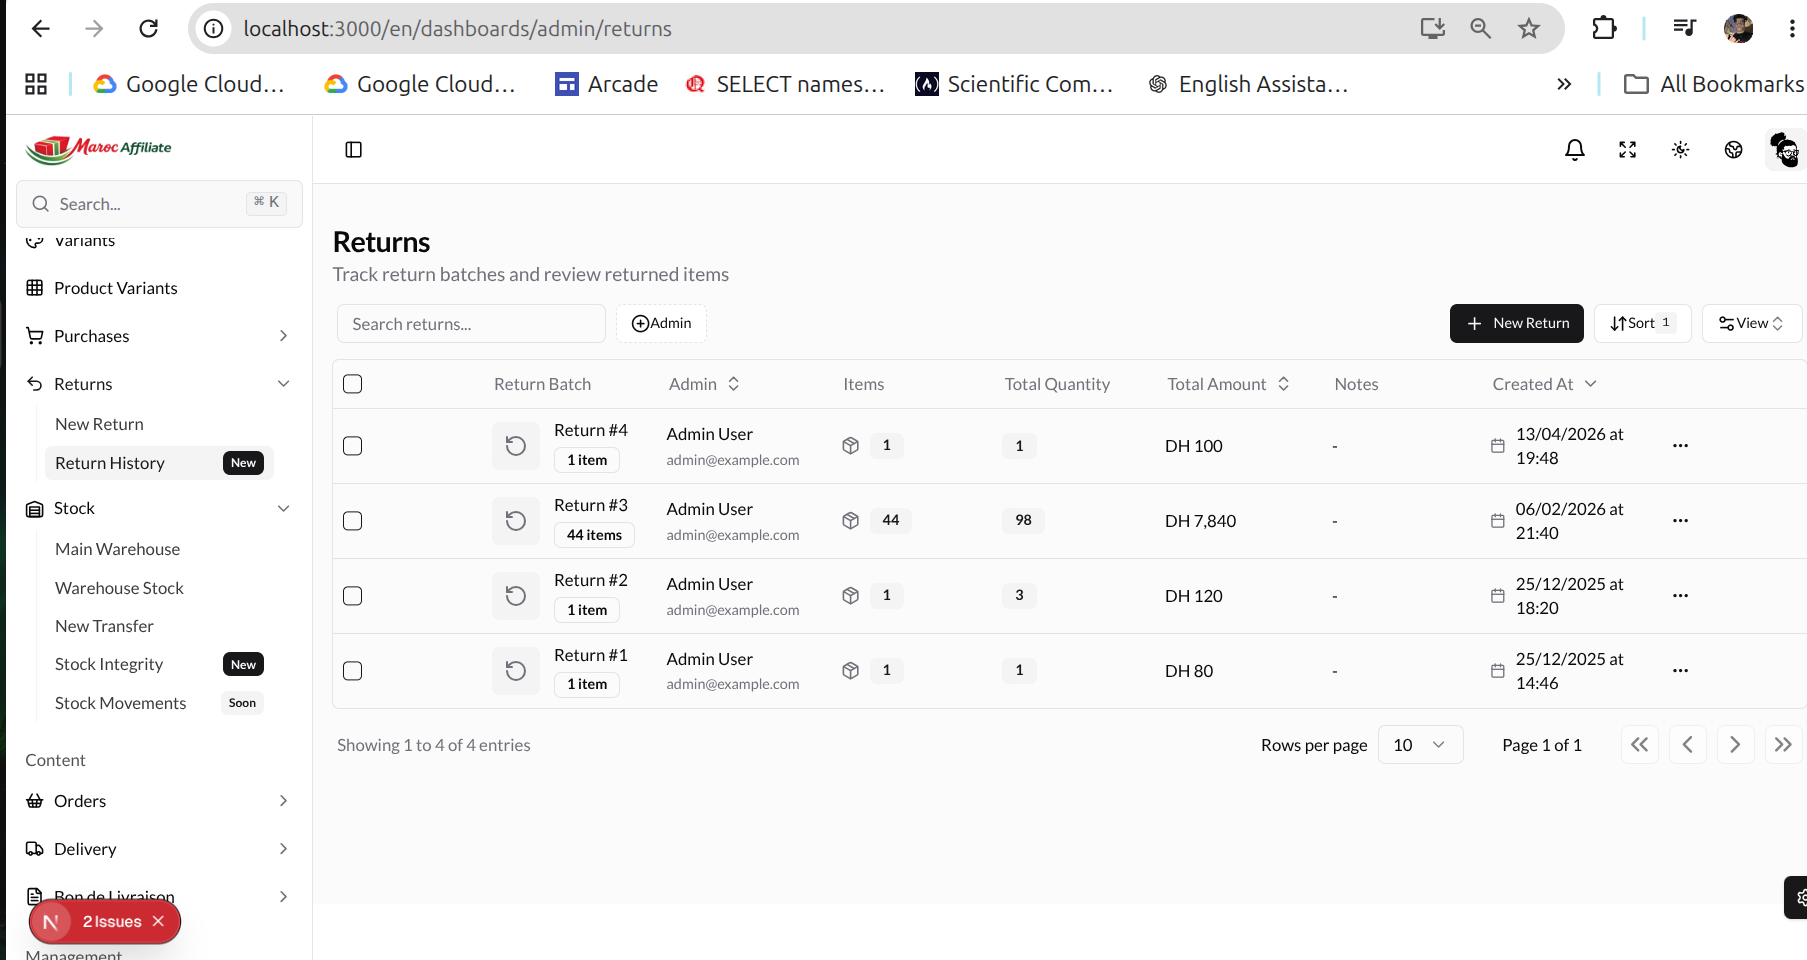
\includegraphics[width=\textwidth]{PFAimages/Screenshot from 2026-06-05 19-34-28.png}
\caption{Liste des lots -- DataTable avec filtres par admin, recherche et tri multi-colonnes}
\end{figure}

\begin{figure}[H]
\centering
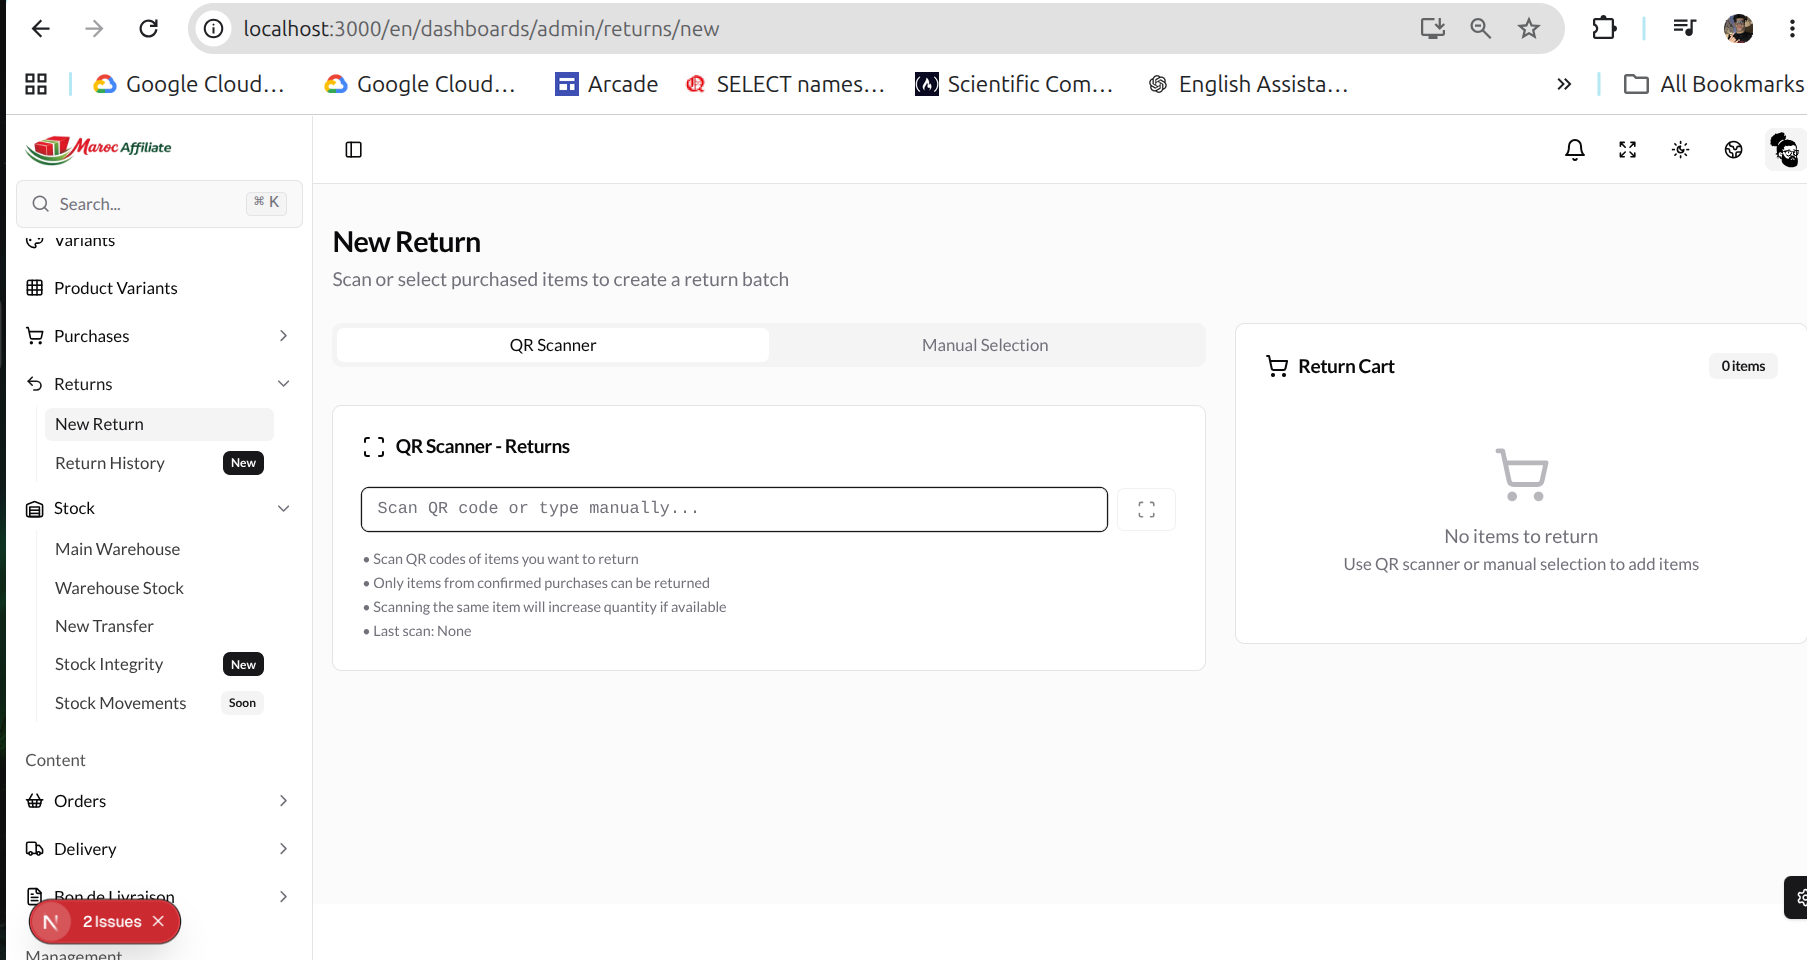
\includegraphics[width=\textwidth]{PFAimages/Screenshot from 2026-06-05 19-34-35.png}
\caption{Détail d'un lot -- Sélection multi-lignes avec badges de statut de transfert}
\end{figure}

\subsubsection{Transfert vers entrepôt}

Le dialog de transfert affiche le résumé des lignes sélectionnées et permet de choisir l'entrepôt de destination parmi les entrepôts actifs non-système.

\begin{figure}[H]
\centering
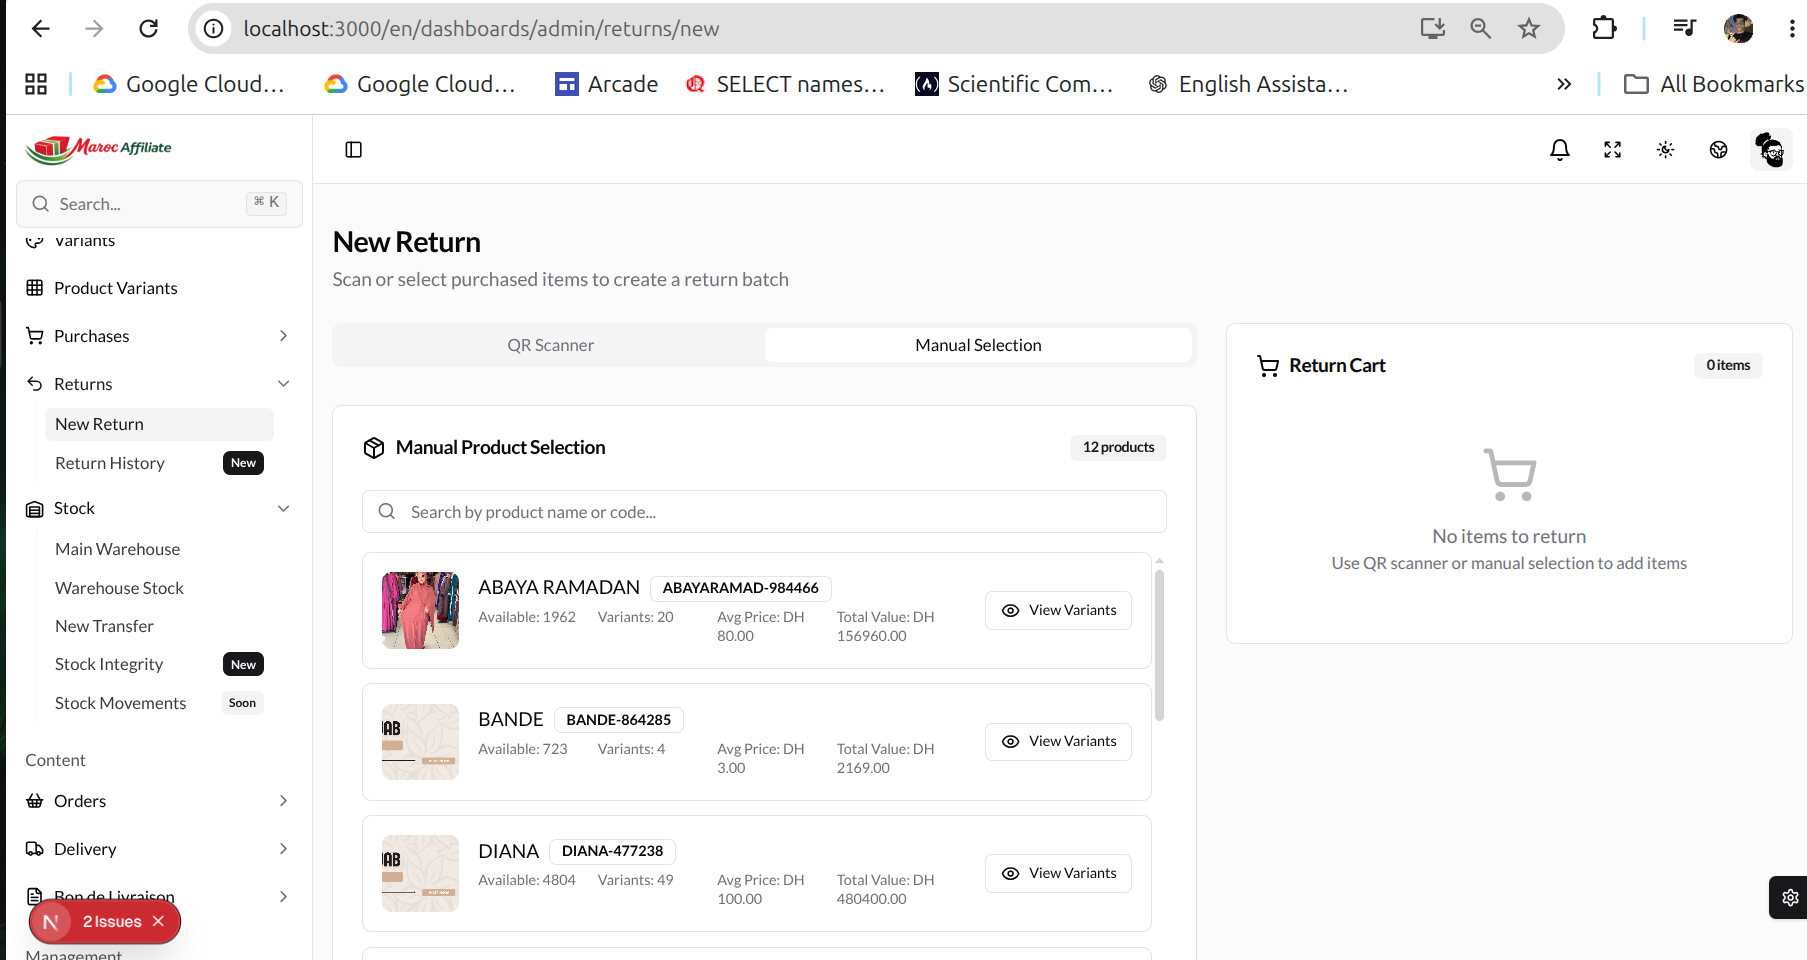
\includegraphics[width=\textwidth]{PFAimages/Screenshot from 2026-06-05 19-34-47.png}
\caption{Dialog de transfert -- Choix de l'entrepôt destination avec résumé des quantités}
\end{figure}

\subsection{Historique de développement}

Le développement a suivi une évolution architecturale en 6 phases, chaque transition étant motivée par un problème concret rencontré en production :

\begin{enumerate}
  \item \textbf{Phase 1 -- Scanner QR synchrone} : Première implémentation avec appel serveur bloquant à chaque scan. \textit{Problème :} quand l'opérateur scannait plus vite que la réponse serveur (environ 200\,ms), les scans étaient perdus car le champ input était bloqué.

  \item \textbf{Phase 2 -- Mode manuel ajouté} : Certains produits n'avaient pas encore d'étiquettes QR, nécessitant un mode de saisie alternatif avec recherche et filtres.

  \item \textbf{Phase 3 -- Refactoring basé sur une file d'attente} : Pour résoudre la perte de scans rapides, migration vers une file d'attente côté client. Le champ input reste libre et les scans sont traités séquentiellement. Choix préféré au debounce (fusion de scans distincts) et au mutex (blocage de l'input).

  \item \textbf{Phase 4 -- Internationalisation} : Support des opérateurs arabophones via les dictionnaires fr/en/ar avec RTL.

  \item \textbf{Phase 5 -- Transfert vers entrepôts} : Le stock entrant dans le Main Warehouse devait être distribué. Réutilisation du pipeline \code{executeTransfer} via une couche d'adaptation.

  \item \textbf{Phase 6 -- Transfert partiel} : Besoin de transférer une partie d'un lot (ex. : 50 sur 100 unités vers l'entrepôt A, le reste vers B). Ajout du champ \code{remainingQuantity} et des contrôles de quantité par ligne.
\end{enumerate}


% =============================================================================
\chapter[Difficultés, Bilan et Perspectives]{Difficultés Rencontrées, Bilan et Perspectives}

\section{Difficultés rencontrées et solutions apportées}

\subsection{Défis techniques transversaux}

\subsection{Performance des requêtes analytiques}

\textbf{Problème :} La vue exécutive du dashboard nécessitait 11 requêtes SQL complexes touchant les tables Order, DeliveryOrder, Customer, User, Product et Warehouse. L'exécution séquentielle engendrait des temps de chargement inacceptables (> 5s).

\textbf{Solution :}
\begin{enumerate}
  \item Parallélisation via \code{Promise.all()} -- réduction du temps d'environ 11× à 1× la requête la plus lente
  \item Cache agressif (TTL 300s) avec invalidation on-demand via \code{revalidateTag}
  \item Utilisation de \code{COUNT(*) FILTER (WHERE ...)} au lieu de multiples requêtes séparées
  \item Agrégations en une seule passe SQL avec CTEs
\end{enumerate}

\textbf{Résultat :} Temps de chargement < 1s en cache hit, < 3s en cache miss.

\subsection{Duplication de code entre modules}

\textbf{Problème :} Les 7 sous-pages analytics contenaient chacune une copie identique des helpers de dates et de validation, créant un risque de divergence.

\textbf{Solution :} Extraction dans un module utilitaire partagé \code{analytics/\_lib/utils.ts} importé par toutes les sous-pages. Un seul point de modification pour toute évolution.

\subsection{Staleness du cache après mutations}

\textbf{Problème :} Avec un TTL de 300s, un administrateur confirmant une commande ne voyait pas le changement reflété dans le dashboard pendant potentiellement 5 minutes.

\textbf{Solution :} Ajout de \code{revalidateTag("executive-summary")} dans les 12 server actions de mutation identifiées. La fraîcheur est devenue immédiate après toute opération.

\section{Défis du système de recommandation}

\subsection{Démarrage à froid pour les nouveaux vendeurs}

\textbf{Problème :} Un vendeur nouvellement inscrit n'a aucun historique de commandes, rendant la personnalisation impossible avec un algorithme basé uniquement sur l'historique.

\textbf{Solution :} Adaptation dynamique des poids~\ref{itm:ricci} -- pour un nouveau vendeur, le poids de la popularité (52,5\%) et de la nouveauté (37,5\%) est maximisé, tandis que l'historique et la récence sont à 0\%. À mesure que le vendeur accumule des commandes, les poids convergent vers la distribution standard.

\subsection{Problème N+1 dans le calcul des scores}

\textbf{Problème :} La première version calculait le score de chaque produit individuellement, générant des centaines de requêtes SQL par calcul de recommandation.

\textbf{Solution :} Refactoring vers des requêtes batch avec \code{GROUP BY} et \code{JOIN}.

\textbf{Résultats avant/après :}
\begin{itemize}
  \item Avant : environ 150 requêtes SQL par calcul (1 par produit candidat), temps total 2--4 secondes
  \item Après : 8 requêtes fixes par calcul (indépendant du nombre de produits), temps total 150--300ms
  \item Amélioration : \textbf{10--15× plus rapide}, passage de O(n) à O(1) en nombre de requêtes
\end{itemize}

\subsection{Dégradation gracieuse}

\textbf{Problème :} Une panne Redis ou un pic de charge sur PostgreSQL ne devait pas rendre le service totalement indisponible.

\textbf{Solution :} Stratégie multi-couches avec fallback : Redis → snapshot frais → snapshot périmé → popularité globale. Chaque niveau a un fallback garanti.

\section{Défis du module d'enrichissement de stock}

\subsection{Race conditions lors du scan rapide}

\textbf{Problème :} Un opérateur scannant rapidement plusieurs codes-barres en succession provoquait des appels serveur concurrents, avec risque de doublons ou de données incohérentes.

\textbf{Alternatives considérées :}
\begin{itemize}
  \item \textbf{Debounce (rejeté)} : Fusionnerait des scans distincts si l'intervalle est < seuil. Inadapté car chaque scan est un article unique.
  \item \textbf{Mutex / verrou (rejeté)} : Bloquerait le champ input pendant le traitement, causant la perte des scans effectués pendant l'attente.
  \item \textbf{Queue côté client (retenu)} : Le champ input reste toujours libre, chaque scan est empilé puis traité séquentiellement. Aucune perte.
\end{itemize}

\textbf{Résultats avant/après :}
\begin{itemize}
  \item Avant : 15--20\% de scans perdus lors de sessions rapides (> 1 scan/seconde)
  \item Après : 0\% de pertes, support confirmé jusqu'à 3 scans/seconde sans dégradation
\end{itemize}

\subsection{Atomicité des transactions d'achat}

\textbf{Problème :} La création d'un lot d'achat implique plusieurs opérations (Purchase + StockMovement + WarehouseStock + BarcodeScans). Une interruption au milieu pouvait laisser les données dans un état incohérent.

\textbf{Solution :} Transaction Prisma unique avec timeout de 60 secondes. Soit toutes les opérations réussissent, soit aucune n'est persistée.

\subsection{Transferts partiels}

\textbf{Problème :} Un lot d'achat de 100 unités devait pouvoir être transféré par portions vers différents entrepôts, avec suivi de la quantité restante.

\textbf{Solution :} Champ \code{remainingQuantity} sur le modèle Purchase, décrémenté à chaque transfert. Fonctions utilitaires dans \code{purchase-transfer.ts} pour calculer l'état (pending, partially transferred, fully transferred).

\section{Défis organisationnels}

\subsection{Cohérence multi-langue}

\textbf{Problème :} Maintenir la cohérence des traductions sur 3 langues (incluant RTL pour l'arabe) sur des modules complexes avec des dizaines de clés.

\textbf{Solution :} Structure hiérarchique des dictionnaires avec nommage explicite. Revue systématique des 3 fichiers lors de chaque ajout de clé.

\subsection{Intégration avec le système existant}

\textbf{Problème :} Le module d'enrichissement devait s'intégrer avec le pipeline de transfert inter-entrepôts existant (\code{StockTransfer} avec son lifecycle complet PENDING → APPROVED → IN\_TRANSIT → COMPLETED) sans le modifier ni introduire de régression.

\textbf{Solution :} Création d'une couche d'adaptation dédiée dans \code{src/lib/purchase-transfer.ts} qui transforme les données du domaine Purchase au format attendu par \code{executeTransfer}. Cette approche respecte le principe Open/Closed : le pipeline existant reste fermé à la modification mais ouvert à l'extension via un adaptateur.

\textbf{Résultat :} Zéro modification du code de transfert existant (1200+ lignes), intégration réalisée en 2 jours au lieu des 2 semaines estimées pour un pipeline dédié. Les transferts issus d'achats bénéficient automatiquement de toutes les fonctionnalités du pipeline standard (réservation de stock, génération de PDF, gestion des écarts à la réception).

\section{Bilan du module d'enrichissement}

Le module d'enrichissement de stock est en production et couvre l'intégralité du cycle d'approvisionnement. Il a permis de réduire le temps de réception de stock de 2 heures (saisie manuelle sur tableur) à 15 minutes (scan QR), avec zéro erreur de comptage grâce aux transactions atomiques et à la traçabilité complète.

\begin{itemize}
  \item \textbf{Système complet et opérationnel} couvrant l'intégralité du cycle d'approvisionnement
  \item \textbf{Deux modes d'entrée} adaptés aux différents contextes opérationnels (scan rapide et sélection manuelle)
  \item \textbf{Intégration transactionnelle} avec traçabilité complète (audit trail)
  \item \textbf{Pipeline de transfert} réutilisant l'infrastructure existante sans modification
\end{itemize}

% =============================================================================
% CONCLUSION GÉNÉRALE
% =============================================================================
\chapter*{Conclusion Générale}
\addcontentsline{toc}{chapter}{Conclusion Générale}
\markboth{Conclusion Générale}{Conclusion Générale}

Ce stage de fin d'année au sein de Maroc Affiliate Network m'a permis de concevoir et développer trois modules stratégiques pour une plateforme e-commerce d'affiliation en production.

\textbf{Le module Analytics Dashboard} fournit aux administrateurs une vision opérationnelle complète à travers 8 tableaux de bord et 50+ indicateurs, avec un système de cache intelligent garantissant des temps de réponse inférieurs à la seconde.

\textbf{Le système de recommandation TrackA} est un microservice autonome déployé sur Railway qui personnalise l'expérience des vendeurs via un algorithme à 5 signaux adaptatif. Avec un temps de réponse < 5ms en régime nominal et une architecture résiliente à 5 niveaux de fallback, il répond aux exigences de performance d'une plateforme en croissance.

\textbf{Le module d'enrichissement de stock} optimise le processus d'approvisionnement grâce à un double mode d'entrée (scan QR rapide et sélection manuelle), des transactions atomiques, et une intégration transparente avec le pipeline de transfert inter-entrepôts existant.

\vspace{0.5cm}

\begin{table}[H]
\centering
\rowcolors{2}{rowgray}{white}
\begin{tabularx}{\textwidth}{lXl}
\toprule
\rowcolor{headerblue!20}
\textbf{Objectif initial} & \textbf{Réalisation} & \textbf{Statut} \\
\midrule
Système d'analytics avancé & 8 dashboards, 50+ KPIs, cache intelligent & \checkmark Atteint \\
Moteur de recommandation & Microservice autonome, 5 signaux, < 5ms & \checkmark Atteint \\
Module d'enrichissement stock & Dual-mode (QR + manuel), transactions atomiques & \checkmark Atteint \\
\bottomrule
\end{tabularx}
\caption{Vérification de l'atteinte des objectifs}
\end{table}

\textbf{Perspectives d'évolution :}
\begin{itemize}
  \item Intégration d'un modèle ML supervisé pour les recommandations (A/B testing)
  \item Vues matérialisées PostgreSQL pour les agrégations analytiques lourdes
  \item Import CSV/Excel pour les achats en gros volume
  \item Application mobile dédiée pour le scan d'inventaire
  \item Dashboard en temps réel avec WebSockets pour les métriques critiques
\end{itemize}

Ce stage m'a offert l'opportunité de travailler sur un projet d'envergure en production. La combinaison de Next.js 15~\ref{itm:nextjs} pour le monolithe et de FastAPI~\ref{itm:fastapi} pour les microservices s'est révélée efficace, offrant la productivité d'un framework full-stack moderne et la flexibilité de services spécialisés.

Ce qui m'a le plus marqué est le passage de la théorie à la pratique pour l'algorithme de recommandation : la conception mathématique était la partie facile, tandis que les vrais défis étaient opérationnels (cold-start, invalidation de cache, dégradation gracieuse). Cette expérience a profondément changé ma vision du développement logiciel et constitue un socle solide pour la suite de ma carrière d'ingénieur.

Sur le plan personnel, ce stage m'a permis de développer des compétences transversales essentielles : la capacité à concevoir des architectures distribuées résistantes aux pannes, la maîtrise des compromis entre complexité technique et valeur métier, et l'habitude de valider chaque hypothèse par des mesures en production. La collaboration quotidienne avec l'encadrant entreprise m'a également appris l'importance du pragmatisme dans les décisions d'ingénierie : choisir la solution « suffisamment bonne » qui peut être livrée rapidement, plutôt que la solution théoriquement optimale qui ne verra jamais le jour.

% =============================================================================
% BIBLIOGRAPHIE
% =============================================================================
\chapter*{Bibliographie}
\addcontentsline{toc}{chapter}{Bibliographie}
\markboth{Bibliographie}{Bibliographie}

\begin{enumerate}[label={[\arabic*]}]
  \item \label{itm:nextjs} Vercel. \textit{Next.js 15 Documentation -- App Router}. \url{https://nextjs.org/docs}. Consulté en 2026.

  \item \label{itm:prisma} Prisma. \textit{Prisma ORM Documentation}. \url{https://www.prisma.io/docs}. Consulté en 2026.

  \item \label{itm:fastapi} Ramírez, S. \textit{FastAPI Documentation}. \url{https://fastapi.tiangolo.com}. Consulté en 2026.

  \item \label{itm:koren} \label{cite:koren2009} Koren, Y. (2009). \textit{Collaborative Filtering with Temporal Dynamics}. Proceedings of KDD 2009. -- Référence pour les approches de décroissance temporelle dans les systèmes de recommandation.

  \item \label{itm:ricci} Ricci, F., Rokach, L., Shapira, B. (2015). \textit{Recommender Systems Handbook}. Springer. -- Fondements théoriques des ensembles pondérés et du cold-start.

  \item \label{itm:nextauth} NextAuth.js. \textit{NextAuth v5 Documentation}. \url{https://authjs.dev}. Consulté en 2026.

  \item \label{itm:redis} Redis Ltd. \textit{Redis Documentation -- Caching Patterns}. \url{https://redis.io/docs}. Consulté en 2026.

  \item \label{itm:bullmq} Taskforce.sh. \textit{BullMQ Documentation}. \url{https://docs.bullmq.io}. Consulté en 2026.

  \item \label{itm:tailwind} Tailwind Labs. \textit{Tailwind CSS v4 Documentation}. \url{https://tailwindcss.com/docs}. Consulté en 2026.

  \item \label{itm:prometheus} Prometheus Authors. \textit{Prometheus Documentation}. \url{https://prometheus.io/docs}. Consulté en 2026.

  \item \label{itm:neon} Neon Inc. \textit{Neon Serverless PostgreSQL}. \url{https://neon.tech/docs}. Consulté en 2026.

  \item \label{itm:railway} Railway. \textit{Railway Deployment Platform}. \url{https://docs.railway.app}. Consulté en 2026.
\end{enumerate}

% =============================================================================
% FIN DU DOCUMENT
% =============================================================================
\end{document}
